% Latex main.tex file for Xiaochuan Tian's Master Thesis at the University of Memphis
% Advisor: Dr. Eunseo Choi
% Date: 2015,February ~ April
% Location: Center for Earthquake Research and Information
% Title: 3D Numerical Models for Along-axis Variations in Diking at Mid-Ocean Ridges
% The format and structure according to: Thesis requirements from the University of Memphis: 
% http://www.memphis.edu/gradschool/tdinfo_electronic.php#samplepages (referred as RQ(Requirements) in the code)
% <> is refered as a symbol for question or problem needed to be answered or solved
% Samples of recent submitted Thesis can be found from:
% https://umwa.memphis.edu/etd/

%%-----------------------------------------------------
%% Thesis Environments Setup
%%-----------------------------------------------------

\documentclass[12pt]{article}  % RQ 3.1

\usepackage{times}             % RQ 3.1 (this is not exactly times new roman but very similar)
\usepackage[top=1.0in, right=1.0in, bottom=1.0in, left=1.5in]{geometry} % RQ 3.2
% <> RQ 3.2 0.5inches for page numbers postistion haven't been added
\usepackage{setspace}
\doublespacing                 % RQ 3.4
\renewcommand{\contentsname}{\textit{\small{Table of Contents}}}  % Change from Contents to Table of Contents
\usepackage{hyperref}    % For hyperlinks to contents
%Ref: http://en.wikibooks.org/wiki/LaTeX/Hyperlinks
\hypersetup{
    %hidelinks             % If you don't like the color for links, uncomment this
    colorlinks=true,       % false: boxed links(no colors); true: colored links
    linkcolor=red,          % color of internal links (change box color with linkbordercolor)
    citecolor=green,        % color of links to bibliography
    filecolor=magenta,      % color of file links
    urlcolor=cyan           % color of external links
}
% The format is e.g. for figures: "Figure~\hyperref["label name"]{\ref{"label name"}}" left for what to link, right for what to show as  the link.
% In Mac OS Preview for viewing the pdf file, after clicking the link, simply try ("cmd"+"[") will help to go back.
% ref: http://apple.stackexchange.com/questions/90032/mac-os-preview-linked-pdf-and-going-back 

\usepackage{natbib}  %for \citep

\usepackage{graphics}
\usepackage{epsfig}

\usepackage{amsmath}
%\usepackage{float}  % for floating figures
\usepackage{floatrow} %for caption of figures on its side
\usepackage{gensymb} %for \degree
\usepackage{subcaption} %for figures side by side

\usepackage{diagbox} % for table cell with a diagonal line and 2 sub cells

%\setcounter{secnumdepth}{5} %for \paragragh
%%------------------------------------------------ 
% For trackchanges.sty  (For co-revision)
% Change the editor name as you like         
%%------------------------------------------------
\usepackage[inline]{trackchanges}
\addeditor{XT}
\addeditor{EC}
%%------------------------------------------------
% Try one of these commands:
%     \add[editor]{added text}
%     \remove[editor]{removed text}
%     \change[editor]{removed text}{added text}
%     \note[editor]{note text}
%     \annote[editor]{text to annotate}{note text}
%%------------------------------------------------   

%%-------------------------------------------------
% \includeonly files that have been made changes for 
%     faster processing during revision processes
%%-------------------------------------------------

% Uncomment the following line will process the whole file.

\includeonly{Title_Page, Copyright_Notice, Dedication, Acknowledgements, Abstract, Table_of_Contents, Introduction, Methods, Results, Discussion, Conclusions}

% Comment the previous line and type below the chapter you are frequently making changes.

%\includeonly{Results}

%%-----------------------------------------------------
%% Thesis Begin
%%-----------------------------------------------------

\begin{document}

%%--------------------------------------------------
% Preleminary Pages
%%--------------------------------------------------
\pagenumbering{roman}


\thispagestyle{empty}  % For hiding the page number at the title page

\newgeometry{top=2.0in, left=1.5in}

\begin{center}


\uppercase{3D Numerical Models for Along-axis Variations in Diking at Mid-Ocean Ridges}
\\
\vspace{10pt}
by
\vspace{10pt}
\\
Tian, Xiaochuan
\\
\begin{CJK}{UTF8}{gbsn}
田小川
\end{CJK}
\\
\vspace{100pt}

A Thesis
\\
%\vspace{2pt}
Submitted in Partial Fulfillment of the 
\\
%\vspace{2pt}
Requirements for the Degree of 
\\
%\vspace{2pt}
Master of Science
\\
\vspace{35pt}

Major: Earth Sciences
\\

\vspace{120pt}

The University of Memphis
\\

August, 2015

\end{center}

\restoregeometry

\begin{center}
  \vspace*{\fill}
Copyright \copyright \ 2015 Xiaochuan Tian
\\All rights reserved
  \vspace*{\fill}
\end{center}
 % optional
\begin{center}
\textbf{\textit{Dedication}}
\end{center}

I would like to dedicate this thesis to my mother, Xia Tian. I wouldn't have a chance to experience this wonderful world without her giving birth to me. She rears me up by herself with her great love, optimism and peseverence. Without her guidance and support, I will not become who I am.

I also want to dedicate this thesis toward my major thesis advisor: Dr. Eunseo Choi. His mentorship defines what a great advisor is like. Without his  guidance, neither this theis nor my fast personal-development during these two years is possible. He has kindled a flame that illuminates the way for my future career as a geodynamic modeler.   

 % optional
\begin{center}
\textbf{\textit{Acknowledgements}}
\end{center}

To Eunseo,
\\
To Committee members,
\\
To CERI, 
 % optional
%\include{Preface} % optional
\begin{center}
\textbf{\textit{Abstract}}
\end{center}

\vspace{0.5cm}

\begin{singlespace*}
Tian, Xiaochuan. M.S. The University of Memphis. May 2015 Master of Science. 3D Numerical Models for Along-axis Variations in Diking at Mid-Ocean Ridges. Major Professor: Eunseo Choi.
\end{singlespace*}

\vspace{0.5cm}

Bathymetry of ocean floors reveals a great variety of morphologies at Mid-ocean Ridges (MORs). Previous studies showed that the morphologies at slow spreading MORs are mainly controlled by the ratio between rates of magma supply and plate extension. 2D models for the across-ridge cross-sections have been successful in explaining many of the observed morphological features such as abyssal hills and oceanic core complexes. However, the magma supply varies along the ridge and the interaction between the tectonic plates and magmatism at MORs are inevitably 3D processes. We propose to investigate the consequences of the along-axis variability in diking in terms of faulting pattern and the associated structures. This work will include implementation of an algorithm of parameterizing repeated diking in a 3D parallel geodynamic modeling code.



\begin{center}
\tableofcontents
\addtocontents{toc}{{Chapter}}
\addtocontents{toc}{~\hfill{Page}\par}
\end{center}

%\begin{center}
        \listoftables
\end{center}

 % for 5 or more
%\begin{center}
        \listoffigures
\end{center}

 % for 5 or more
%\include{Key_to_Symbols_or_Abbreviations} % optional

%%--------------------------------------------------
% Text
%%--------------------------------------------------
\pagenumbering{arabic}

\pagebreak
\section{Introduction}
\label{ch:Intro}  % <>? why ch: befor Intro

\subsection{Review of Literature}

Geodynamic modeling as well as a variety of geological, geophysical observations and lab experiments have provided insight into the processes occurring at the mid-ocean ridges (MORs) \citep[e.g.,][]{Tucholke1994,Blackman2004,Behn2006,Behn2008,Ito2008,Baines2008,Escartin2008,Canales2008,Dick2008,Dannowski2010,Olive2010,Reston2011a,Reston2011b}. In particular, the advent of high-resolution multi-beam bathymetric data has made it possible to discover differences in axial topography between slow and fast spreading ridges and morphological transition from the center of a ridge segment to the tip of the ridge segment.

Variations in morphologies among different MORs are mainly controlled by four factors: magma supply, tectonic strain, hydrothermal circulation and spreading rate \citep{Fowler2004}.
%\add[XT]{Clarify the relationship between the four factors and try to cite the original work for each of them. (in Fowler2004, they didn't mention the ref for these four factors, page417 Chapter9.4.1)} 
Among them, the spreading rate shows the strongest correlation with the ridge morphology. Slow-to-intermediate spreading ridges (half spreading rate less than 4 cm/yr) produce median valleys that are typically 10$\sim$20 km wide and 1$\sim$2 km deep (e.g., Mid-Atlantic Ridges, Figure \ref{fig_Intro1_1}). Fast-spreading ridges (half spreading rate greater than 5 cm/yr) like the East Pacific Rise have axial highs that are 10$\sim$20 km wide, 0.3$\sim$0.5 km high (Figure~\hyperref[fig_Intro1_3]{\ref{fig_Intro1_3}}).
\begin{figure}[h]
\centering
\begin{subfigure}{.5\textwidth}
  \centering
  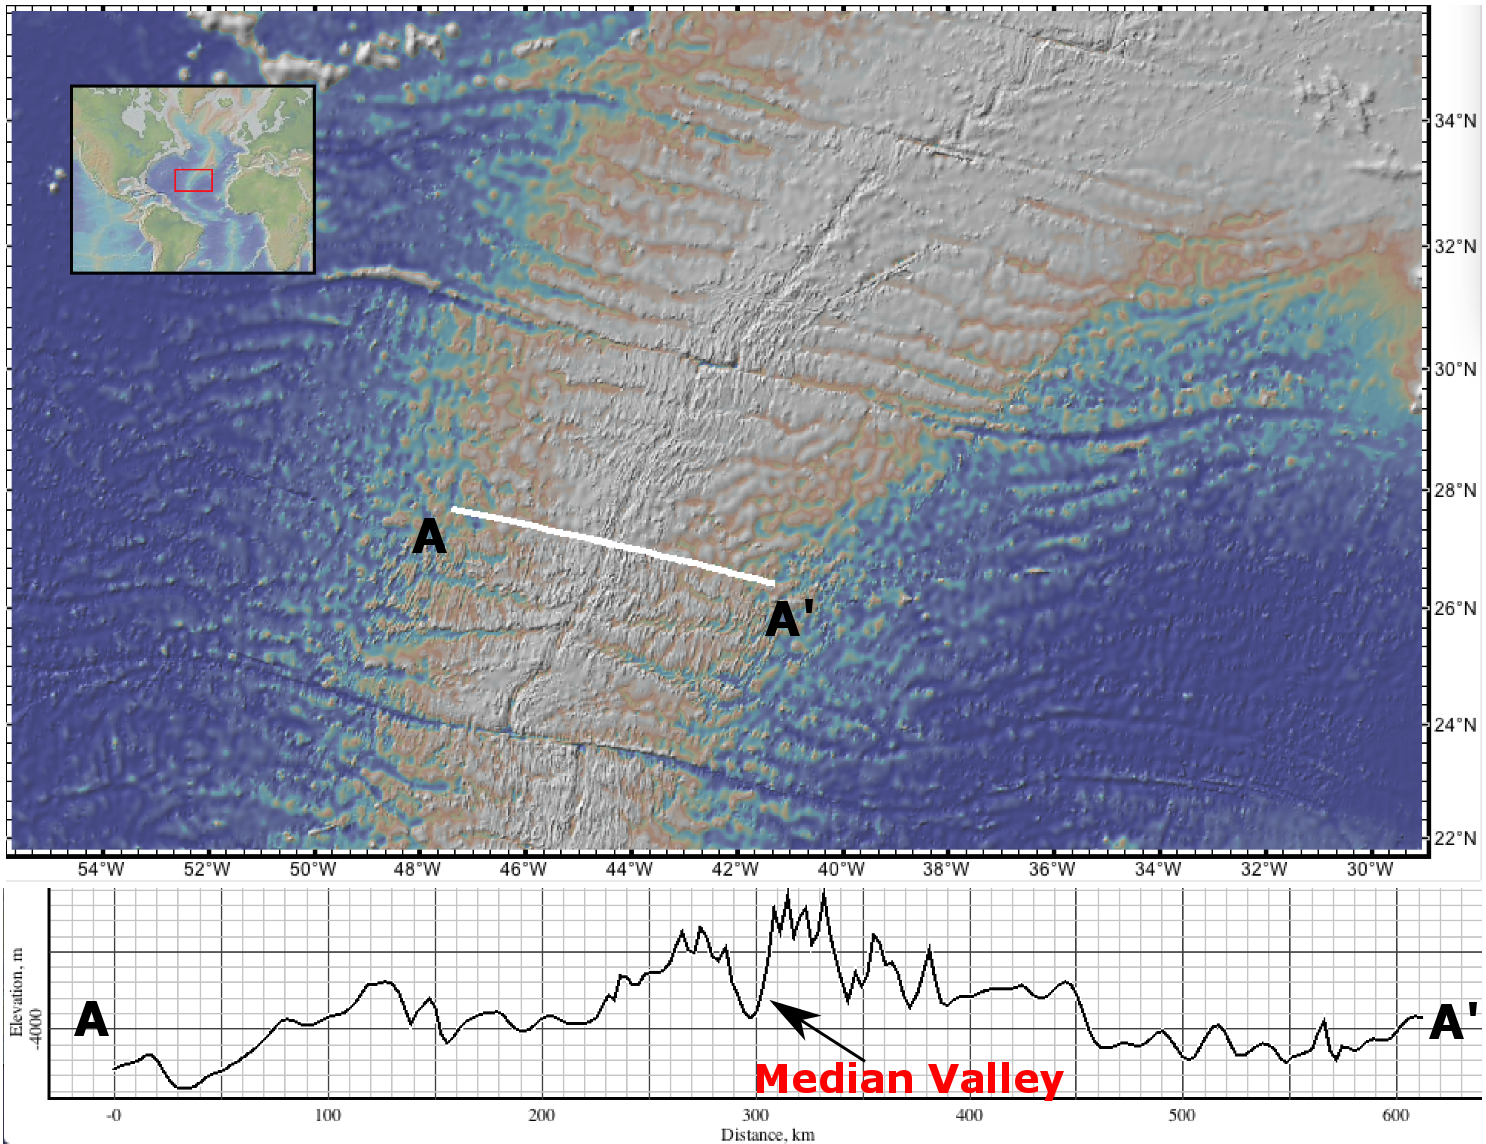
\includegraphics[width=.8\linewidth]{./Figures/fig_Intro1_1.png}
  \caption{\small{Slow spreading Mid-Atlantic Ridge}}
  \label{fig_Intro1_1}
\end{subfigure}%
\begin{subfigure}{.5\textwidth}
  \centering
  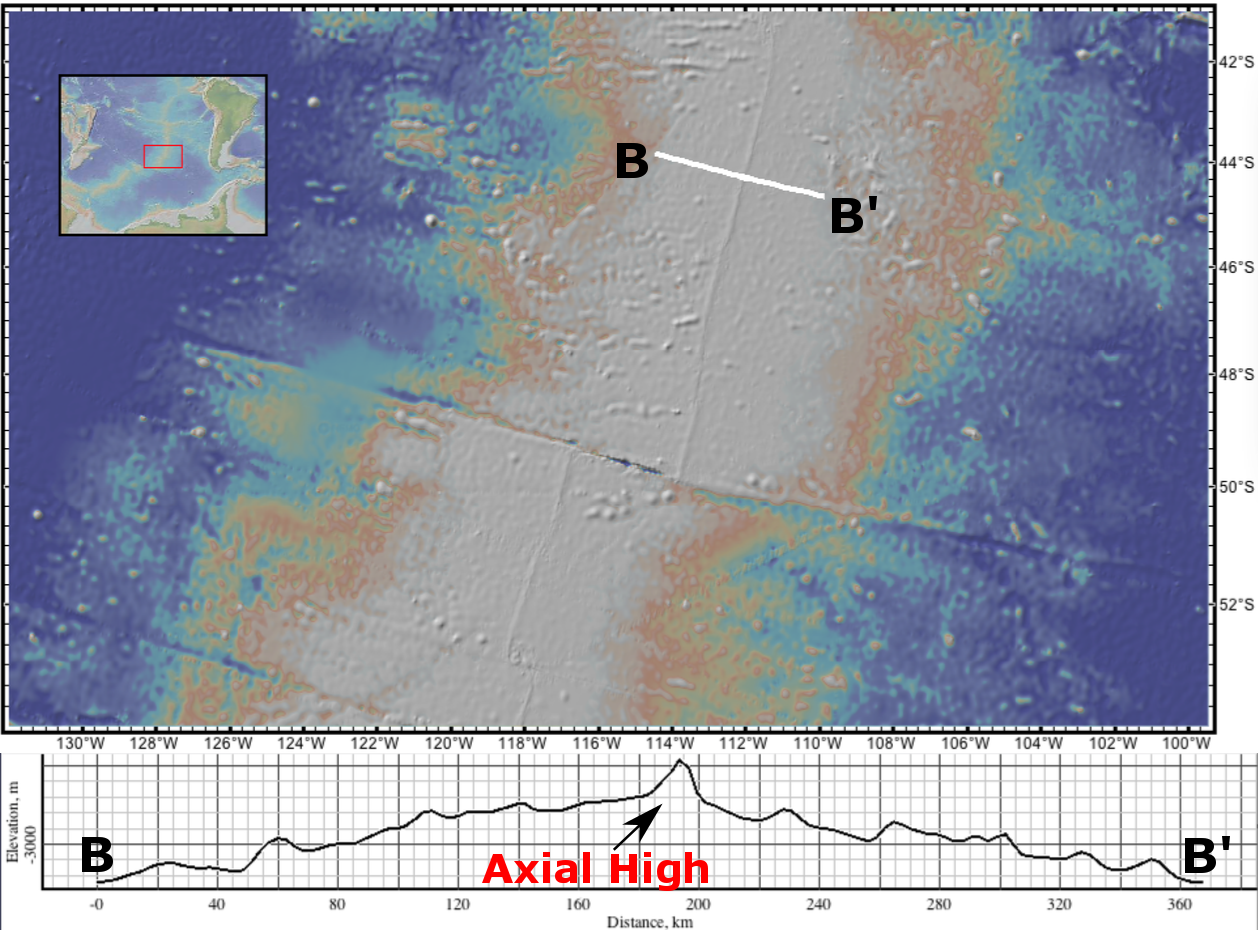
\includegraphics[width=.8\linewidth]{./Figures/fig_Intro1_3.png}
  \caption{\small{Fast spreading East Pacific Rise}}
  \label{fig_Intro1_3}
\end{subfigure}
\caption{Profiles of bathymetry across MORs.}
\end{figure}

Slow spreading ridges exhibit along-axis variations in off-axis morphology, the width and depth of median valleys and crustal thickness.  Figure~\ref{fig_Intro2_1} shows that the topographic profile near the center of the ridge segment (A-A$^{\prime}$) is rather symmetrical and has a shorter wavelength with a median valley $\sim$12 km wide and $\sim$1 km deep. In constrast, the near-tip profile (B-B$^{\prime}$) is asymmetrical and has a much longer wavelength with a median valley wider than 30 km and shows a greater relief ($\sim$3 km). Gravity data of different ridge segments along MAR (28$\sim$31 $\degree$N and 33$\sim$37 $\degree$N) suggests that the maximum along-axis variation in crustal thickness $\Delta H_{c}$ of a single segment increases with the segment length L \citep{Chen1999} and the relationship is $\Delta H_{c}$(L) = 0.0206L (Figure~\ref{fig_Intro3_1}).

\begin{figure}[H]
 \centering
  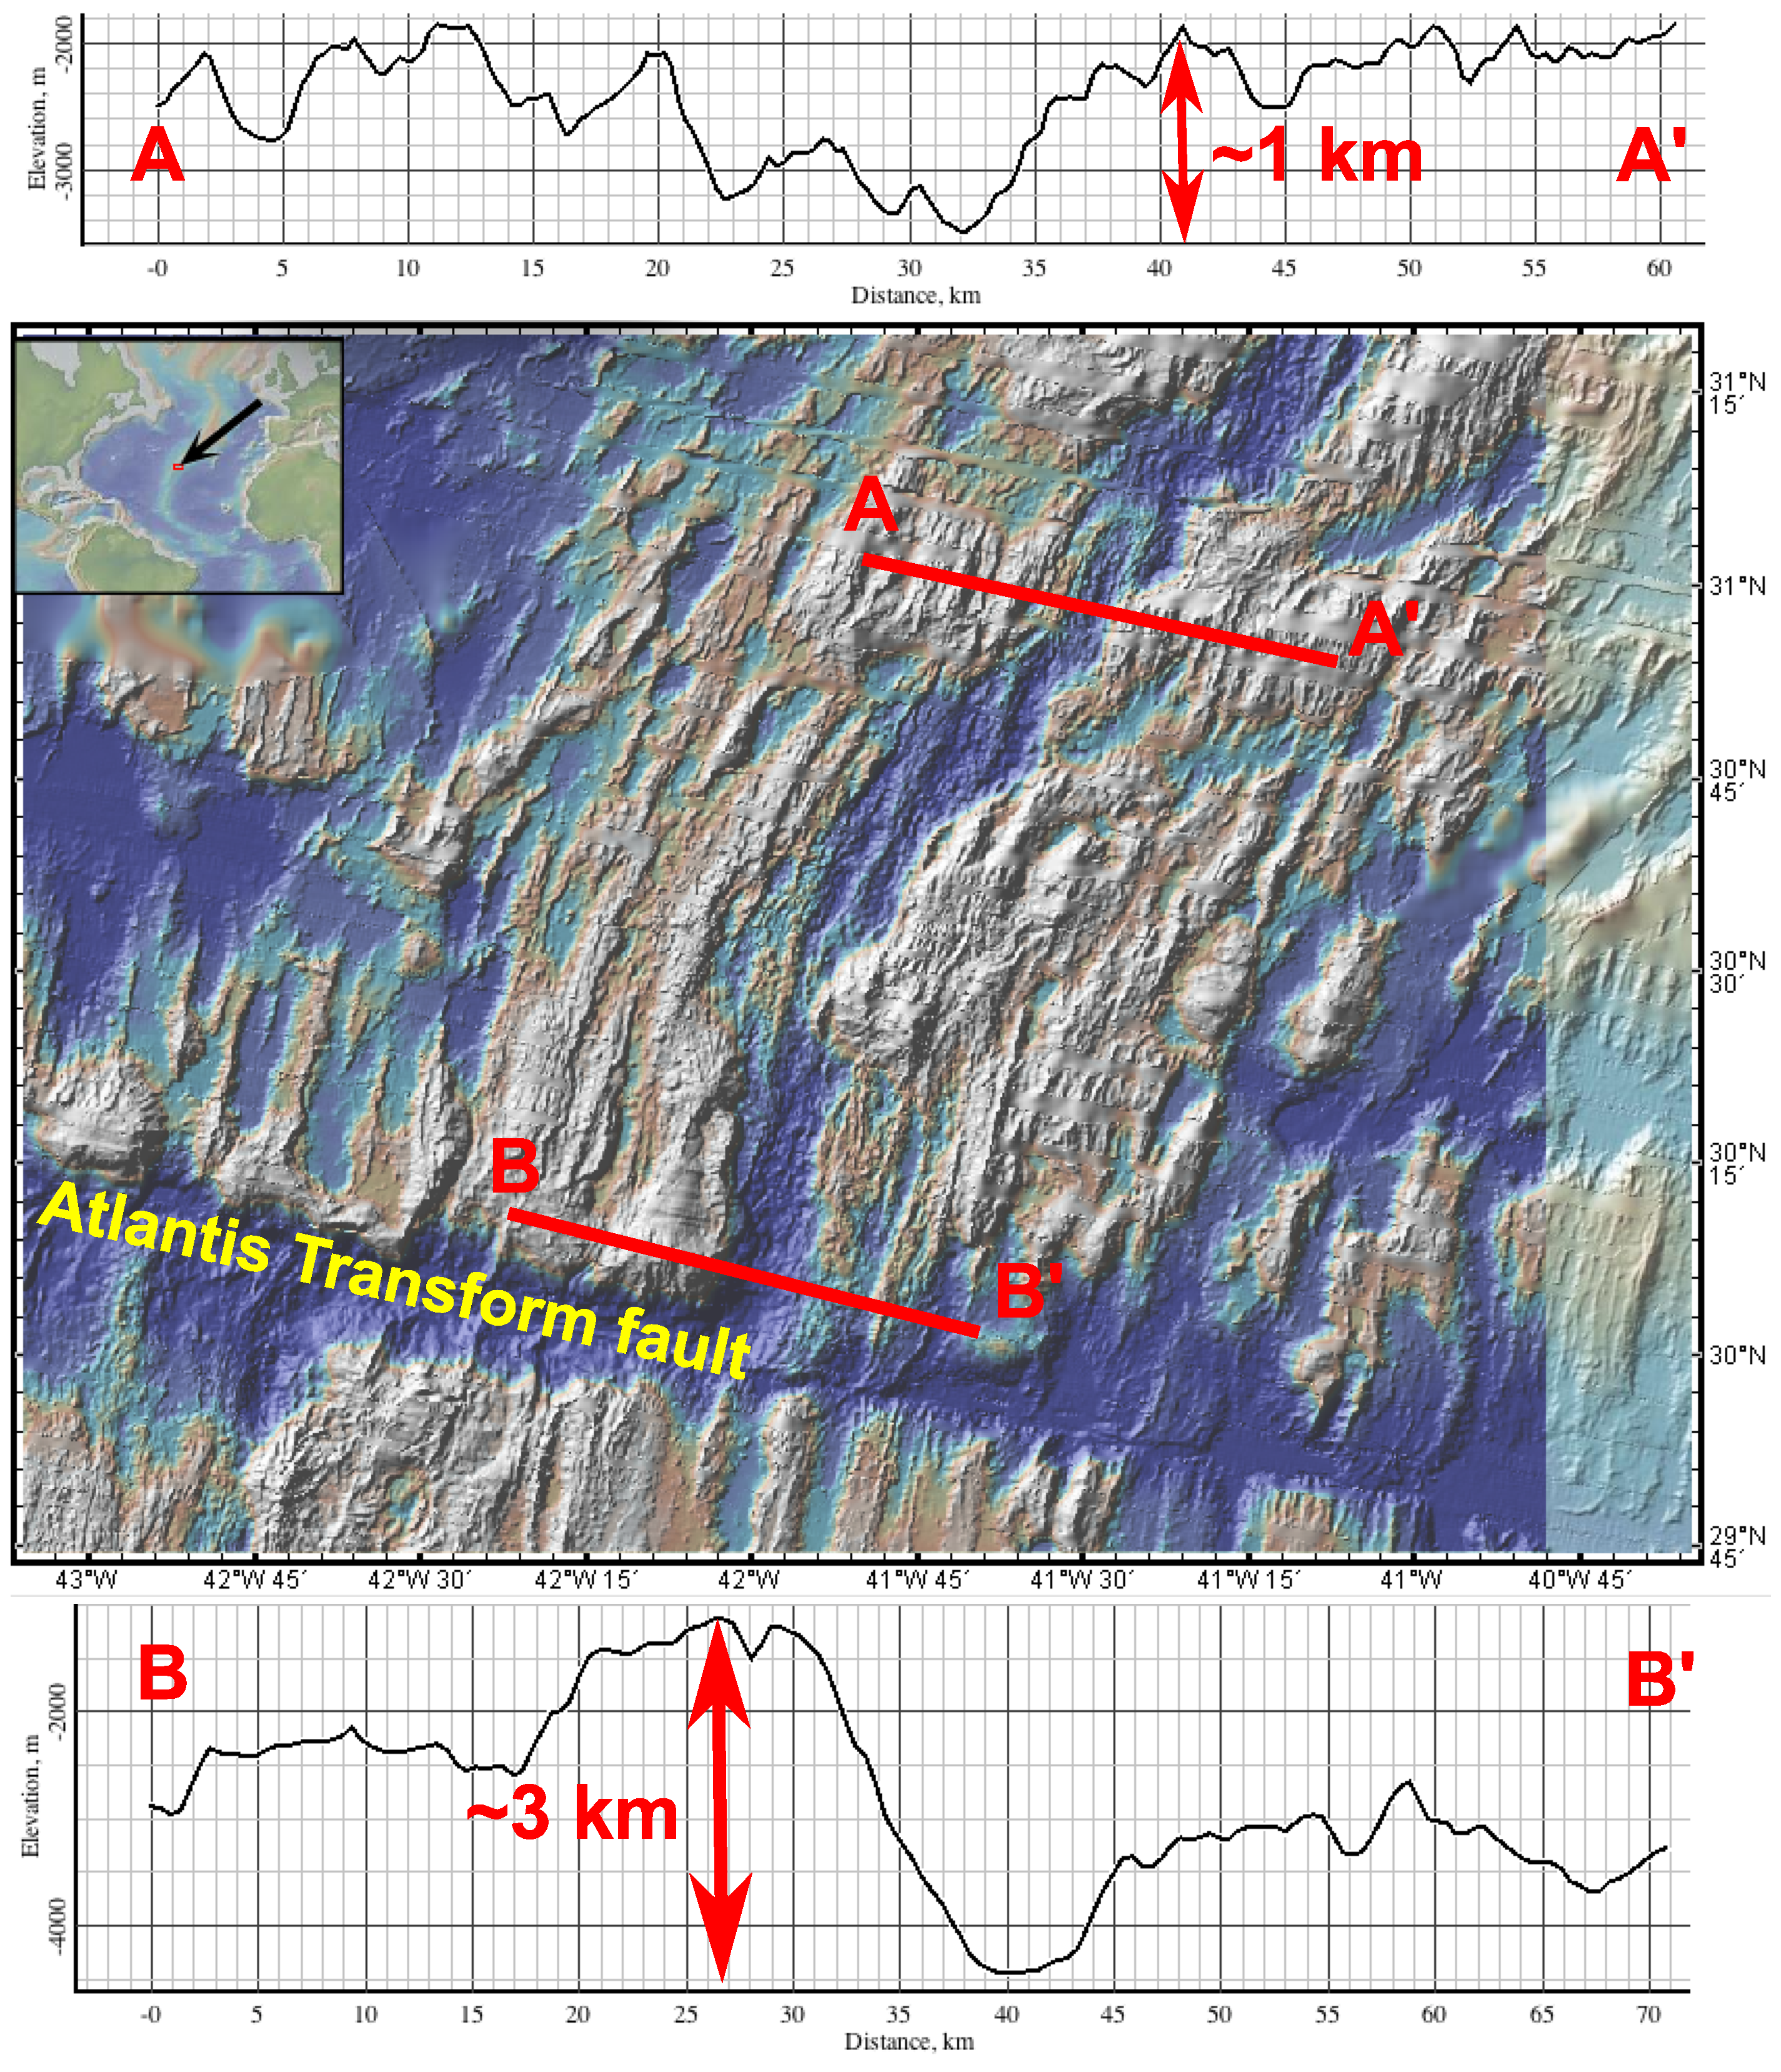
\includegraphics[width=0.65\textwidth]{./Figures/fig_Intro1_2_30N_MAR_offAxisMorphologies.eps}
 \caption[Two bathymetric profiles across the Mid-Atlantic Ridge around 30$\degree$N with vertical exaggeration of 10.]{Two bathymetric profiles across the Mid-Atlantic Ridge around 30$\degree$N with vertical exaggeration of 10. A-A$^{\prime}$ is closer to the segment center while B-B$^{\prime}$ is at the tip of the segment.}
  \label{fig_Intro2_1}
\end{figure}

\begin{figure}[H]
 \centering
  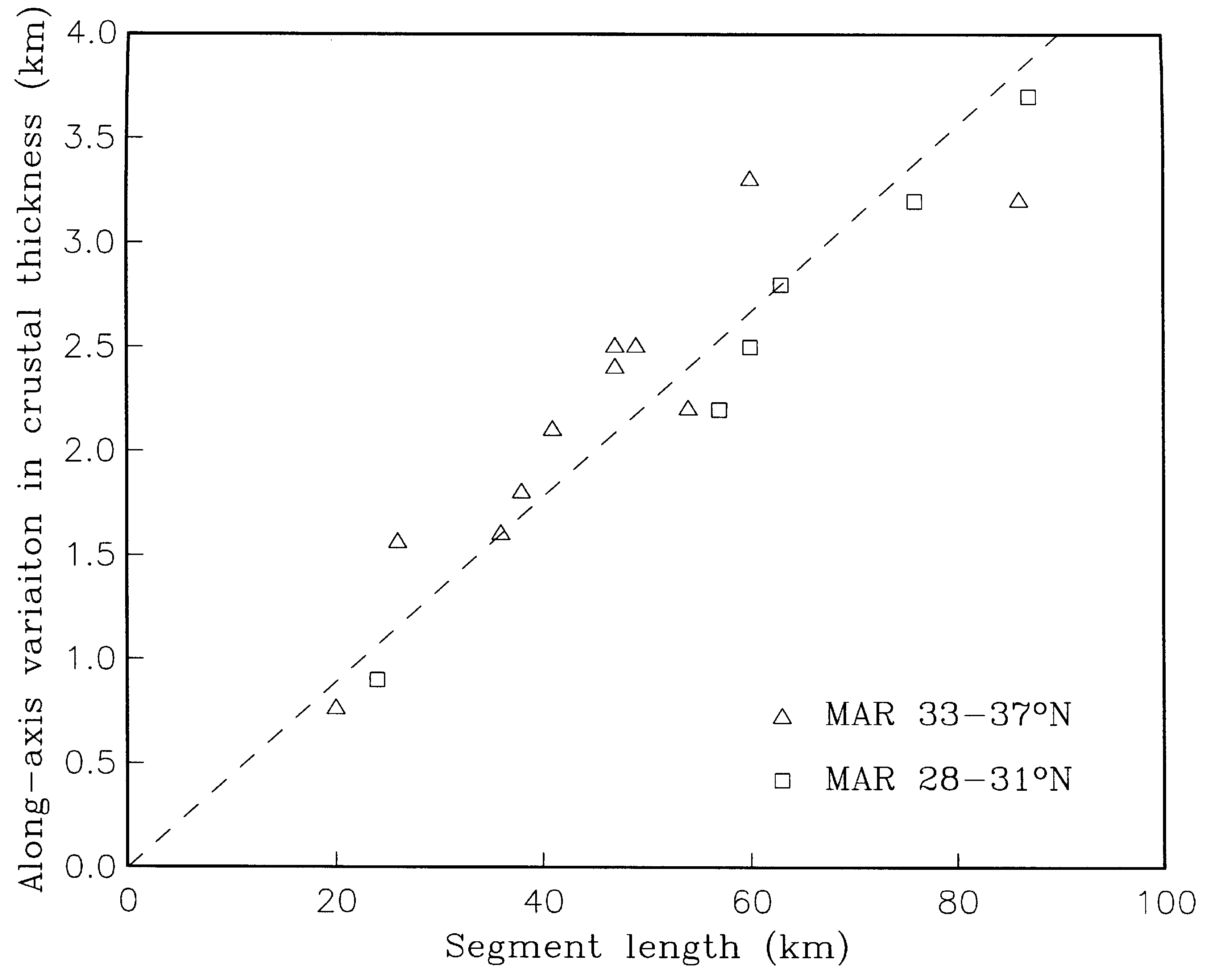
\includegraphics[width=0.5\textwidth]{./Figures/fig_Intro3_1.png}
 \caption[Relationship between the maximum crustal thickness variations ($\Delta H_{c}$) along a ridge segment and the segment length (L).]{Relationship between the maximum crustal thickness variations ($\Delta H_{c}$) along a ridge segment and the segment length (L). The dashed line is the best-fit linear regression of the combined data \citep{Chen1999}.}
 \label{fig_Intro3_1}
\end{figure}

%Moreover, a 3D view of B-B' area of Figure~\ref{fig2_1} shows the 20km wide, 25km long and 3km relief Atlantis Massif. The huge geologic structure is a window for learning lower crust and upper mantle because it is believed to be a result of exhumation of deeper material to the seafloor through tectonic processes.
%
%\begin{figure}[H]
% \centering
%  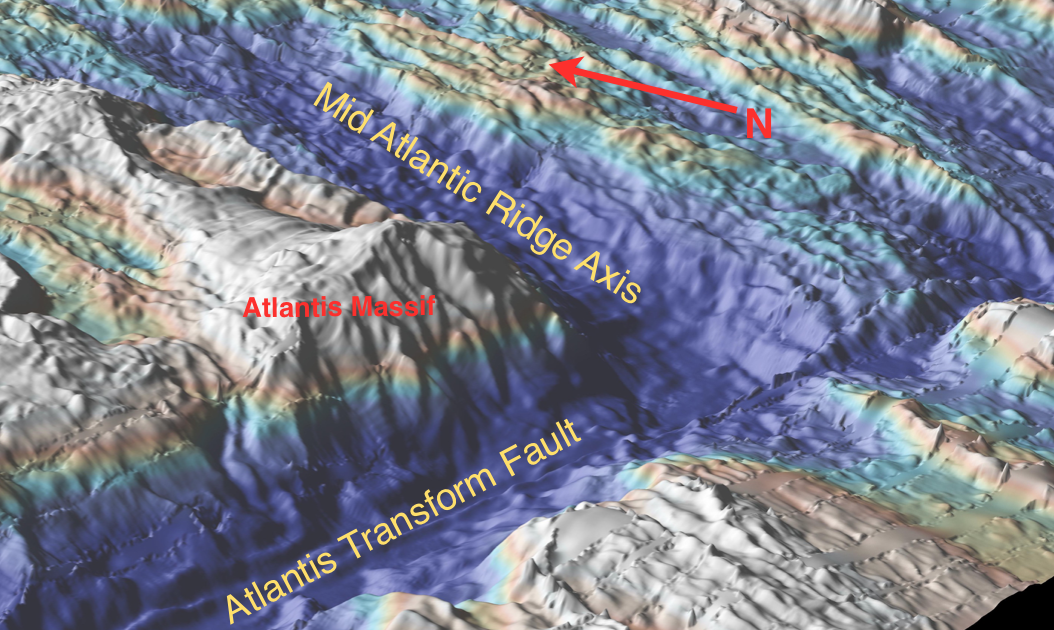
\includegraphics[scale=0.4]{fig4_1.png}
% \caption{\small{Zoom in B-B' area, a 3D view of Atlantis Massif.}}
% \label{fig4_1}
%\end{figure}

%\subsection{Related work}
%\label{ch:related}
Magma supply at the MORs is mostly a passive process when no hot plume is present \citep{Fowler2004}. Driven by both vertical pressure difference and buoyancy due to horizontal density difference, hot mantle rises up to fill the vacated room produced by the plate separation. Decompression of the upwelling hot mantle results in partial melting. The generated magma upwells to the upper crust and feeds the dikes at the ridge center. %Diking releases extensional stresses resulting from the extension forces (e.g slab pull, viscous mantle drag) that drive the seafloor spreading.

The passive nature of the melting process at the MORs leads to the major difference between fast and slow spreading ridges. At fast spreading ridges, magma is generated at a higher rate than at slow spreading ridges. Thus, fast spreading ridges experience more frequent diking, which efficiently releases stresses generated by far-field forces that drives the plate motion. In contrast, diking is less frequent at slow spreading ridges and can only partially release the stresses associated with plate motion. Thus, the brittle lithosphere of slow-spreading ridges experiences internal deformations (e.g., tectonic processes like normal faulting) when the deviatoric stress exceeds the internal strength of the lithosphere.

%For these reasons, the interactions between the deformation of oceanic lithosphere and the magmatism along the MORs have been carefully studied \citep[e.g.,][]{Buck2005, Tucholke2008}.

\citet{Buck2005} %attributed the contrasting faulting patterns and ocean floor morphology of fast- and slow-spreading ridges to the difference in the amount of diking-accommodated plate extension. They 
defined the ratio between the rates of dike widening and plate separation as M = $V_{dx}/2V_{x}$, where $V_{dx}$ is the rate of horizontally opening by diking at the ridge center and $V_{x}$ is the half spreading rate of the MOR. According to this definition, M = 1 represents the case where dike injection is so frequent that magma supply is sufficient to release all the tensional stresses from plate separation. M = 0 corresponds to the case of no magma supply, in which diking does not account for any of the plate motion and therefore plates kinematics requires plates to go through internal deformations. As shown in Figure~\ref{fig_Intro5_1}, an axial high forms at a fast spreading ridge (M = 1) due to buoyancy from lateral density difference across ridge axis but a median valley forms at a slow-spreading ridge (M = 0.5) due to near-axis normal faulting, which is in turn caused by the stretching of oceanic lithosphere.

%\citet[Buck2005}
%\annote[XT]{They didn't explicitly mention the ratio M, and they cannot remesh (the dike is not repeatedly widening), the dike in Poliakov and Buck is a vertical place where initial shear stress is set to zero and normal stress is set to be the same as lithostatic pressure, I guess it is still different with the following M we are going to describe, maybe Buck, 2005 is the first work to explicitly proposed M} {\note[EC]{I think M factor was originally proposed by Poliakov and Buck, 1998} }also showed that the ratio of the diking-accommodated portion to the total plate motion can efficiently parameterize the kinematics of repeated diking.}

\begin{figure}[h]
 \centering
  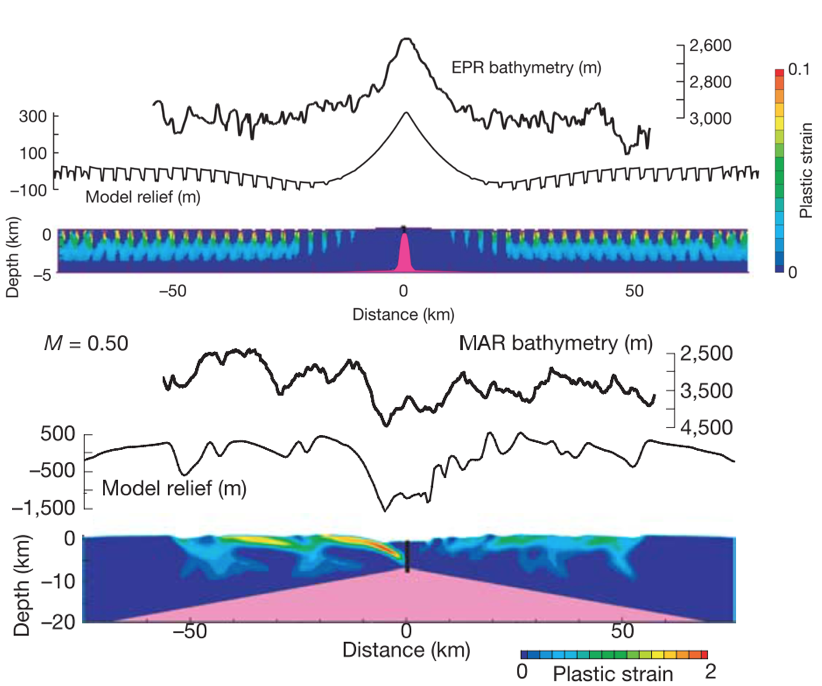
\includegraphics[width=0.8\textwidth]{./Figures/fig_Intro5_1.png}
 \caption[2D model results adapted from \citep{Buck2005}.]{Upper: modeling result for fast spreading agrees well with East Pacific Rise. Lower: modeling result for slow spreading ridges agrees well with the bathymetry of Mid-Atlantic Ridge. Adapted from \citep{Buck2005}.}
 \label{fig_Intro5_1}
\end{figure}

\citet{Tucholke2008} expand the investigation on the role of M in mid-ocean ridge mechanics. They focus on the faulting behaviors of slow spreading ridges and find that the OCCs are most likely to form when M varies from 0.3 to 0.5. When M = 0.7 (Fig.~\ref{fig_Intro6_1}), repeated diking pushes faults that have formed at the spreading center away from the ridge axis. Since the thickness of the brittle layer increases away from the ridge axis due to cooling effects, frictional and bending energy for maintaining the fault also increases. When the energy needed for maintaining an existing fault exceeds the energy for breaking a new near-axis fault, the old fault is replaced by the new one and most of the extension is accommodated by the new fault. When M = 0.3$\sim$0.5, the normal fault remains active for a long time and rotates to a low angle normal fault (detachment fault), exhuming the lower crust and mantle materials to the seafloor. When M $<$ 0.3, most of the tension is accommodated by intra-plate deformations rather than by diking and as a result, faulting pattern is more complicated and unsteady.

\begin{figure}[h]
 \centering
  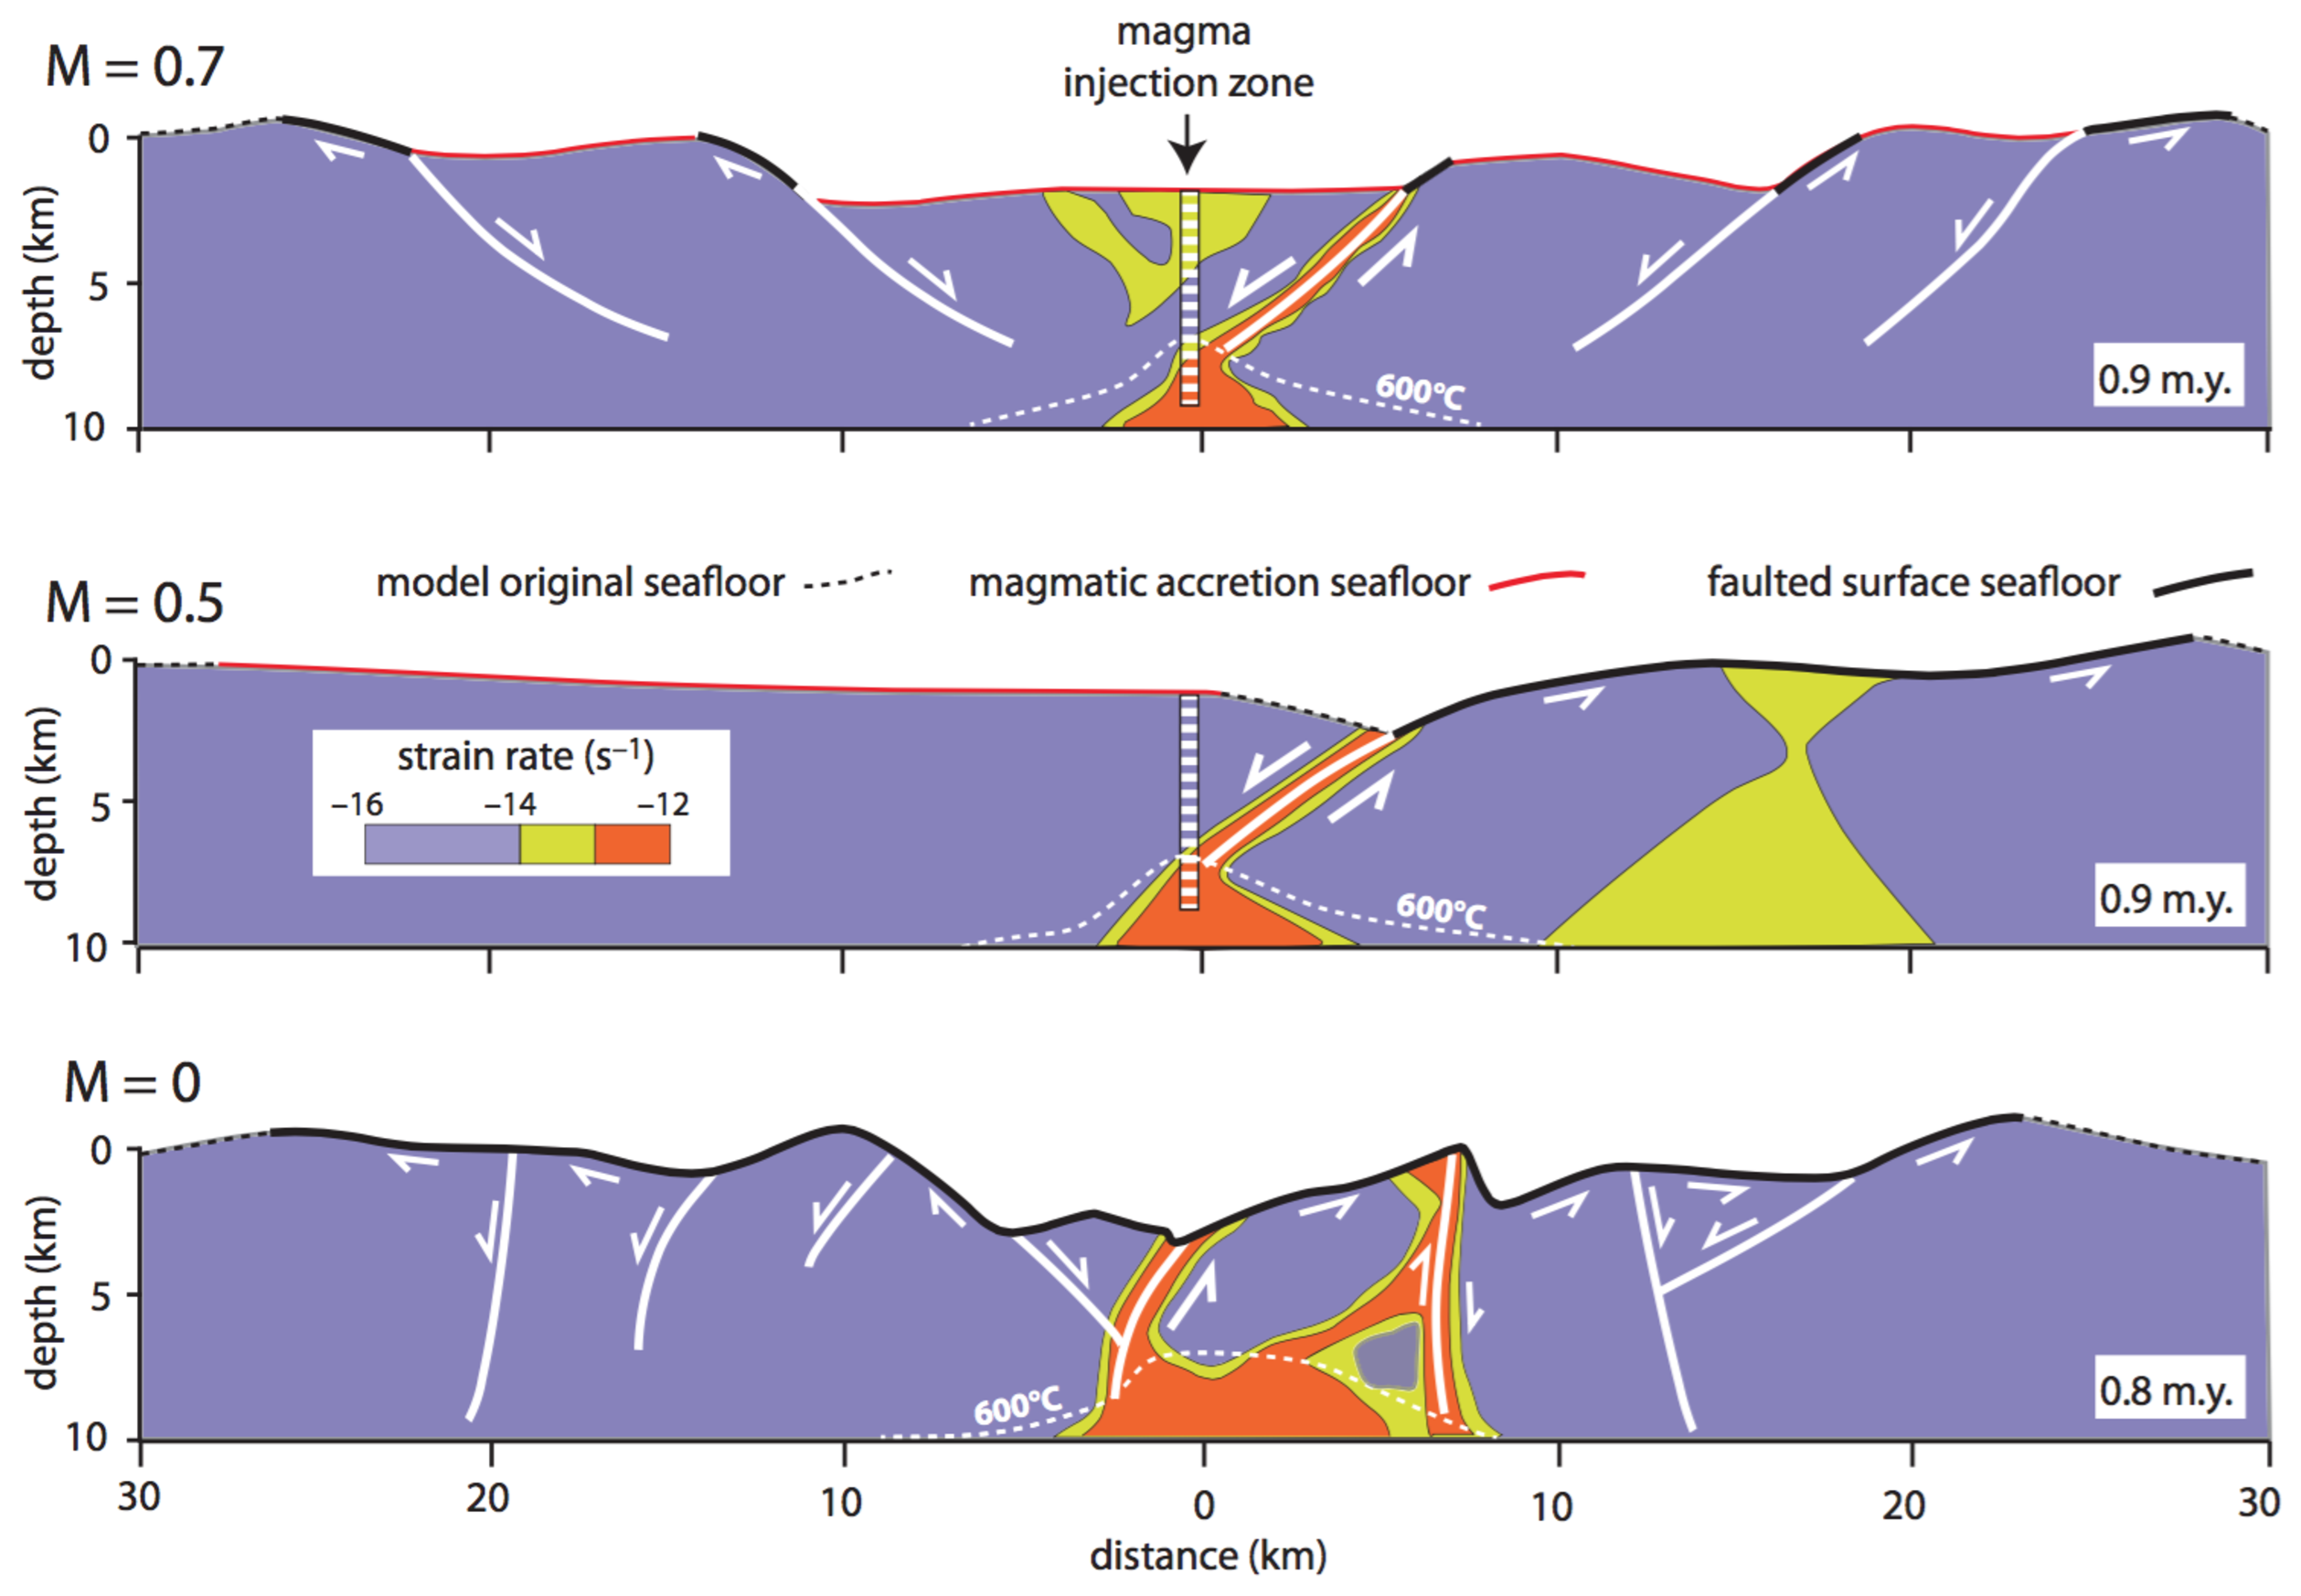
\includegraphics[width=0.8\textwidth]{./Figures/fig_Intro_Tucholke2008.eps}
 \caption[2D model results adapted from \citep{Tucholke2008,Whitney2012}.]{Snapshots of modeled fault behavior and seafloor morphology for M $=$ 0, 0.5, and 0.7; model allows thermal evolution. Structural interpretation is superimposed on modeled distribution of strain rate; model time is indicated in panels at lower right; dashed white line at bottom is 600 $\degree$C isotherm and approximates the brittle-ductile transition; dashed seafloor is original model seafloor, red seafloor is that formed dominantly by magmatic accretion, and solid bold seafloor is fault surface. Adapted from [\citealp{Tucholke2008,Whitney2012}]}.
 \label{fig_Intro6_1}
\end{figure}

\iffalse
\begin{figure}[H]
\floatbox[{\capbeside\thisfloatsetup{capbesideposition={right,bottom},capbesidewidth=5cm}}]{figure}[\FBwidth]
{\caption{\small A$\sim$F: Faulting behaviors for different values of M. Geologic interpretation is superimposed on modeled distribution of strain rate. Dots show breakaways of initial faults. Dashed seafloor is original model seafloor, red dotted seafloor is formed dominantly by magmatic accretion, and solid bold is fault surface. Note that the detachment faults in B and C are not interrupted by secondary faults. \citep{Tucholke2008}}}
 {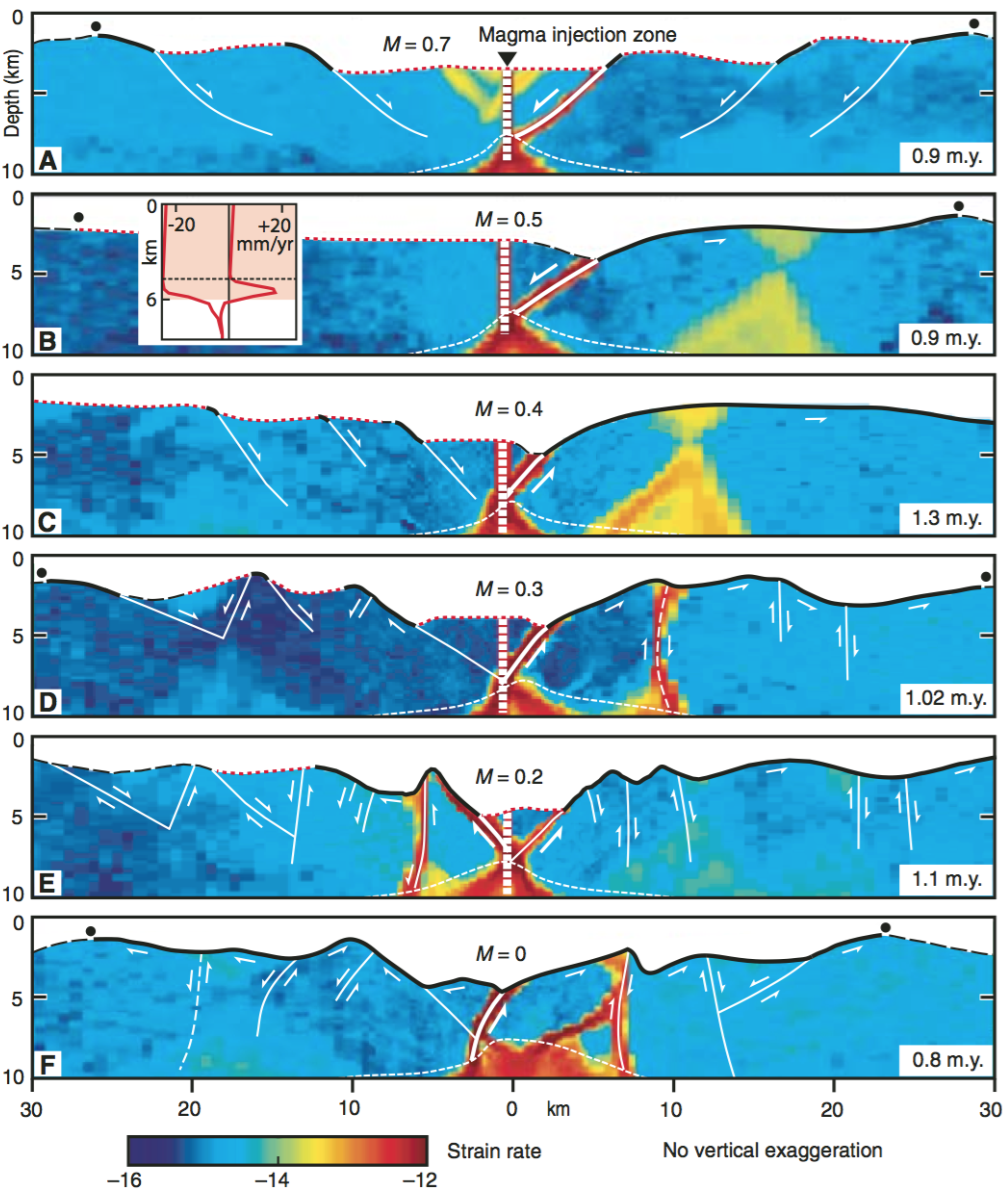
\includegraphics[width=10cm]{./Figures/fig_Intro6_1.png}} 
 \label{fig_Intro6_1}
\end{figure}
\fi
%\note[EC]{In the publication we will be writing, you'll also need to mention the works by Ito and Behn and Olive et al.}

\subsection{Statement of Research Purpose}

The M-factor formulation used in the previous 2D models \citep[e.g.,][]{Buck2005,Tucholke2008} successfully explained major features found in across-ridge profiles of seafloor bathymetry. However, 2D models have limitations in studying the along-ridge variations in morphology and faulting patterns. Magma supply at fast spreading ridges seems always sufficient for accommodating plate motions with little variations along the ridge axis. The relatively uniform topography along fast spreading ridges is considered to be consistent with the uniform abundance of the magma supply. However, along the slow spreading ridges, bathymetry, gravity anomaly and results from reflection and refraction seismology show strong correlation with variations in crustal thickness \citep[e.g.,][]{Lin1990, Tolstoy1993, Chen1999, Ryan2009}. Because oceanic crust is mainly formed by upwelling magma at the ridge center, variation in the thickness of the crust implies variation in magma supply. At slow spreading ridges, the degree of cooling by hydrothermal circulation, thermal structures and even local spreading rate \citep{Baines2008} also vary both along and across the ridge axis and they appear interrelated. Thus, for slow-to-intermediate spreading ridges, the interactions between tectonics and magmatism at MORs are inevitably 3D processes and 3D numerical models are desirable for investigating the factors that controls both across- and along-ridge morphology variations. 

The purpose of this thesis is to extend the M-factor formulation originally developed for 2D models to 3D by implementing it into a 3D numerical modeling code SNAC % (\textbf{S}tGermai\textbf{N} \textbf{A}nalysis of \textbf{C}ontinua)
\citep{Choi2008}. By systematically exploring the behaviors of the 3D models and comparing them with observations, we aim to better understand how the along-axis variation in diking at slow-to-intermediate mid-ocean ridges is responsible for the observed morphologies.

%\subsection{Findings}

\pagebreak
\section{Methods}
\label{ch:Methods}

\subsection{Method of approach}
The numerical modeling code, SNAC (\textbf{S}tGermai\textbf{N} \textbf{A}nalysis of \textbf{C}ontinua), is an explicit Lagrangian finite element code that solves the force and energy \add[XT]{find out which one is energy balance equation} balance equations for elasto-visco-plastic materials. Figure~\ref{fig_Methods7_3} shows major components of SNAC.

For each time step, strain and strain rates are updated based on the initial or previous velocity fields under the constraints from boundary conditions. A constitutive model returns updated stresses corresponding to these deformation measures. Internal forces are then calculated from the updated stresses, which is plugged into the momentum balance equation together with the body force term. Then, the damped \add[XT]{better understand the damped force} net force divided by inertial mass yields acceleration at a node point, which is time-integrated to velocity and displacement.

A 3D domain is discretized into hexahedral elements, each of which is in turn divided into two sets of tetrahedra. This symmetric discretization prevents faulting from favoring a specific direction or ``mesh grains''. 

Rheology for the oceanic lithosphere is assumed to be elasto-visco-plastic (EVP). When viscosity is high at low temperature, the EVP rheology implemented in SNAC essentially becomes the Mohr-Coulomb plasticity with strain softening that can create shear bands that behave like faults. Strain softening is realized by cohesion decreasing with increasing amount of permanent (i.e., plastic) strain. I assume this relationship is linear for simplicity. It is sufficient for a full description of such a linear strain weakening to define initial and final values of cohesion and a critical plastic strain at which cohesion becomes the final value. I define the rate of strain weakening as the cohesion difference divided by the critical plastic strain and use it as one of the model parameters. When temperature is high and viscosity is low, the rheology becomes the Maxwell viscoelasticity and can model creeping flow. This property of the EVP model makes it possible to set up a structure with a brittle lithosphere and a ductile asthenosphere through a proper temperature distribution. Rheological parameters are taken from previous studies that use a similar rheology [e.g., \citealp{Buck2005}; \citealp{Tucholke2008}] or from lab experiments \citep[e.g.,][]{Kirby1987}. 

For 3D diking processs, the strain $\Delta\varepsilon_{xx}$ associated with diking leads to stresses changes, $\Delta\sigma_{xx}$, $\Delta\sigma_{yy}$ and $\Delta\sigma_{zz}$. These stress changes due to diking are computed according to the linear elastic constitutive equations $\sigma_{ij}=\lambda\varepsilon_{kk}\delta_{ij}+2\mu\varepsilon_{ij}$.

\begin{figure}[H]
 \centering
%  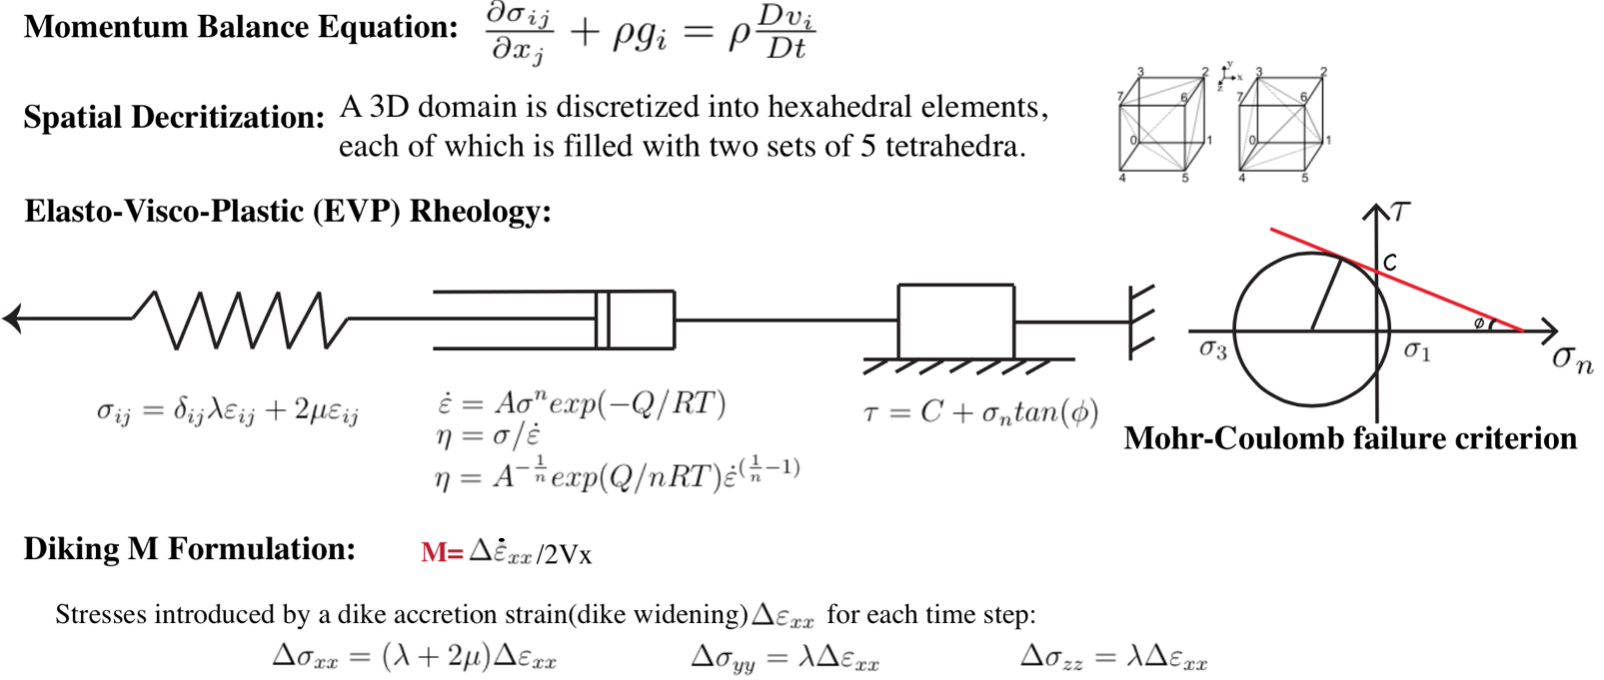
\includegraphics[scale=0.65]{fig_Methods7_2.png}
  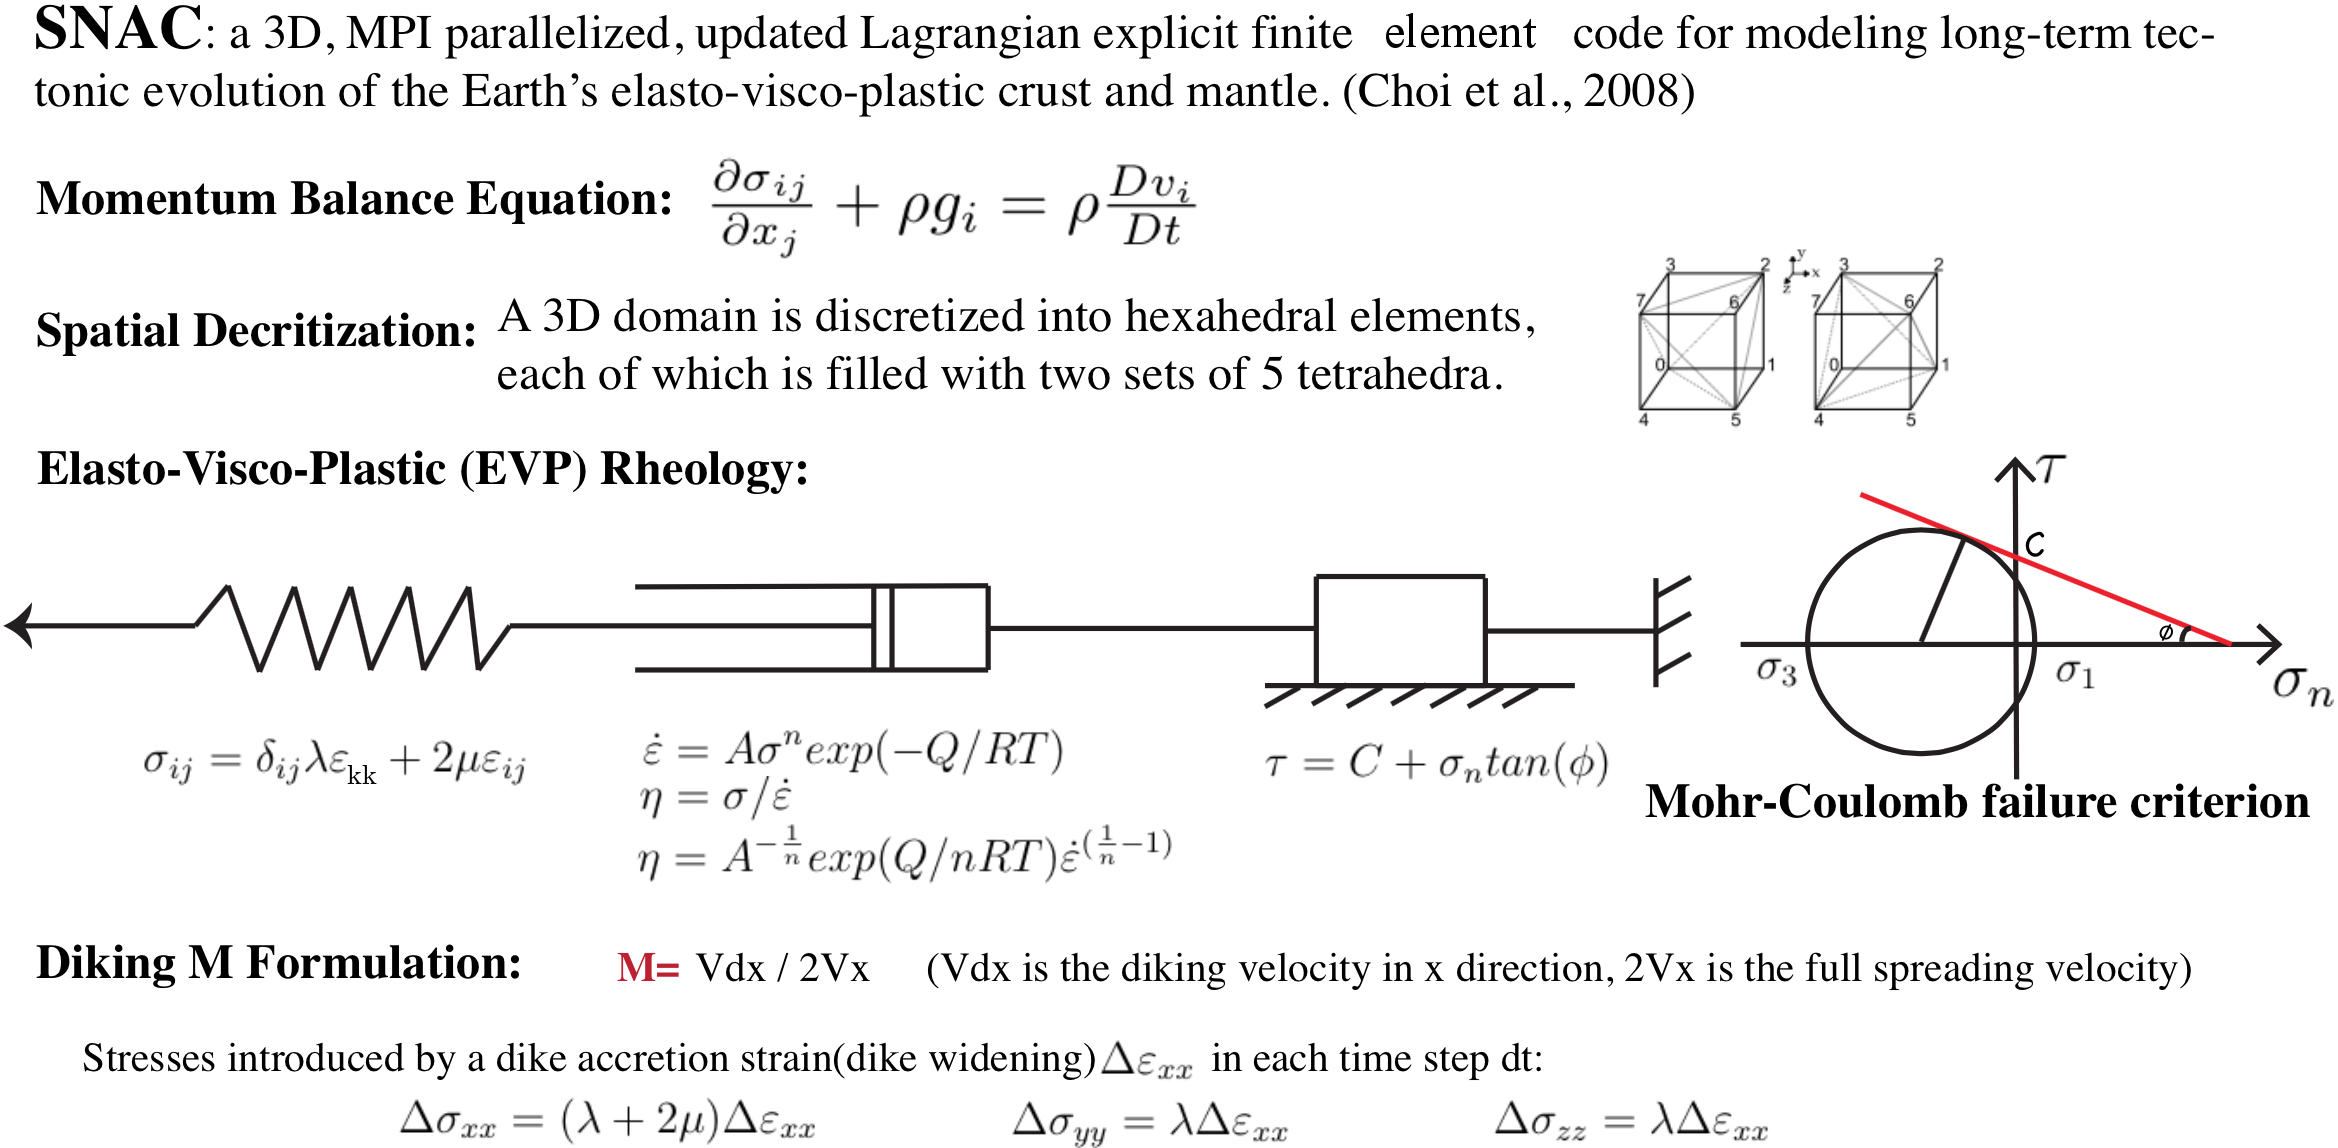
\includegraphics[width=1.0\textwidth]{./Figures/fig_Methods7_3.png}
 \caption{\small{Essential components of the numerical method.}}
 \label{fig_Methods7_3}
\end{figure}

\subsection{Model Setup}
The 3D models have a common geometry of 60 km $\times$ 20 km $\times$ 20 km in $x$, $y$ and $z$ axes respectively with a resolution ($\Delta x$) of 1 km (i.e., $\Delta x$ is the size of each hexahedron element). %For comparison with the previous 2D models \citep[e.g.][]{Buck2005, Tucholke2008}, I \note[EC]{also run pseudo-2D models}{Are you still going to include pseudo-2D models?} and they have a geometry of (60 km $\times$ 20 km $\times$ 1 km) in $x$, $y$ and $z$ axes respectively with a resolution of $\Delta x$ = 0.5 km.
The initial temperature field linearly increases from 0 \degree C at the top surface to 240 \degree C at the depth of 6 km, reflecting enhanced cooling due to hydrothermal circulation (Fig.~\ref{fig_Methods8_1}). Below 6 km, the temperature profile follows the semi-infinite half-space cooling model of moving plates \citep[e.g.,][]{Turcotte2002}. Two sides perpendicular to the $z$ coordinate axis are free-slip. The top surface has vertical tractions from water columns, of which heights are locally determined as (4000 - $h(x,z)$) m, where $h(x,z)$ is the topography at a location, $(x,z)$. The bottom surface is supported by the Winkler foundation. Temperature is fixed at 0 \degree C on the top surface and at 1300 \degree C on the bottom surface. 

Diking, represented by the factor M as described above, is assumed to occur in the middle of the doamin (Fig.~\ref{fig_Methods8_1}), where the lithosphere is the thinnest.

We adopt the linear isotropic elasticity, power-law viscosity of dry diabase \citep[e.g.,][]{Kirby1987, Buck2005} and the Mohr-Coulomb plastic model. The complete list of model parameters are given in Table~\hyperref[Tab_ModelParameters]{\ref{Tab_ModelParameters}}.

\begin{figure}[h]
 \centering
  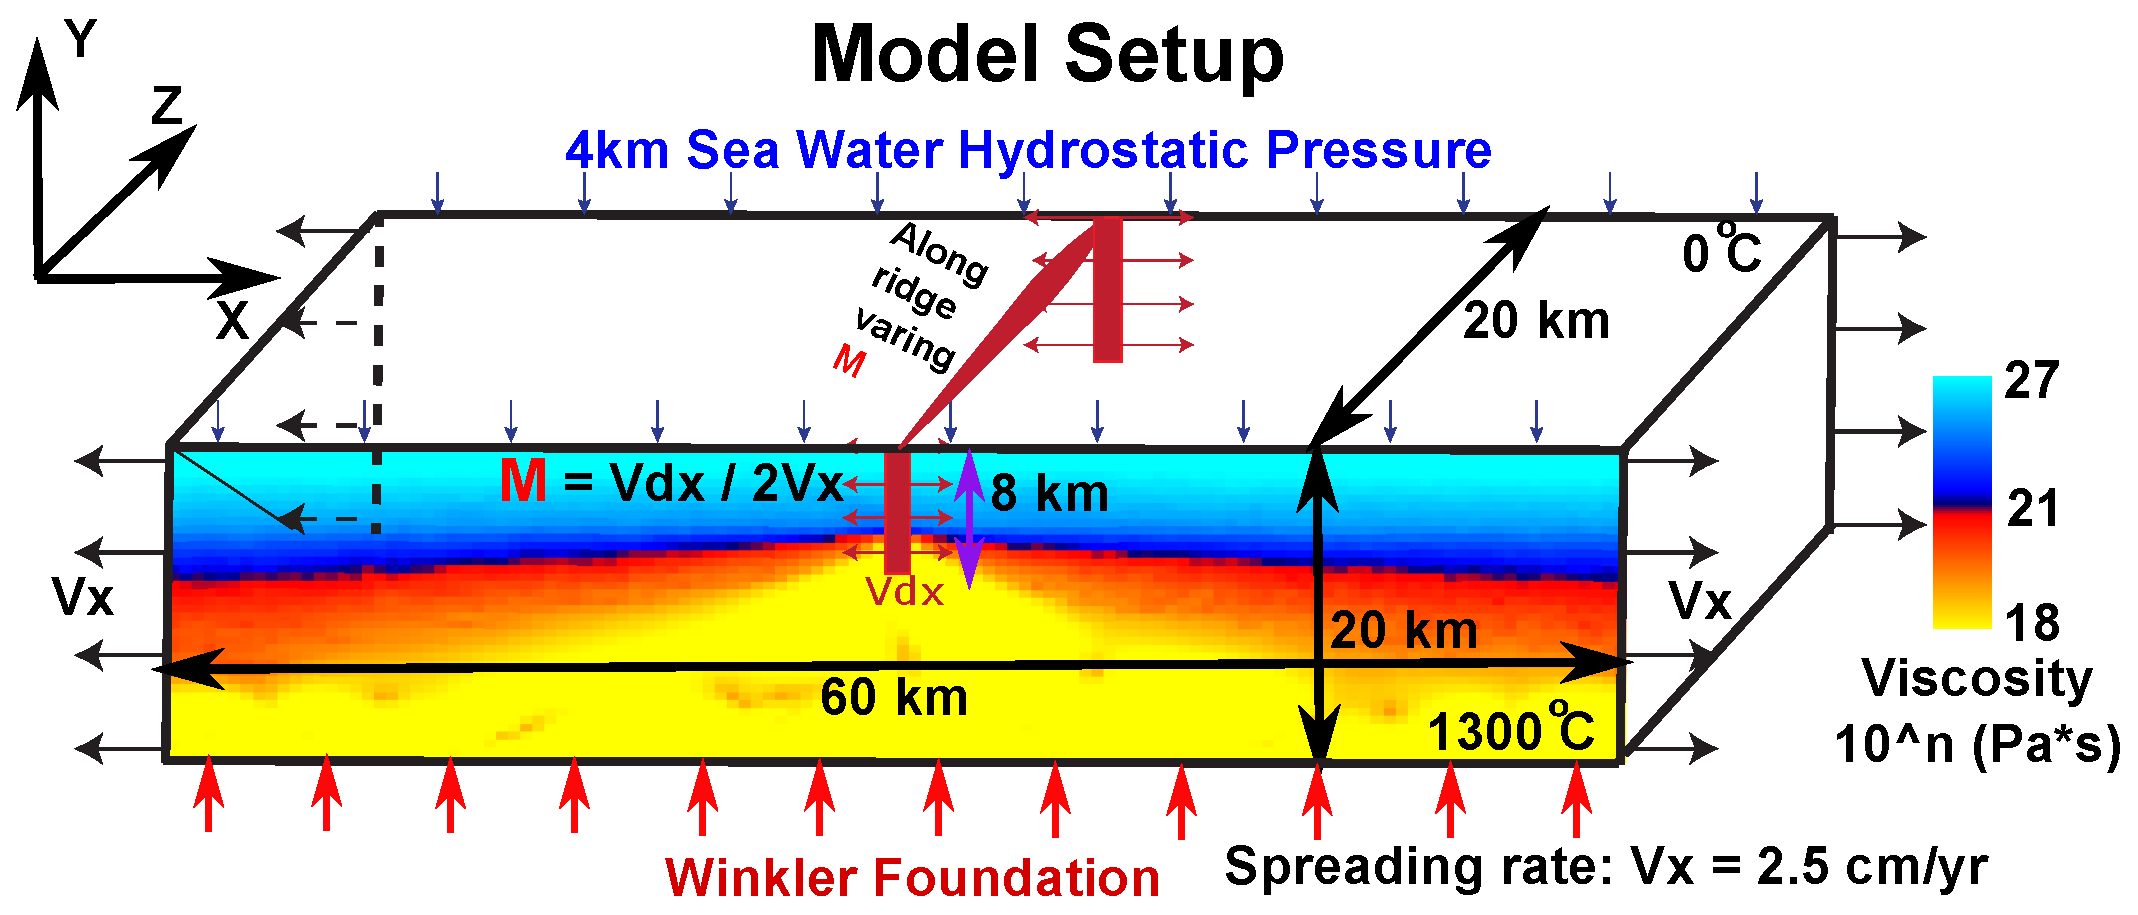
\includegraphics[width=1.0\textwidth] {./Figures/fig_Methods_Model_Setup.eps}
 \caption{\small Model setup}
 \label{fig_Methods8_1}
\end{figure}

\begin{table}[h]
\caption{Summary of 3D Model Parameters}
\centering
 \small
  \begin{tabular}[h]{l l p{6.8cm} l l}
\hline
\hline
Number & Variable & Description & Value & Units \\ 
\hline
1    &  $W_{dike}$    &   Dike width        & 2   &  $km$\\
\hline
2    &  $D_{dike}$    &   Dike depth        & 8   &  $km$\\
\hline
3    &  $H$    &   Crustal thickness at dike   & 6   &  $km$ \\
\hline
4    &  $dT/dy$    &   Crustal thermal gradient        & 40   &  $K/km$ \\
\hline
5    &  $T_{1}$    &   Temperature at lower boundary of crust    & 240   &  $\degree C$ \\
\hline
6    &  $g$    &   Gravity acceleration    & 10   &  $m/s^{2}$ \\
\hline
7    &  $demf$    &   Dimensionless force damping factor   & 0.8   &  N/A  \\
\hline
8    &  $dt$    &   Time step    & 1.5768e+07   &  $second$  \\
\hline
9    &  $topo_kappa$    &   Parameter for topography smoothing    & 0   &  N/A   \\
\hline
10   &  $shadowDepth$    &   Ghost elements for parallel computing   & 2   &  N/A   \\
\hline
11   &  $meshI$    &   Mesh number in X direction   & 60   &  N/A   \\
\hline
12   &  $meshJ$    &   Mesh number in Y direction      & 20   & N/A  \\
\hline
13   &  $meshK$    &   Mesh number in Z direction      & 20   & N/A  \\
\hline
14   &  $L_{I}$    &   Length in X direction      & 20   & $km$  \\
\hline
15   &  $L_{J}$    &   Length in Y direction      & 20   & $km$  \\
\hline
16   &  $L_{K}$    &   Length in Z direction      & 20   & $km$  \\
\hline
17   &  $\rho$    &    Density      & 3000   & $kg/m^{3}$  \\
\hline
18   &  $\lambda$    &    Lam$\acute{e}$'s constant      & 30   & $Gpa$  \\
\hline
19   &  $\mu$    &    Shear modulus      & 30   & $Gpa$  \\
\hline
20   &  $refvisc$    &    Reference viscosity      & 0.125e-17   & $Pa^{-n}/s$  \\
\hline
21   &  $activationE$    &    Activation Energy      & 276.0e+3   & $kJ/mol$  \\
\hline
22   &  $vis_{min}$    &    viscosity minimum cutoff      & 1.0e+18   & $Pa*s$  \\
\hline
23   &  $vis_{max}$    &    viscosity maximum cutoff      & 1.0e+27   & $Pa*s$  \\
\hline
24   &  $srexponent$    &    Power of power law in viscosity       & 3.05   & N/A  \\
\hline
25   &  $\varepsilon_{p_{i}}^{1}$    &    initial plastic strain for piecewise Type 1 weakening       & $0$   & N/A  \\
\hline
26   &  $\varepsilon_{p_{i}}^{2}$    &    initial plastic strain for piecewise Type 2 weakening       & $0$   & N/A  \\
\hline
27   &  $\varepsilon_{p_{e}}^{1}$    &    end plastic strain for piecewise Type 1 weakening       & $0.1$   & N/A  \\
\hline
28   &  $\varepsilon_{p_{e}}^{2}$    &    end plastic strain for piecewise Type 2 weakening       & $0.33$   & N/A  \\
\hline
29   &  $C_{i}$    &    initial Cohesion for piecewise weakening       & 44   & $Mpa$  \\
\hline
30   &  $C_{e}$    &    end Cohesion for piecewise weakening       & 4   & $Mpa$  \\
\hline
31   &  $\phi$    &    Friction angle      & 30   & $\degree$  \\
\hline
32   &  $remesh_{timestep}$    &    Remesh when timestep reach its value      & 400000   & N/A  \\
\hline
33   &  $remesh_{length}$    &    Remesh when the global minimum of the ratio of the volume of a tetrahedron to one of its surface area      & 0.6   & N/A  \\
\hline
34   &  $top_{Temp}$    &    Surface temperature      & 0   & $\degree C$  \\
\hline
35   &  $bottom_{Temp}$    &    Bottom temperature      & 1300   & $\degree C$  \\
\hline
36   &  $V_{x}$    &    Half spreading rate      & 7.9e-10   & $m/s$  \\

\hline
\hline
\end{tabular}

\label{Tab_ModelParameters}
\end{table}

\subsection{Parameters to control}
Before running 3D models, I have run hundreds of psedudo-2D models for initial setup and benchmarking with previous studies \citep[e.g.,][]{Buck2005, Tucholke2008}. Preliminary pseudo-2D results show that the model behavior in faulting pattern is sensitive to the rate of strain weakening. Two cases of strain weakening are tested in the 3D models. In one case (denoted as Type 1 weakening), cohesion linearly decreases from 44 MPa (denoted as $C_{i}$) to 4 MPa ($C_{e}$) for plastic strain accumulating from 0 ($\varepsilon_{p_{i}}^{1}$) to 0.1 ($\varepsilon_{p_{e}}^{1}$). It has a characteristic fault slip of 150 m for pseudo-2D models and 300 m for 3D models. The other case (Type 2 weakening) assumes cohesion linearly decreasing from 44 MPa ($C_{i}$) to 4 MPa ($C_{e}$) for plastic strain accumulating from 0 ($\varepsilon_{p_{i}}^{2}$) to 0.33 ($\varepsilon_{p_{e}}^{2}$). In this case, the characteristic fault slip for pseudo-2D models is 500 m and for 3D models is 1 km. The characteristic fault slip is defined as $\Delta X_{c}$=3$\Delta x \varepsilon_{p_{e}}$ where 3 $\Delta x$ represents the thickness of the shear bands which is usually 2 to 4 times $\Delta x$ (size of a hexahedron element) \citep{Lavier2000}. When $\Delta X_{c}$ amount of slip takes place at the fault interface, the cohesion of the material at the faulting interface decreases to $C_{e}$. In this way, under the same amount of $\Delta X_{c}$, models with different resolution should produce the same faulting patterns. 

Meanwhile, although how to estimate the M values from observations is a subject of on-going research, we do have constraints from a large dataset of bathymetry, gravity and seismic surveys as well as geological drilling. Generally, at slow spreading ridges, magma supplies mostly at the center of the ridge segment and decreases towards the tip of the segment \citep{Tolstoy1993,Chen1999,Carbotte2015}. There is also evidence for shorter wavelength of 10 to 20 km discrete focus of magma accretion along the ridge axis \citep{Lin1990}.

The numerical cost of a 3D model is non-trivial. For 2 Myr of model time, each model usually runs on 192 cores for about 48 hours (i.e., around 10$^{4}$ core-hours). %\add[XT]{use 96 cores can improve the efficiency a little bit (Longer time but smaller amount of SUs needed).})
Based on the observational and computational constraints, I start considering a few scenarios of variations in M along the ridge axis. They are 1) there types of functional forms (i.e. linear, sinusoidal and square root); 2) three ranges of M variation along the ridge axis (0.5$\sim$0.7 (M57); 0.5$\sim$0.8 (M58); 0.2$\sim$0.8 (M28)) and 3) two types of weakening rate (type 1 and type 2).

Till now, 11 $+$ 1 3D models are run (11 models with M varying along the ridge-axis and 1 model with constant M = 0.8. The complete list of 3D models is given in Table~\hyperref[Tab1_1]{\ref{Tab1_1}}. 

\begin{table}[h]
\centering
\begin{tabular}{l l l l l}
\hline
\hline
Model& M range & Functional Form & Type of weakening & For short \\ 
\hline
1    &  M28    &   Linear        & Type 1   &  M28LinT1\\
\hline
2    &  M28    &   Sinusoidal    & Type 1   &  M28SinT1\\
\hline
3    &  M28    &   Square Root   & Type 1   &  M28SqrtT1 \\
\hline
4    &  M57    &   Linear        & Type 1   &  M57LinT1 \\
\hline
5    &  M57    &   Sinusoidal    & Type 1   &  M57SinT1 \\
\hline
6    &  M57    &   Sinusoidal    & Type 2   &  M57SinT2 \\
\hline
7    &  M57    &   Square Root   & Type 2   &  M57SqrtT2  \\
\hline
8    &  M58    &   Sinusoidal    & Type 1   &  M58SinT1  \\
\hline
9    &  M58    &   Sinusoidal    & Type 2   &  M58SinT2   \\
\hline
10   &  M58    &   Square Root   & Type 1   &  M58SqrtT1   \\
\hline
11   &  M58    &   Square Root   & Type 2   &  M58SqrtT2   \\
\hline
12   &  M88    &   Constant      & Type 2   &  M88ConT2 \\
\hline
\hline
\end{tabular}
\caption{List of 3D numerical experiments.}
\label{Tab1_1}
\end{table}





\pagebreak
\section{3D Results}
\add[XT]{add one more section as an individual file/chapter for 2D models description.}
%\subsection{3D model results}
%\add[XT]{choose some points in the model domain like Choi 2008 did, to monitor the values changes with time (e.g. In VisIt use Query to obtain stress with time for quantatatively analyzing the model behaviors)}
Currently, we have three factors controlling the model behaviors. They are three ranges of M variation along the ridge axis (0.5$\sim$0.7; 0.5$\sim$0.8; 0.2$\sim$0.8), three functional forms of M variation (linear; sinusoidal; square root) and two types of weakening rate (Type one and Type two) as described in detail in the section ``Parameters to control''. 

In this ``Results'' chapter, we will first describe in detail the model behaviors of two reference models. Then, we will compare the reference model and the other data points with different setup parameters. %Formation mechanism will be explained mostly in this chapter and will be further discussed and compared with nature observation in the ``Discussion'' chapter. 

\subsection{Reference models (M28LinT1 Table~\hyperref[Tab1_1]{\ref{Tab1_1}})}\label{sec_M28LinT1}

We consider M varies linearly from 0.2 to 0.8 along the ridge axis with increasing Z as our reference model.

\begin{figure}[h]
  \centering
    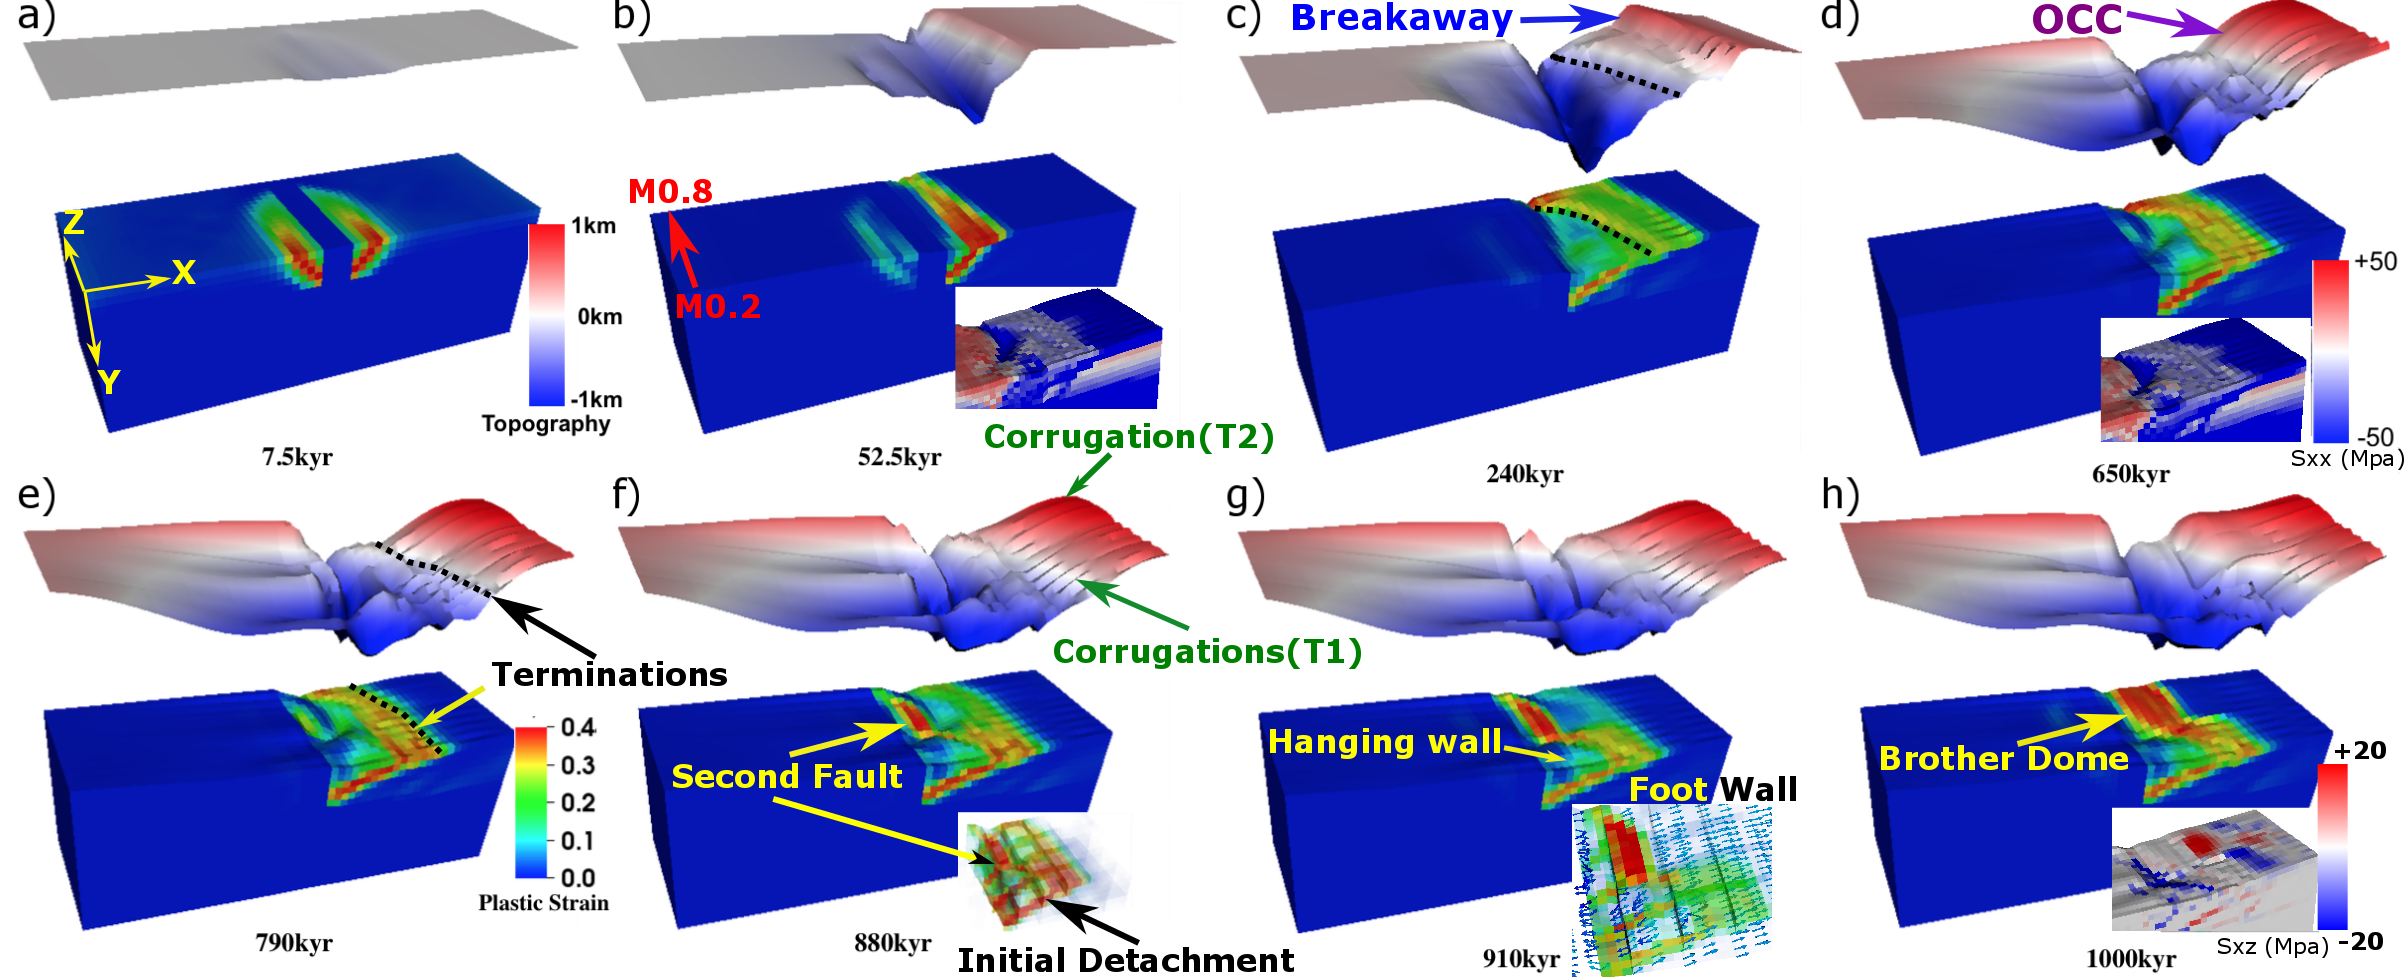
\includegraphics[width=1.0\textwidth]{./Figures/fig_Results1_1.png}
  \caption{Reference model one: M linearly increases from 0.2 to 0.8 from front to back, Type one weakening (M28LinT1) (Table~\hyperref[Tab1_1]{\ref{Tab1_1}}). The top layer is the topography of the model with five times vertical exaggeration. The color scale within Figure~\hyperref[fig_Results1_1]{\ref{fig_Results1_1}.a} is for the topography. Initial seafloor is marked as a reference of zero km in height.  The green, yellow and red colors in the background of blue model domain are plastic strain. Its color scale is shown in Figure~\hyperref[fig_Results1_1]{\ref{fig_Results1_1}.e}. The number with kyr as a unit beneath each model result is the time for the model with a unit of thousands of year. The two insets in Figure~\hyperref[fig_Results1_1]{\ref{fig_Results1_1}.b} and Figure~\hyperref[fig_Results1_1]{\ref{fig_Results1_1}.d} is for stress $\sigma_{xx}$ (Sxx in the figure). Positive value (pink and red) means tension and negative (blue) is compression. The inset in Figure~\hyperref[fig_Results1_1]{\ref{fig_Results1_1}.h} is for shear stress $\sigma_{xz}$ (Sxz in the figure). It share the same color scale with insets in the Figure~\hyperref[fig_Results1_1]{\ref{fig_Results1_1}.b} and Figure~\hyperref[fig_Results1_1]{\ref{fig_Results1_1}.d}. The inset in Figure~\hyperref[fig_Results1_1]{\ref{fig_Results1_1}.f} is a transparent view of plastic strain. The inset in Figure~\hyperref[fig_Results1_1]{\ref{fig_Results1_1}.g} shows both plastic strain and the velocity vector. Indicated by the velocity vector, the hanging wall of the detachment fault at low M region (M0.2$\sim$M0.5) is moving in an opposite direction to the hanging wall at higher M region (M$>0.5$).} %\note[XT]{one thing to be noted is that the $dt=0.5yr$ in these series of 3D models, thus I divided the time step by two to get the time (kyr). This figure needs to be revised that the plastic strain scale is actually changing for different time, a way to revise it is to maintain a constant color scale or attach a color scale for each time. Also, it seems a little bit small and two rows is not as preferable as one row or one column to better express the concept of linear time series evolution.}}
 \label{fig_Results1_1}
\end{figure}   

As shown in Figure~\hyperref[fig_Results1_1]{\ref{fig_Results1_1}}, the model creates a median valley that both widens and deepens through time and the rate of its widening and deepening at a specific location (in terms of Z-axis) is inverse proportional to the rate of local magma supply (i.e. M value). OCCs with more than one kilometer in relief and tens of kilometers in wavelentgh are produced in the model. One interesting behavior worth noting is that corrugations with hundred-to-kilometer wavelengths are also produced by the model.

As shown in Figure~\hyperref[fig_Results1_1]{\ref{fig_Results1_1}.a}, in the first 7.5kyr, high angle ($\sim 60 \degree$)(consistent with  Anderson's theory of faulting mechanics for a frictional angle of 30$\degree$) normal faults (shown as higher plastic strain shear bands with a thickness of 2$\sim$4 times of the width of a single hexahedron element) begin to form near the ridge axis in terms of plastic strain localization near the ridge center (weakest place to initiate a fault), because of the thickness of the crust is thinnest at the ridge center due to our thermal structure setup. For each timestep, the tensional stress accummulates faster at the lower M side where the crust reaches a yielding point earlier than higher M side and so the fault first initiate at the front (lower M side) and then propagates to the back (higher M side). However, the along ridge-axis coupling (internal strength preventing relative displacement (i.e. rotation, offset) between two neighbors along the Z-axis) assists in fault propagation from front to back and reduces the time difference in initiation of faulting along the ridge-axis \annote[XT]{when comparing with separate 2D models}{It probably will be verified after a 2D results analysis and conclusion}.  

At 52.5kyr (Figure~\hyperref[fig_Results1_1]{\ref{fig_Results1_1}.b}), the normal fault on the right hand side of the ridge axis continues to evolve while the one on the left becomes inactive. The choice of which fault will delvelop is a random event since the model setup is symmetrical across the ridge-axis. The timing difference of initiation of faulting along the ridge axis creates an offset in X-axis direction between along ridge-axis breakways that the breakaway at the lower M side extends further than that of the higher M side (Figure~\hyperref[fig_Results1_4]{\ref{fig_Results1_4}}). This offset remains constantly around three elements until time 295kyr (Figure~\hyperref[fig_Results1_4]{\ref{fig_Results1_4}.d}) because the extending velocity of the breakaway to move away from the ridge-axis is only controlled by the far field extension rate, $V_{x}$. \add[XT]{Why after 295kyr the offset reduces needs to be answered. I don't know now. Probably partly due to healing that earlier the fault initiation, more healing it experiences.} In addition, as shown in the inset of (Figure~\hyperref[fig_Results1_1]{\ref{fig_Results1_1}.b}) with status of $\sigma_{xx}$ distribution, as the fault offsets, crust at the footwall begins to bend in a clockwise rotation (view from front) (Figure~\hyperref[fig_Results4_8]{\ref{fig_Results4_8}}) and the neutral plane ($\sigma_{xx}=0$) is shown as the boundary between blue (compression) and pink (tension). In the ``Discussion'' section, we will show that this bending force created in the crust of footwall together with fault weakening as a trade-off factor is essential for faulting evolution. \add[XT]{Delete this add after finish discussing the bending force and weakening effect.}
%the fault displacement at the front side is larger than that of the back because M is lower at the front and more extension needed to be accommodated by the tectonic processes (i.e. normal faulting). \annote[XT]{Thus, the breakaway at the front extending further away from the ridge axis.}{I am not sure whether the breakaway extends further at lower M side because it should be the same. The breakaway at lower M side does extend further not because of fault slip rate difference but becauses of initiation time, at lower M side, fault begin earlier thus the breakaway begin to extend earlier and reach further, however, the rate of extending away from axis for the breakway should equal to the extension rate $V_{x}$. Thus the offset between breakaways of front and back remains constant} The termination of the detachment fault where footwall begins to be exhumed to the surface will extend further due of faster bending of the footwall at the lower M side. This will also result in a larger volume of exhumation at the lower M side than that of the higher M side. For our model that even when $M=0.2$, the detachment fault can still last for a long time \citep{Baines2008}, the exhumation rate has a upper limit of extension rate of $V_{x}$ in spite of a higher fault slip rate at lower M side.  

At 240kyr (Figure~\hyperref[fig_Results1_1]{\ref{fig_Results1_1}.c}), the median valley further deepens and widens. The detachment keeps active and extends to $\sim$18km in length horizontally (longest at M$=0.2$) with the dip angle decreases from initially $\sim$60$\degree$ to 30$\degree$(at the root of the fault) and 0$\degree$ where the fault interface is exposed to the seafloor. However, for the detachment at the higher M side (especially the last three elements along the Z-axis), the dip angle remains high. The maximum relief between highest point in breakaway and lowest point in the median valley becomes larger than 1km. Corrugations show up at the lower M side, at the front tip of the extending fault interface. The lowest topography points inside the median valley evolves from a straight line parallel to the ridge-axis (Figure~\hyperref[fig_Results1_4]{\ref{fig_Results1_4}.a}) to a line oblique to the ridge-axis (Figure~\hyperref[fig_Results1_4]{\ref{fig_Results1_4}.b,c,d}). 

At 650kyr (Figure~\hyperref[fig_Results1_1]{\ref{fig_Results1_1}.d}), the median valley continues to deepen and widen. The breakaways along the ridge-axis already \annote[XT]{moved out of the model domain}{it should not, if breakaway move with 25km/yr(half spreading rate), since the distance between initial break (5km away from ridge center) and right wall of the model domain is about 25km which needs 1Myr to reach. But now is only 650kyr. Why is it?}. The fault offset is already larger than the thickness of the crust and the upper mantle materials begin to be exhumed to the surface. The previous fault interface bend over to a negative dip angle (dip in an opposite direction) and produces a dome shape OCC with corrugations on its surface parallel to the spreading direction. The previous lowest topography points evolve to a curve with bigger curvature. Compared to the inset in Figure~\hyperref[fig_Results1_1]{\ref{fig_Results1_1}.b}, the total length of the bending crust decreases. A hint of a near-axis secondary fault begin to initiate at the high M side ($10<$Z$<15$) as a form of tensile failure. \add[XT]{Its formation will be discussed in Discussion section accompanied by the stress status analysis. }

At 790kyr (Figure~\hyperref[fig_Results1_1]{\ref{fig_Results1_1}.e}), the initial tensile failure immediately ajacent to the ridge center (hint of the secondary fault) begin to evolve and propagate to higher Z region.  

At 880kyr (Figure~\hyperref[fig_Results1_1]{\ref{fig_Results1_1}.f}), at the higher M side, the initial tensile failure evolves to a high angle near-axis secondary normal fault and replace the initial detachment as indicated in the inset of transparent view of plastic strain.

At 910kyr (Figure~\hyperref[fig_Results1_1]{\ref{fig_Results1_1}.g}), the secondary normal fault results in a strong constrast in moving directions between high M side and low M side near the ridge-axis that at the high M side, previous hanging wall becomes footwall and moves with spreading direction on the right, however, at the low M side, due to deficit in magma supply, the hanging wall is coupled with conjugate plate and moves to the left as shown in the inset. This opposite direction motion creates a strong shear stress region $\sim$45$\degree$ oblique to the ridge-axis (inset of Figure~\hyperref[fig_Results1_1]{\ref{fig_Results1_1}.h}) and produces new lowest topography points align with it. Combined with previous lowest topography points, an ``X'' shape topography low is created.

Corrugations are observed in the model since 240kyr. It will be further discussed in the discussion chapter.

\subsection{Constant M along the ridge-axis (M88ConT2 Table~\hyperref[Tab1_1]{\ref{Tab1_1}})}
\add[XT]{This section needs to be revised and add more details into the model description.}

\begin{figure}[h]
  \centering
    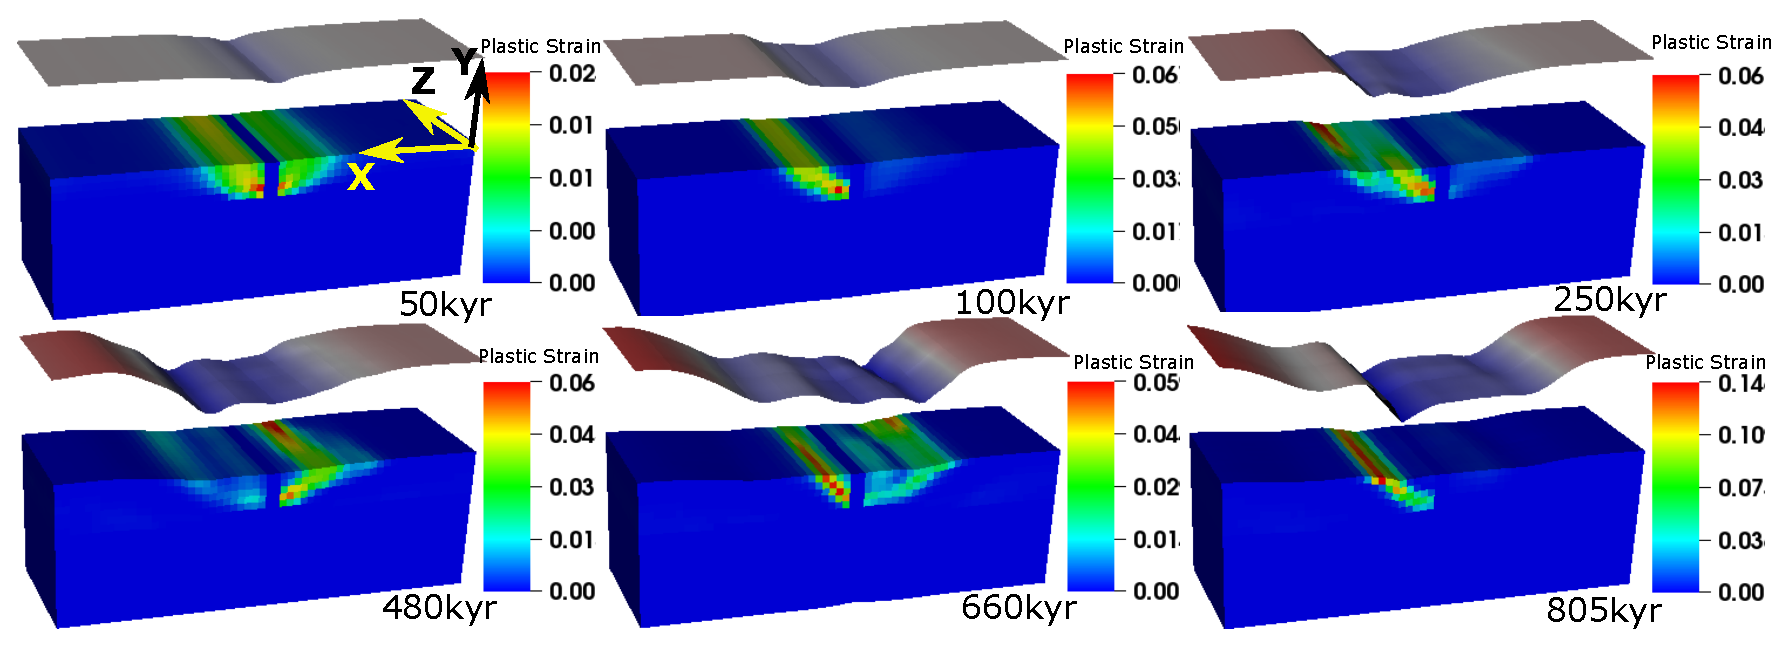
\includegraphics[width=1.0\textwidth]{./Figures/fig_Results1_3.eps}
  \caption{M88ConT2 (Table~\hyperref[Tab1_1]{\ref{Tab1_1}}). Reference model two: constant M$=0.8$ along the ridge-axis (i.e. Z axis). Type two weakening.}
 \label{fig_Results1_3}
\end{figure}   

Another reference model is the model with constant M$=0.8$ along the ridge axis as a comparison to the changing M models.

As shown in Figure~\hyperref[fig_Results1_3]{\ref{fig_Results1_3}}, this constant M along the ridge-axis model creates a median valley of $\sim 20km$ in width and $1\sim2km$ in depth which is similar to generally observation of Mid-Atlantic Ridges. The width and depth of the median valley is almost constant along the ridge-axis. The variation along the ridge-axis in breakaway and termination as well as the existence of corrugation mentioned in reference model one are not observed. 


\subsection{Effects of the functional forms of M variation}
As shown in the \annote[EC]{tables}{which table? Specify.}, \add[EC]{the models with} \annote[EC]{M28}{Before starting to use this notation, define and explain it first!} with Type one weakening is \annote[EC]{the only M range that has three functional forms data points available}{This sentence gives an impression that you didn't want to use these three but had no choice but to. This is not the case, I belive. Probably you'd want to point out that one of these three is the reference model that has been fully described earlier. So, we are in a better position to compare it with similar models with different functional forms. In fact, I think this introductory sentence can be thrown out.} 

\change[EC]{There are two phenomena that show distinct differences with respect to different functional forms.}{By comparing M28LinT1 with M28SinT1 and M28sqrtT1, I identified two main characteristics in the different behaviors of these models due to different functional forms of M variation.} One is the geometry and timing of the secondary fault. The other is the ``Cut back'' behavior. \annote[EC]{mostly observed in the square root model.}{No need to spill the beans.}

\begin{figure}[h]
  \centering
    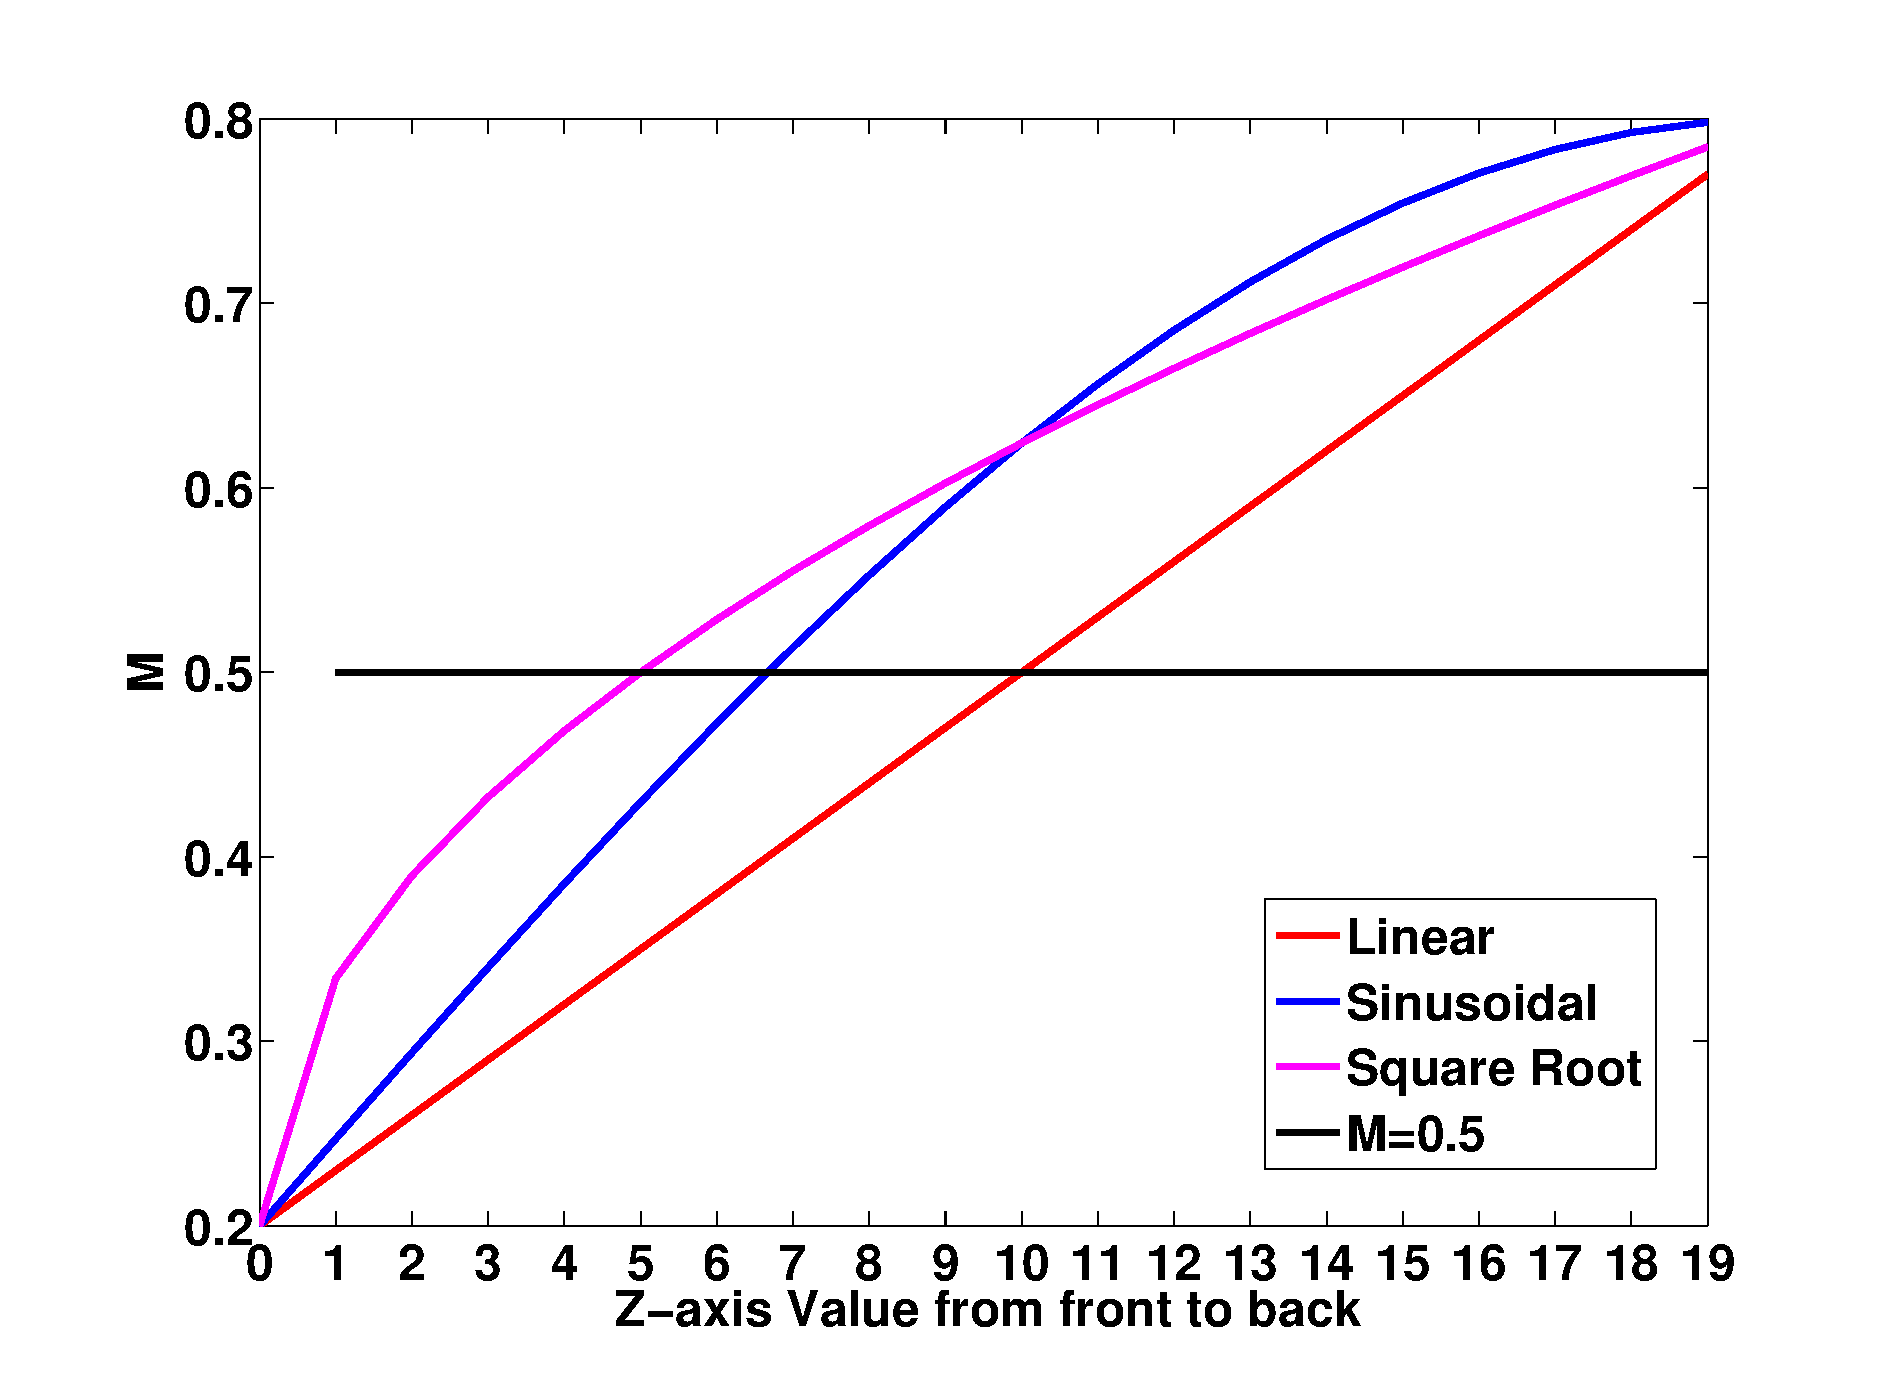
\includegraphics[width=0.6\textwidth]{./Figures/fig_Results3_1.eps}
  \caption{Three functional forms of M variation comparison. They begin to exceed the M$=0.5$ black line at Z=10, 7, 5 for linear, sinusoidal and square root respectively.}
 \label{fig_Results3_1}
\end{figure}   

\paragraph{Second Fault}\label{para_SecondaryFault}

For the linear functional form, the second fault \note[XT]{add a definition of secondary fault in the begining, here add a link of figure about primary and sec fault, enlarge the second fault and add label in the figure and use it here } at the high M side has started accommodating most of the extension at around 900kyrs and the initial detachment becomes inactive \note[XT]{(Figure~\hyperref[fig_Results4_2]{\ref{fig_Results4_2}})}{refer to Figure 8.f is better}. It nucleates from the ridge center where M$=0.5$ and then propagates to the M$=0.8$ end. %(Figure~\hyperref[fig_Results3_1]{\ref{fig_Results3_1}} where the red line begin to exceeds 0.5 at Z$=10$).
 %This secondary fault creates another dome with initial composition likely to be volcanic rather than ultramafic, however, as it evolves, if it can last long enough to cut through the whole crust, mantle materials might exhume to the surface. The composition of the domes observed at Kane magamullions is similar to this mechanism between ultramafic babel dome and eastern to it the crustal inside-corner high.  its spatial distribution is at M$>0.5$ region.

\begin{figure}[h]
  \centering
    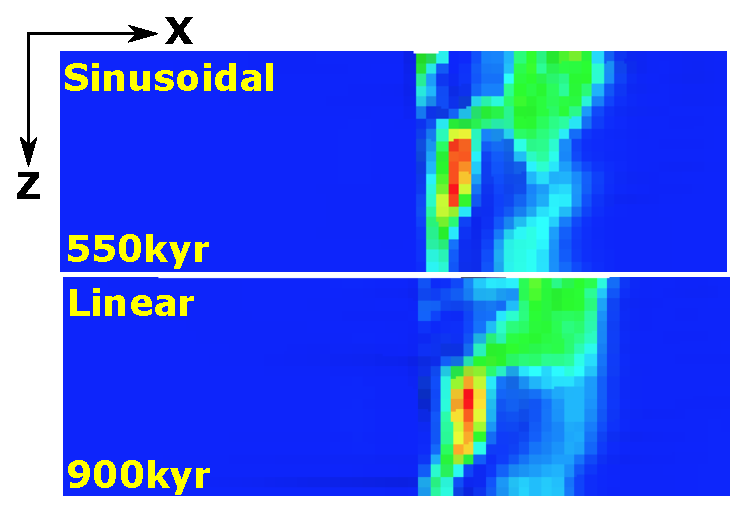
\includegraphics[width=0.6\textwidth]{./Figures/fig_Results4_2_secondary_fault_length_comparison.eps}
  \caption{M28LinT1 versus M28SinT1 (Table~\hyperref[Tab1_1]{\ref{Tab1_1}}). Secondary fault length comparison between linear and sinusoidal. Around 13 elements in length for sinusoidal compared to 11 elements for linear.}
 \label{fig_Results4_2}
\end{figure}   

For the sinusoidal form, the second fault begins to form at a much earlier time around 550kyrs (Figure~\hyperref[fig_Results4_2]{\ref{fig_Results4_2}}). The sinusoidal form consistently has higher M values than the linear form (Fig. 10), implying a greater amount of magma supply. %The total force to push the hanging wall of the detachment away from the dike is greater than that of linear. The larger the force,
The first forming fault moves away from the ridge axis faster and locks earlier in the case of the sinusoidal form. As a result, the second fault appears earlier than in the case of the linear M variation. In addition, the sinusoidal form produces the second fault with a greater along-strike dimension than the linear form because this length is proportional to the length of the M $\ge$ 0.5 portion of the ridge (Figure~\hyperref[fig_Results3_1]{\ref{fig_Results3_1}}). 
For square root, there is no secondary fault forming because the ``cut back'' behavior releases the tensional stress in the hanging wall.

\paragraph{Cut-back}\label{para_CutBack}

\begin{figure}[h]
  \centering
    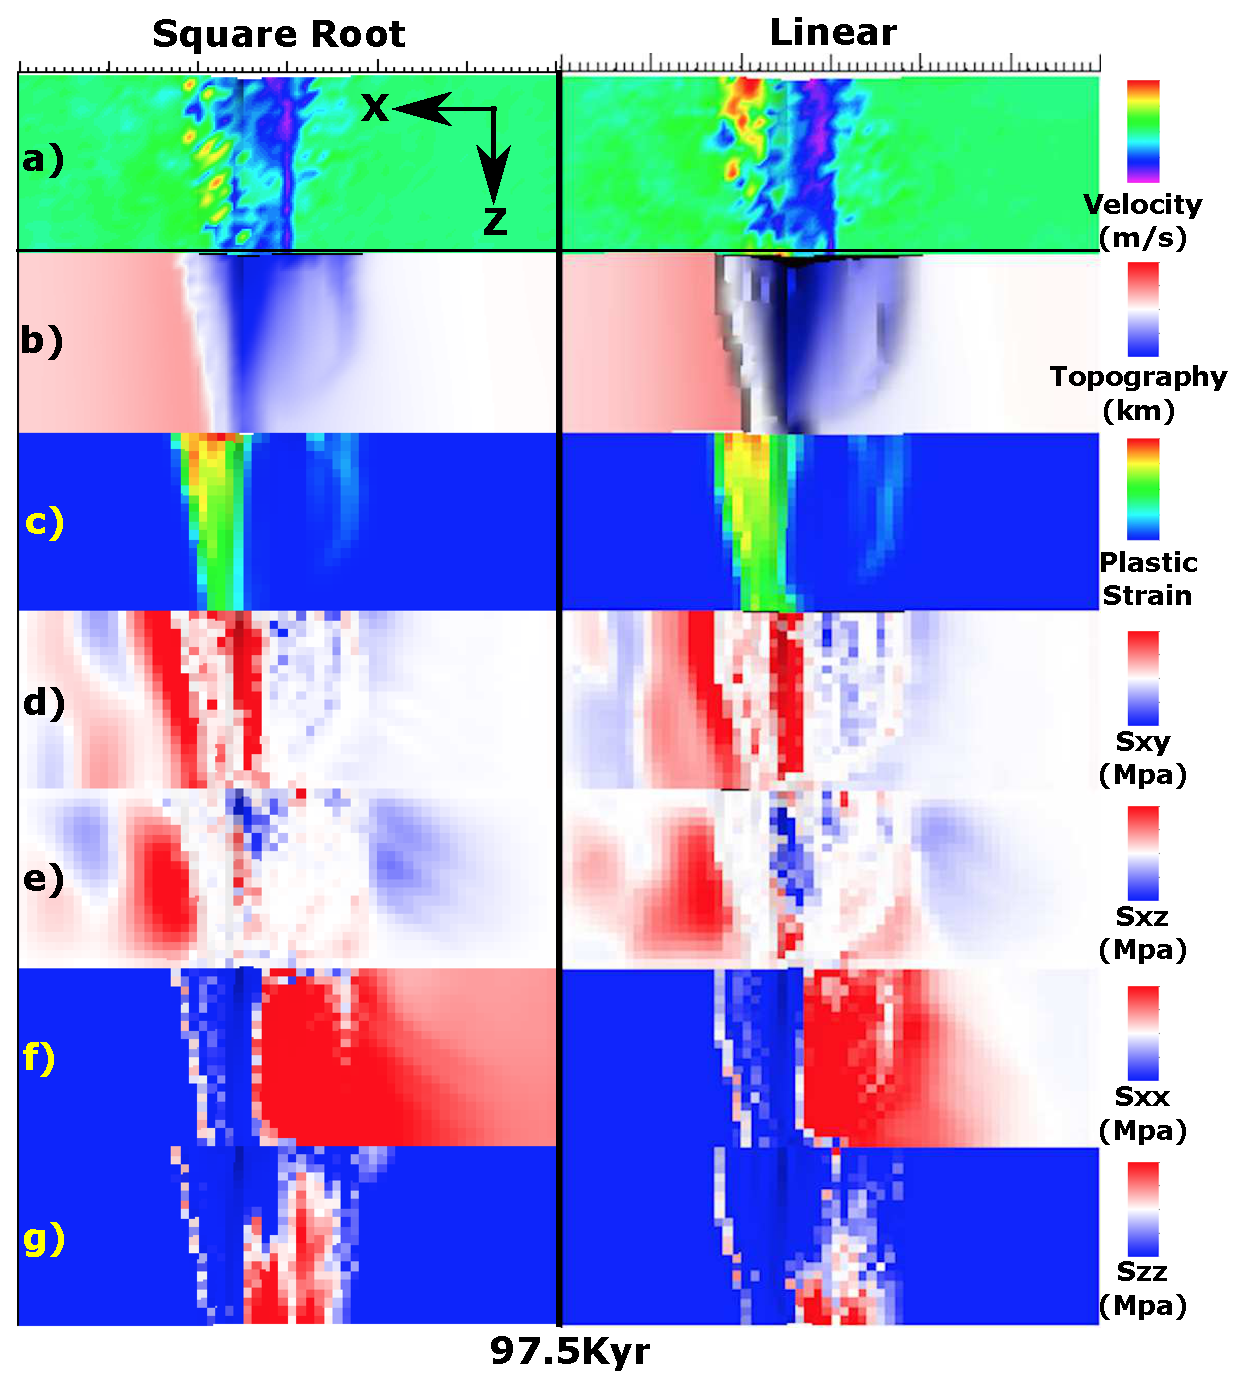
\includegraphics[width=0.6\textwidth]{./Figures/fig_Results4_3_sqrt_vs_lin_cut_back_97kyr.eps}
  \caption{M28LinT1 versus M28SqrtT1 (Table~\hyperref[Tab1_1]{\ref{Tab1_1}}) at 97kyr. View from top of the model.}
 \label{fig_Results4_3_1}
\end{figure}  

\begin{figure}[h]
  \centering
    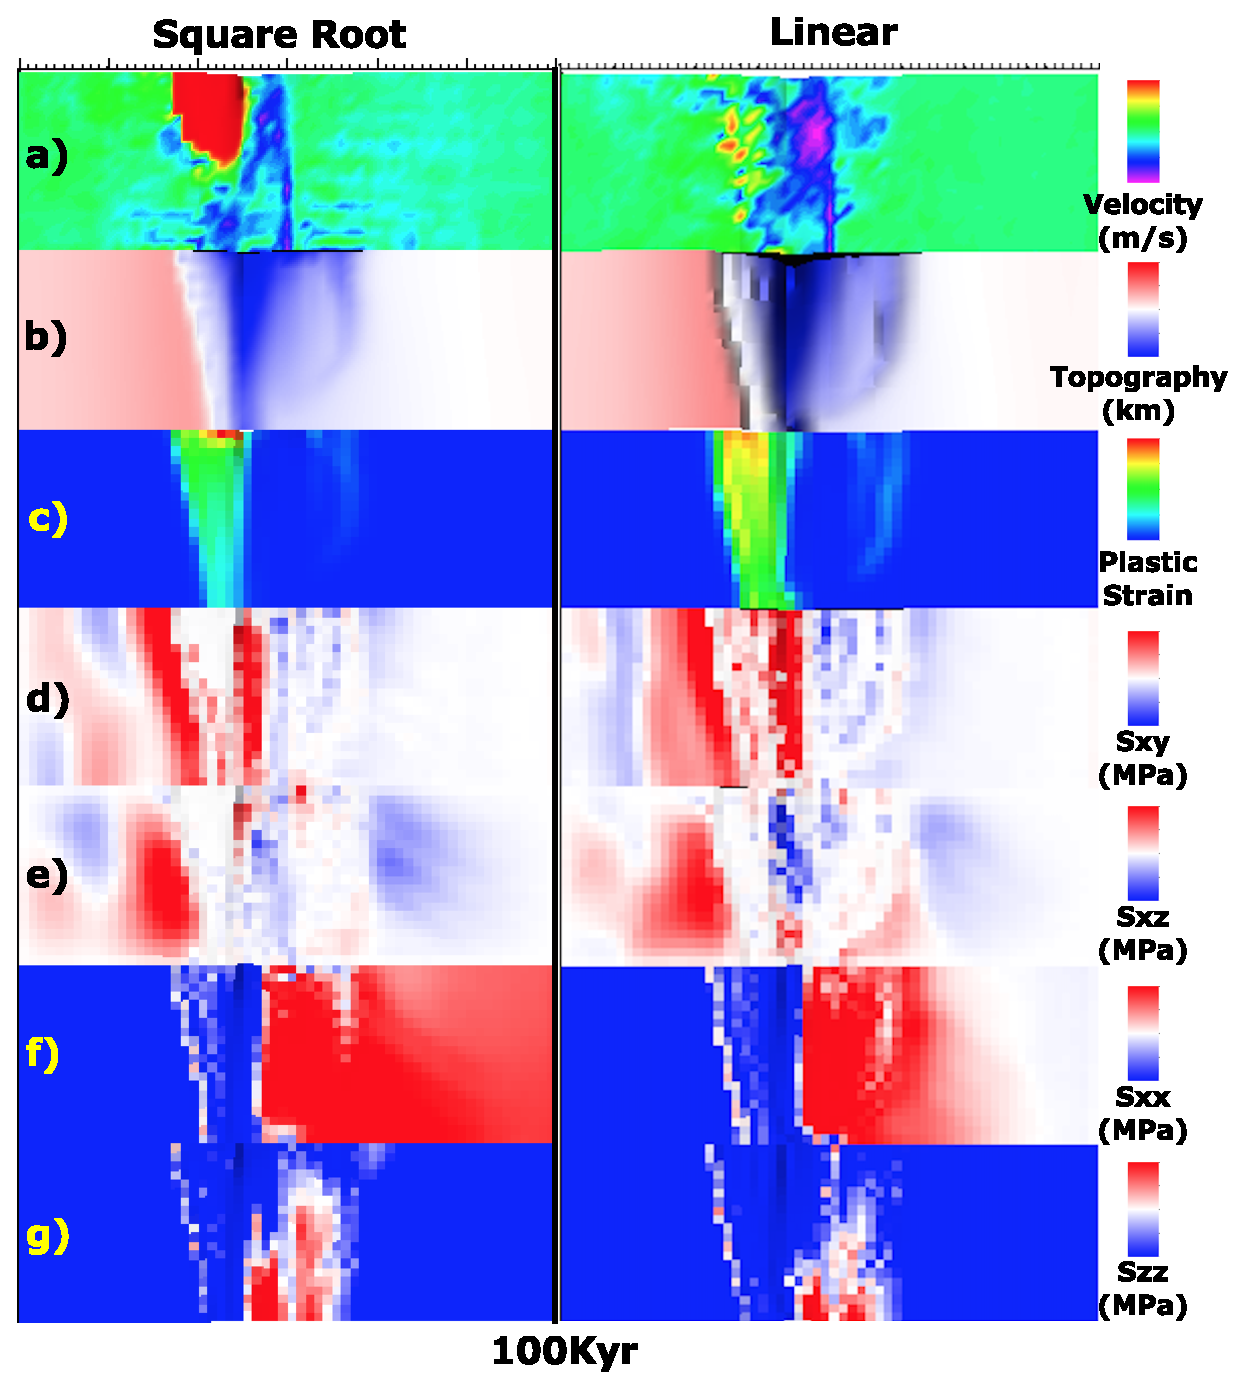
\includegraphics[width=0.6\textwidth]{./Figures/fig_Results4_3_sqrt_vs_lin_cut_back_100kyr.eps}
  \caption{M28LinT1 versus M28SqrtT1 (Table~\hyperref[Tab1_1]{\ref{Tab1_1}}) at 100kyr. View from top of the model.}
 \label{fig_Results4_3_2}
\end{figure} 

\note[XT]{Define a cut-back and think about a different name.}
The cut-back characterizes but are not limited to the models with the square root form of M variation.\note[XT]{exclusively about the square root models?} As shown in Figure~\hyperref[fig_Results4_3_1]{\ref{fig_Results4_3_1}}, Figure~\hyperref[fig_Results4_3_1]{\ref{fig_Results4_3_2}} and Figure~\hyperref[fig_Results4_4]{\ref{fig_Results4_4}} \note[XT]{Bring up Fig. 26 here and incude only the cut-back panel.}, between 97.5kyr and 100kyr, there are cut-backs in the square root model M28SqrtT1 at the low M side where hanging walls with surface area of $\sim$ 60 km$^{2}$ and $\sim$ 120 km$^{2}$ (the red block) suddenly rebound backwards towards the ridge-axis as seen in 100kyr and 160kyr (Figure~\hyperref[fig_Results4_3_1]{\ref{fig_Results4_3_2}.a} and Figure~\hyperref[fig_Results4_4]{\ref{fig_Results4_4}.d,e,f}), along with sudden topography drop (Figure~\hyperref[fig_Results4_4]{\ref{fig_Results4_4}.d,e} 2nd row), $\sigma_{xy}$ and $\sigma_{xz}$ released, termination falls back (Figure~\hyperref[fig_Results4_4]{\ref{fig_Results4_4}.f} 3rd row). 

\subsection{Effects of the weakening rate}

According to our available twelve 3D models, we have three pairs of models that both have Type one and Type two \note[XT]{might want to add a ref to the section defining these.} weakening while the range of M and functional form are maintained to be the same. They are M57SinT1/T2, M58SinT1/T2 and M58SqrtT1/T2.

\paragraph{M57SinT1 versus M57SinT2}

\begin{figure}[h]
 \centering
  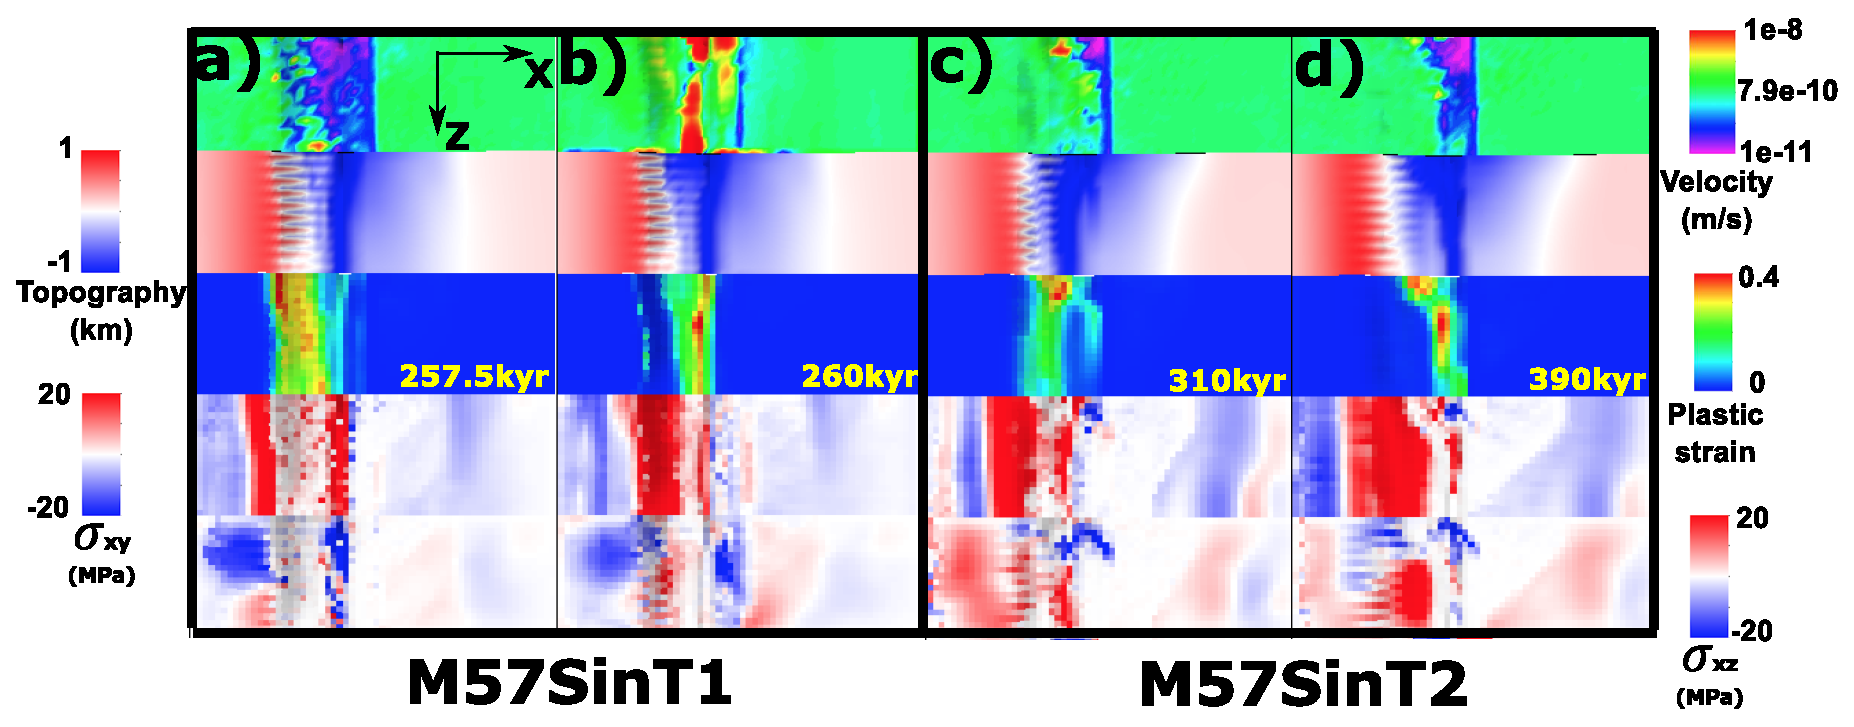
\includegraphics[width=1.0\textwidth]{./Figures/fig_Results_Weakening_2_M57SinT1VST2_CutbackVSsecondaryFault.eps}
 \caption{M57SinT2 versus M57SinT1 (Table~\hyperref[Tab1_1]{\ref{Tab1_1}}). a) and b) are for M57SinT2, c) and d) are for M57SinT1.}
\label{fig_Results_Weakenging_2}
\end{figure}

Initially, both models develop normal faults on both sides of the ridge axis\note[XT]{no hyphen in ``ridge axis''.} at the low M side. In the model with the faster weakening rate (M57SinT1), faults propagate toward the high M side and cut through the whole crust by 25kyr but this process completes later at 50 kyr in the model with the slower weakening rate (M57SinT2). At around 310kyr, the second fault appears at the high M side\note[XT]{instead of z=5, use a M value.} of M57SinT2 while where M $<=$\annote[XT]{5}{some M value}, the initial fault remains active (Figure~\hyperref[fig_Results_Weakenging_2]{\ref{fig_Results_Weakenging_2}.a) and b)}). However, when the weakening is fast (M57SinT1), cut-back happens at around 260kyr and help to maintain a high angle fault with closer to ridge-axis termination. The initial fault remains, no secondary fault forming (Figure~\hyperref[fig_Results_Weakenging_2]{\ref{fig_Results_Weakenging_2}.a) and b)}). In addition, the width of median valley at low M side is wider for M57SinT2 than M57SinT1 (Figure~\hyperref[fig_Results_Weakenging_2]{\ref{fig_Results_Weakenging_2}.a) and b) versus c) and d)}) due to slower weakening (Type two) alows a more distributed tensional stress $\sigma_{xx}$ rather than fast weakening that once a fault is established, larger amount of tensional stress $\sigma_{xx}$ will be released at the fault.  

\begin{figure}[h]
 \centering
  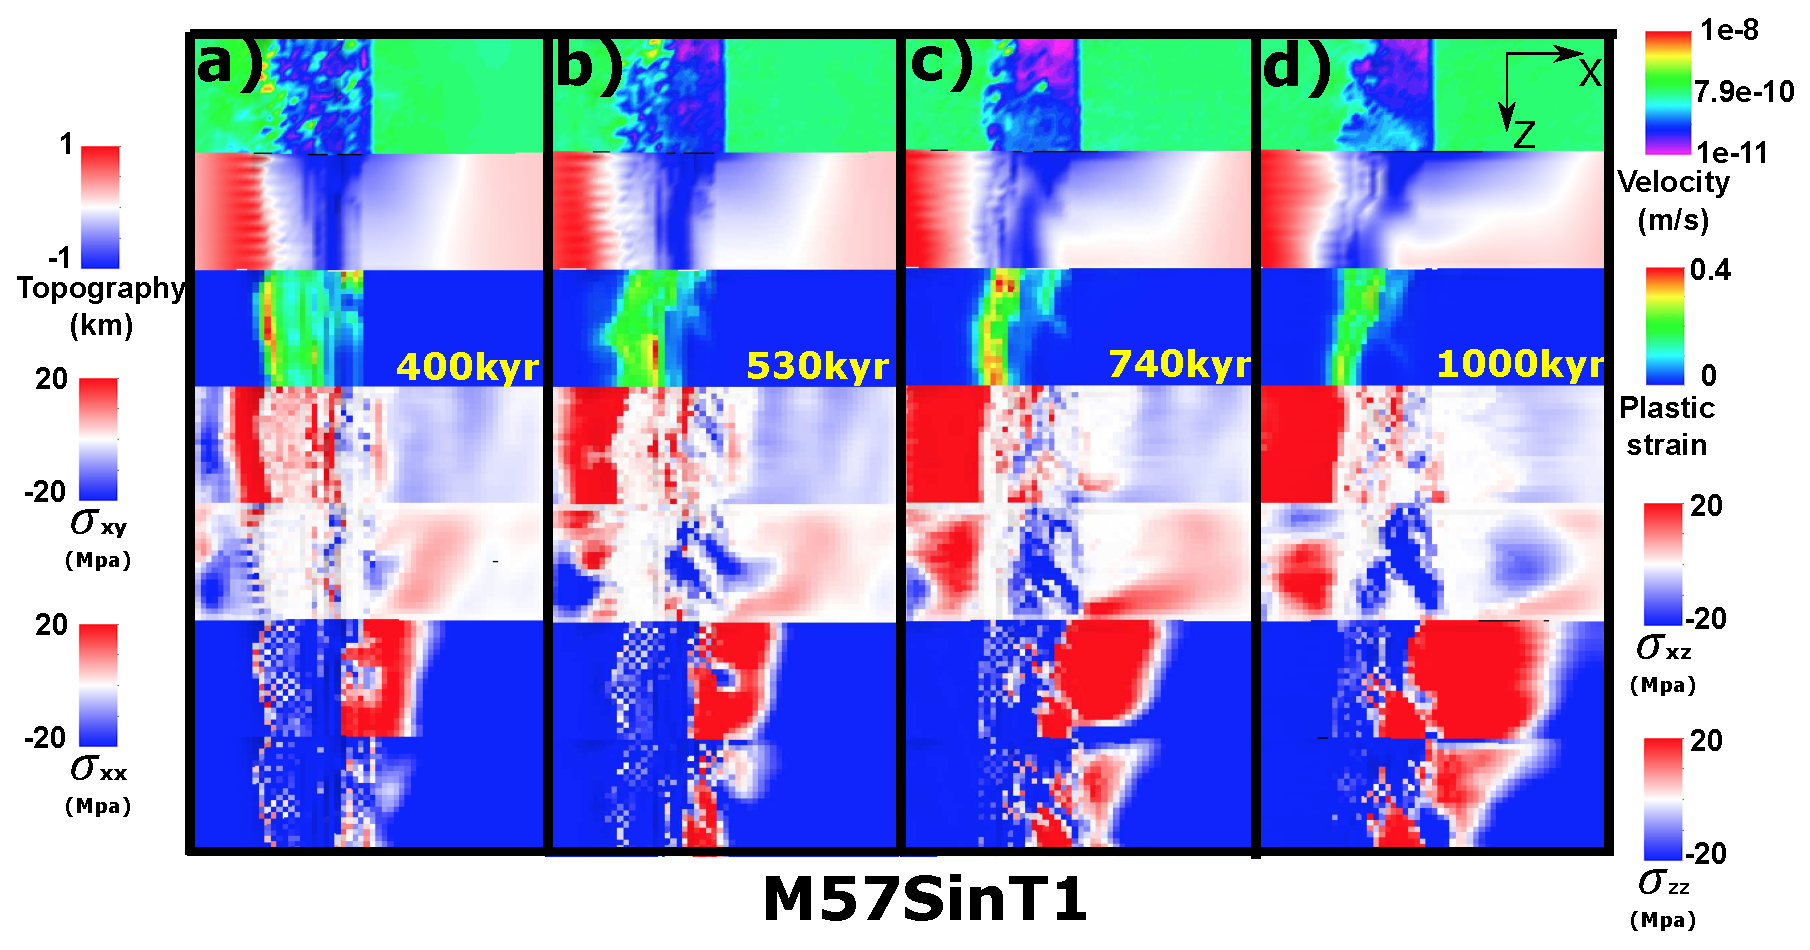
\includegraphics[width=1.0\textwidth]{./Figures/fig_Results_Weakening_3_M57SinT1_time_evolution.eps}
 \caption{M57SinT1 (Table~\hyperref[Tab1_1]{\ref{Tab1_1}}) faulting and stress evolution with respect to time.}
\label{fig_Results_Weakenging_3}
\end{figure}

\paragraph{M57SinT1}\label{para_M57SinT1}

For M57SinT1, as shown in Figure~\hyperref[fig_Results_Weakenging_3]{\ref{fig_Results_Weakenging_3}}, at 400kyr (Figure~\hyperref[fig_Results_Weakenging_3]{\ref{fig_Results_Weakenging_3}.a}), there is a antithetic fault forming at the low M side accommodating part of the extension, which results in a curved termination at the far frontier. As it evolve (530kyr (Figure~\hyperref[fig_Results_Weakenging_3]{\ref{fig_Results_Weakenging_3}.b})), the termination at the low M side further recedes backward while the termination at the center (Z$=11\sim13$) extends further. This curved termination leads to a curved topography (white curve in the second row). As the fault evolves and bends further away from the axis, at the time of 740kyr, another antithetic fault forming again at the low M side (Figure~\hyperref[fig_Results_Weakenging_3]{\ref{fig_Results_Weakenging_3}.c}). It doesn't take the place of initial fault and disapear soon, however, it again releases tensional stress and results in that the termination at far front recedes backward. At 1000kyr (Figure~\hyperref[fig_Results_Weakenging_3]{\ref{fig_Results_Weakenging_3}.d}), an Atlantiss Massif shape OCC is produced (low M side (lower magma supply) has a wider dome and high M side (higher magma supply) has a narrower dome) due to the along ridge-axis termination evolution. Corrugations with wavelength varying from hundreds to kilometers are also created.       

\begin{figure}[h]
 \centering
  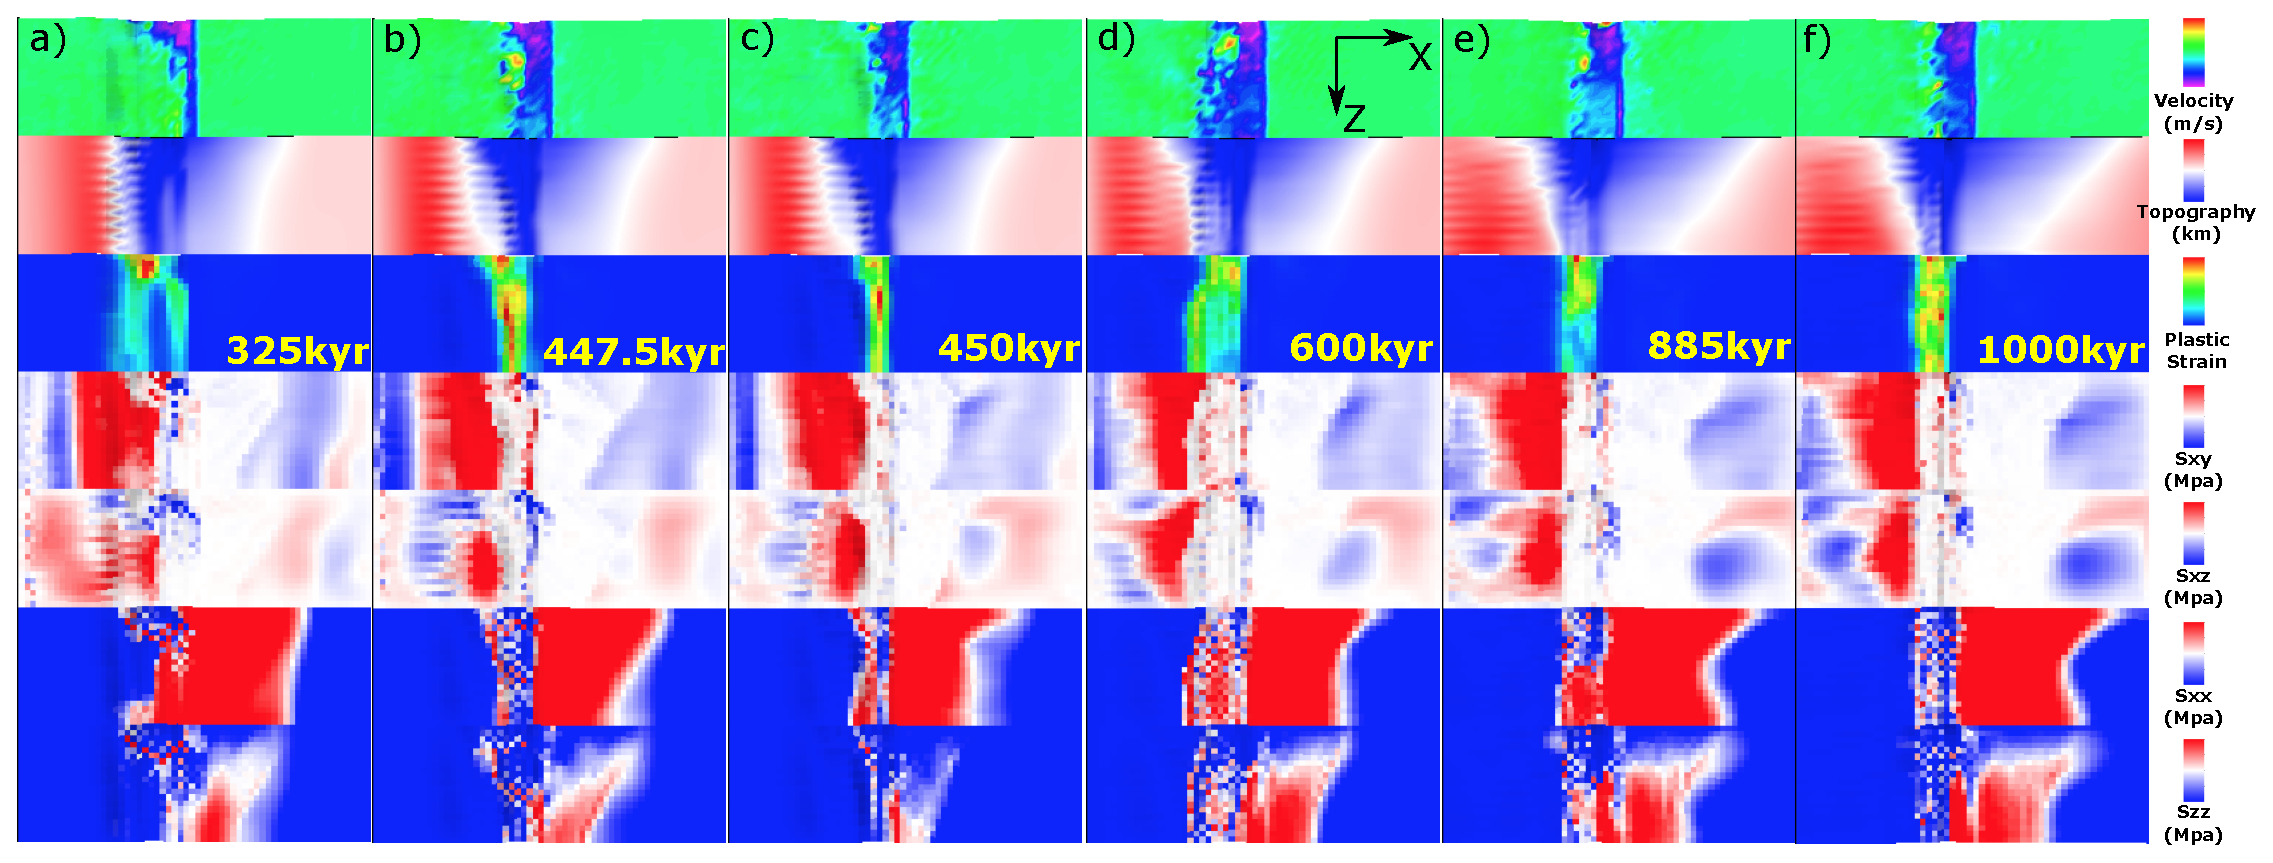
\includegraphics[width=1.0\textwidth]{./Figures/fig_Results_Weakening_4_M57SinT2_time_evolution.eps}
 \caption{M57SinT2 (Table~\hyperref[Tab1_1]{\ref{Tab1_1}}) faulting and stress evolution with respect to time.}
\label{fig_Results_Weakenging_4}
\end{figure}

\paragraph{M57SinT2}\label{para_M57SinT2}

For M57SinT2, as shown in Figure~\hyperref[fig_Results_Weakenging_4]{\ref{fig_Results_Weakenging_4}}, instead of maintaining one fault all the time for M57SinT1, it creats secondary fault at high M side with different mechanism several times. A secondary fault is created at 325kyr (Figure~\hyperref[fig_Results_Weakenging_4]{\ref{fig_Results_Weakenging_4}.a}), when a new near axis normal fault take the place of the initial one at high M side. Between 447.5kyr (Figure~\hyperref[fig_Results_Weakenging_4]{\ref{fig_Results_Weakenging_4}.b}) and 450kyr (Figure~\hyperref[fig_Results_Weakenging_4]{\ref{fig_Results_Weakenging_4}.c}), termination falls back, and as it evolve, termination at the high M side extends further at 600kyr (Figure~\hyperref[fig_Results_Weakenging_4]{\ref{fig_Results_Weakenging_4}.d}). At 885kyr (Figure~\hyperref[fig_Results_Weakenging_4]{\ref{fig_Results_Weakenging_4}.e}), a secondary fault propagates from low Z to high Z and terminates the further extended fault at high Z and maintain a near ridge-axis termination.

\subsubsection{M58SinT1 versus M58SinT2}

A major difference between M58SinT1 and M58SinT2 is that M58SinT1 keep faulting at one side of the ridge-axis while M58SinT2's fault alternates.

\begin{figure}[h]
 \centering
  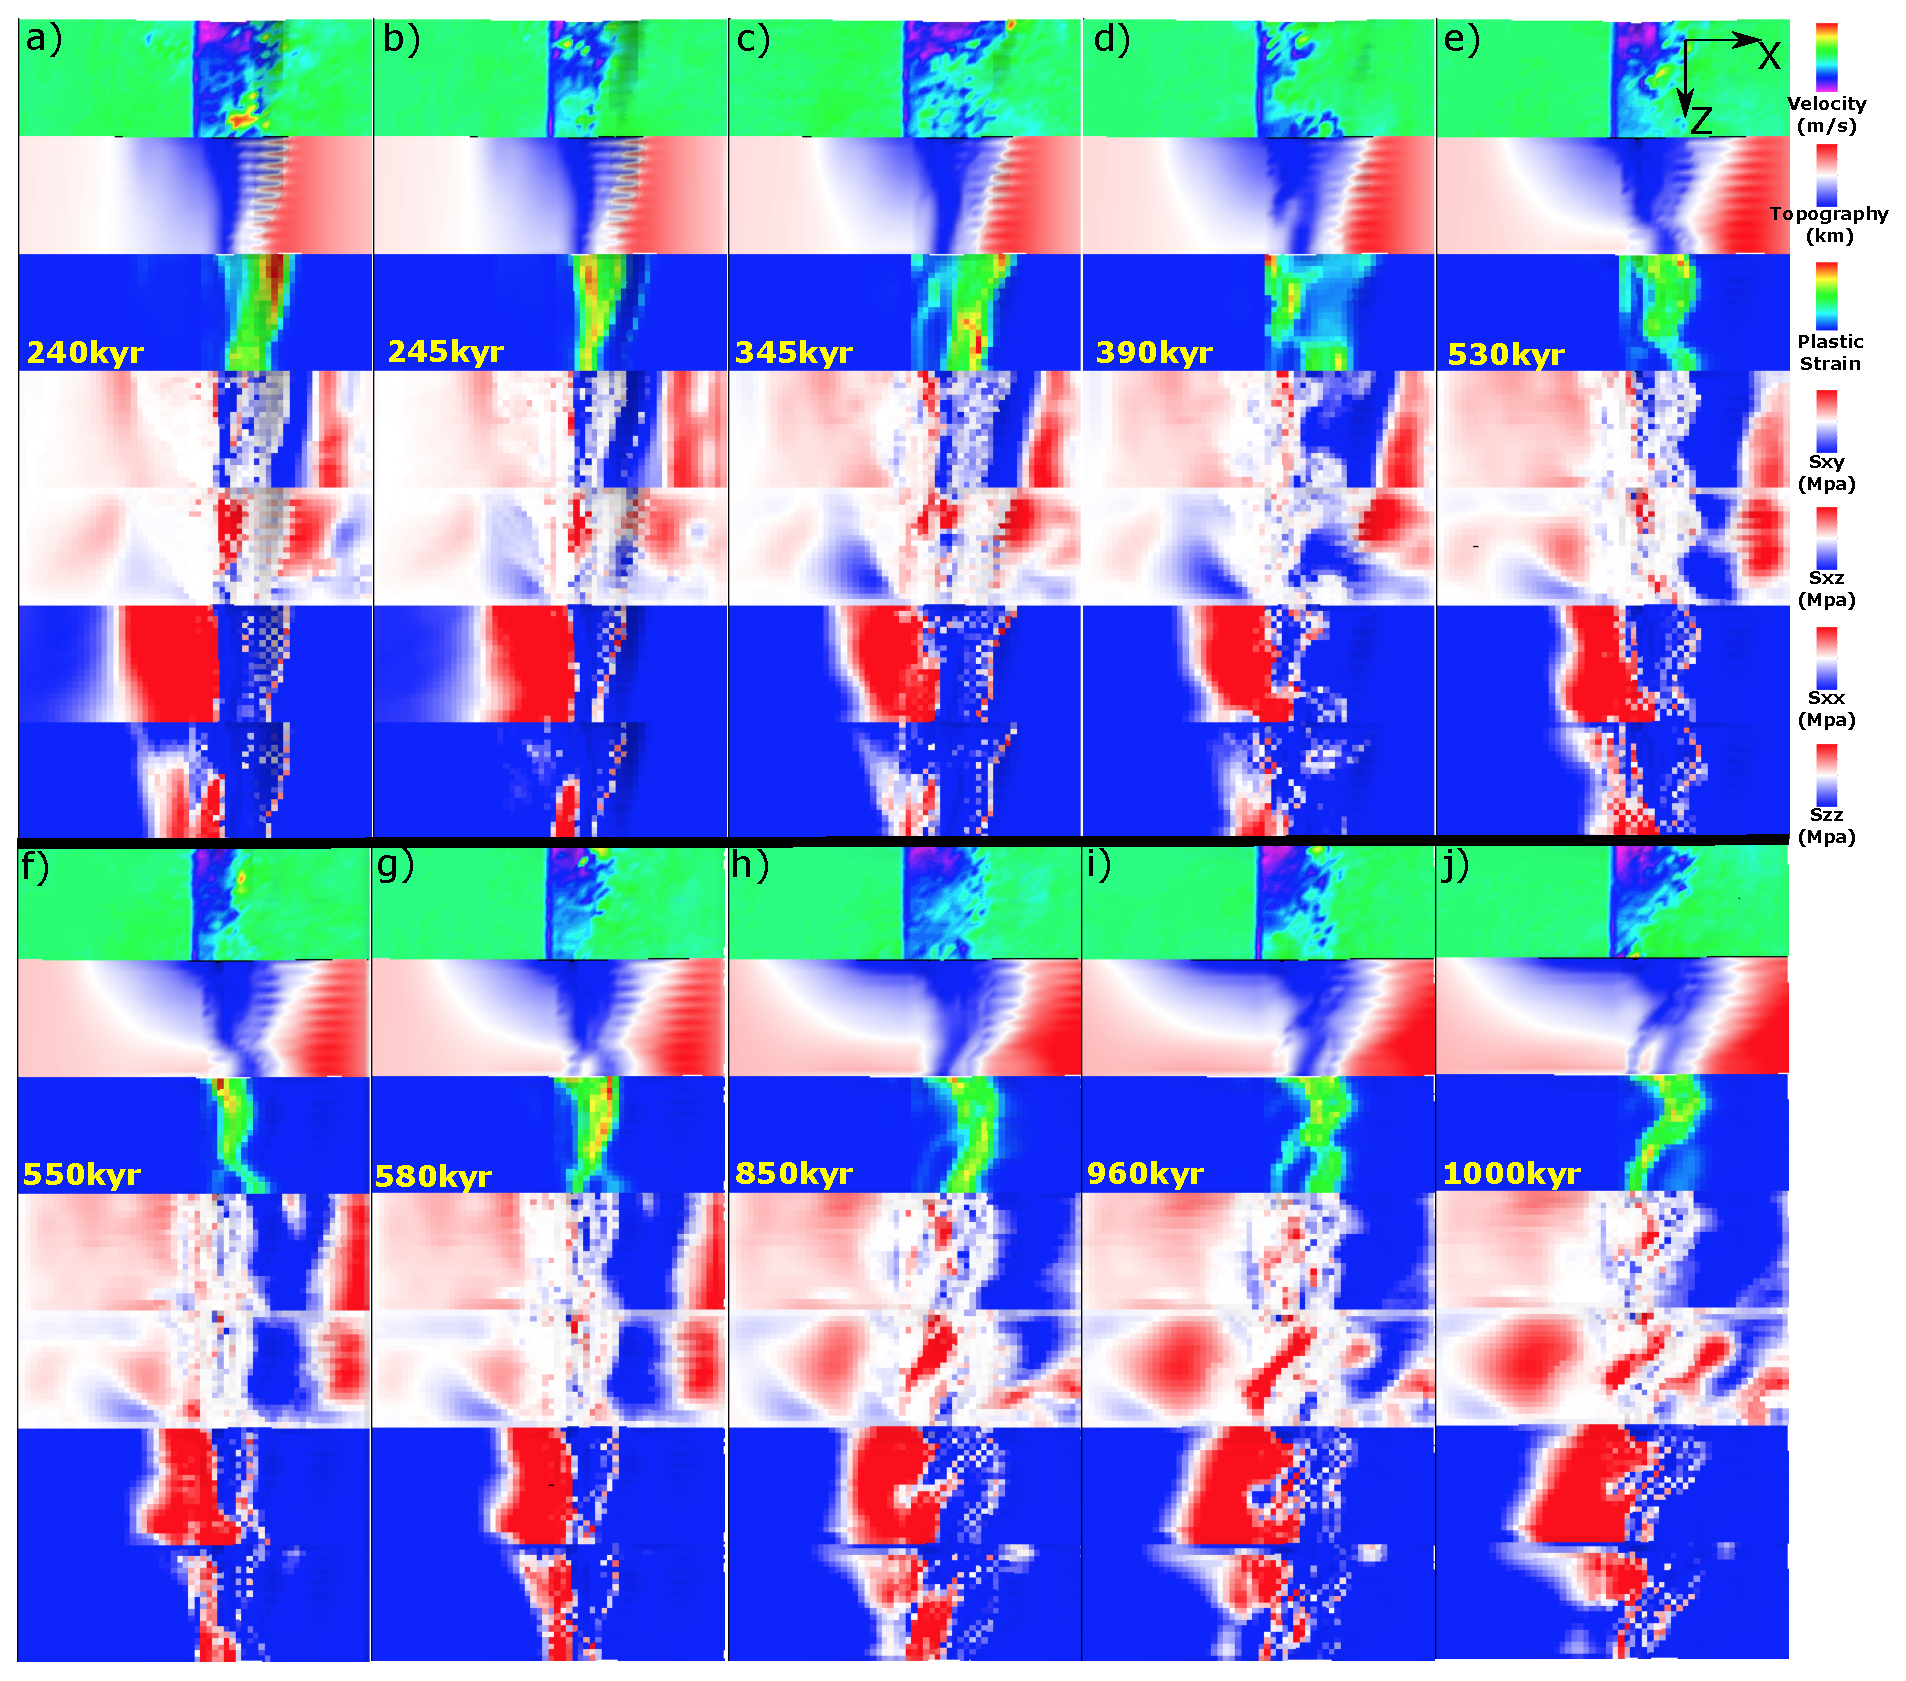
\includegraphics[width=1.0\textwidth]{./Figures/fig_Results_Weakening_5_M58SinT1_time_evolution.eps}
 \caption{M58SinT1 (Table~\hyperref[Tab1_1]{\ref{Tab1_1}}) faulting and stress evolution with respect to time.}
\label{fig_Results_Weakenging_5}
\end{figure}

\paragraph{M58SinT1}\label{para_M58SinT1}

As shown in Figure~\hyperref[fig_Results_Weakenging_5]{\ref{fig_Results_Weakenging_5}}, in 1Myr, the fault keeps on the right hand side of the ridge-axis. It evolves dynamically. Between 240kyr (Figure~\hyperref[fig_Results_Weakenging_5]{\ref{fig_Results_Weakenging_5}.a}) and 245kyr (Figure~\hyperref[fig_Results_Weakenging_5]{\ref{fig_Results_Weakenging_5}.b}), there is a cut back. At 345kyr (Figure~\hyperref[fig_Results_Weakenging_5]{\ref{fig_Results_Weakenging_5}.c}), at low Z side, there are two offsetted antithetic faults (Z=$1\sim2$ and Z=$5\sim9$) in the hanging wall begin to evolve and soon connect to each other forming anastomosing fault zone. At 390kyr (Figure~\hyperref[fig_Results_Weakenging_5]{\ref{fig_Results_Weakenging_5}.d}), the new near axis anastomosing fault zone replace the old further away from ridge-axis detachment. There is dextral $\sigma_{xz}$ forming on the right hand side of the new anastomosing fault zone ((Figure~\hyperref[fig_Results_Weakenging_5]{\ref{fig_Results_Weakenging_5}.d}), row 5) due to the offset between the new near axis fault at low Z side and extended further fault at high Z side and leads to the development of a $\sim45\degree$ shear zone connection between the new near axis fault zone at low Z side and the further away from axis original detachment at high Z side. It also creates a curved termination which will lead to a curved topography (boundary between blue and white) seen at 530kyr (Figure~\hyperref[fig_Results_Weakenging_5]{\ref{fig_Results_Weakenging_5}.e}). Note that this curved termination can be a mechanism for producing large wavelength (several kilometers) undulating corrugations. Between 530kyr (Figure~\hyperref[fig_Results_Weakenging_5]{\ref{fig_Results_Weakenging_5}.e}) and 550kyr (Figure~\hyperref[fig_Results_Weakenging_5]{\ref{fig_Results_Weakenging_5}.f}), there is another cut back happens. Terminations fall backwards to near ridge-axis position. At 580kyr (Figure~\hyperref[fig_Results_Weakenging_5]{\ref{fig_Results_Weakenging_5}.g}), at the high Z side, a new near rigde-axis high angle normal fault begin to initiate under the assistance of rotational force from low Z side due to along ridge-axis coupling. This produces a large rider block with several kilometers in its length scale. Previous ``S'' curved termination now evolves to a half circle curve and it soon affects the curve of topography as seen at 850kyr (Figure~\hyperref[fig_Results_Weakenging_5]{\ref{fig_Results_Weakenging_5}.h}). Due to along ridge-axis variation in diking, a large sinistral shear zone (red region $\sim40\degree$ oblique to ridge axis seen in 5th row of 960kyr (Figure~\hyperref[fig_Results_Weakenging_5]{\ref{fig_Results_Weakenging_5}.i})) keep developing and cut the circle curved fault zone at 850kyr (Figure~\hyperref[fig_Results_Weakenging_5]{\ref{fig_Results_Weakenging_5}.h}) into a new fault zone with higher curvature as seen in 1000kyr (Figure~\hyperref[fig_Results_Weakenging_5]{\ref{fig_Results_Weakenging_5}.j}).         

\begin{figure}[h]
 \centering
  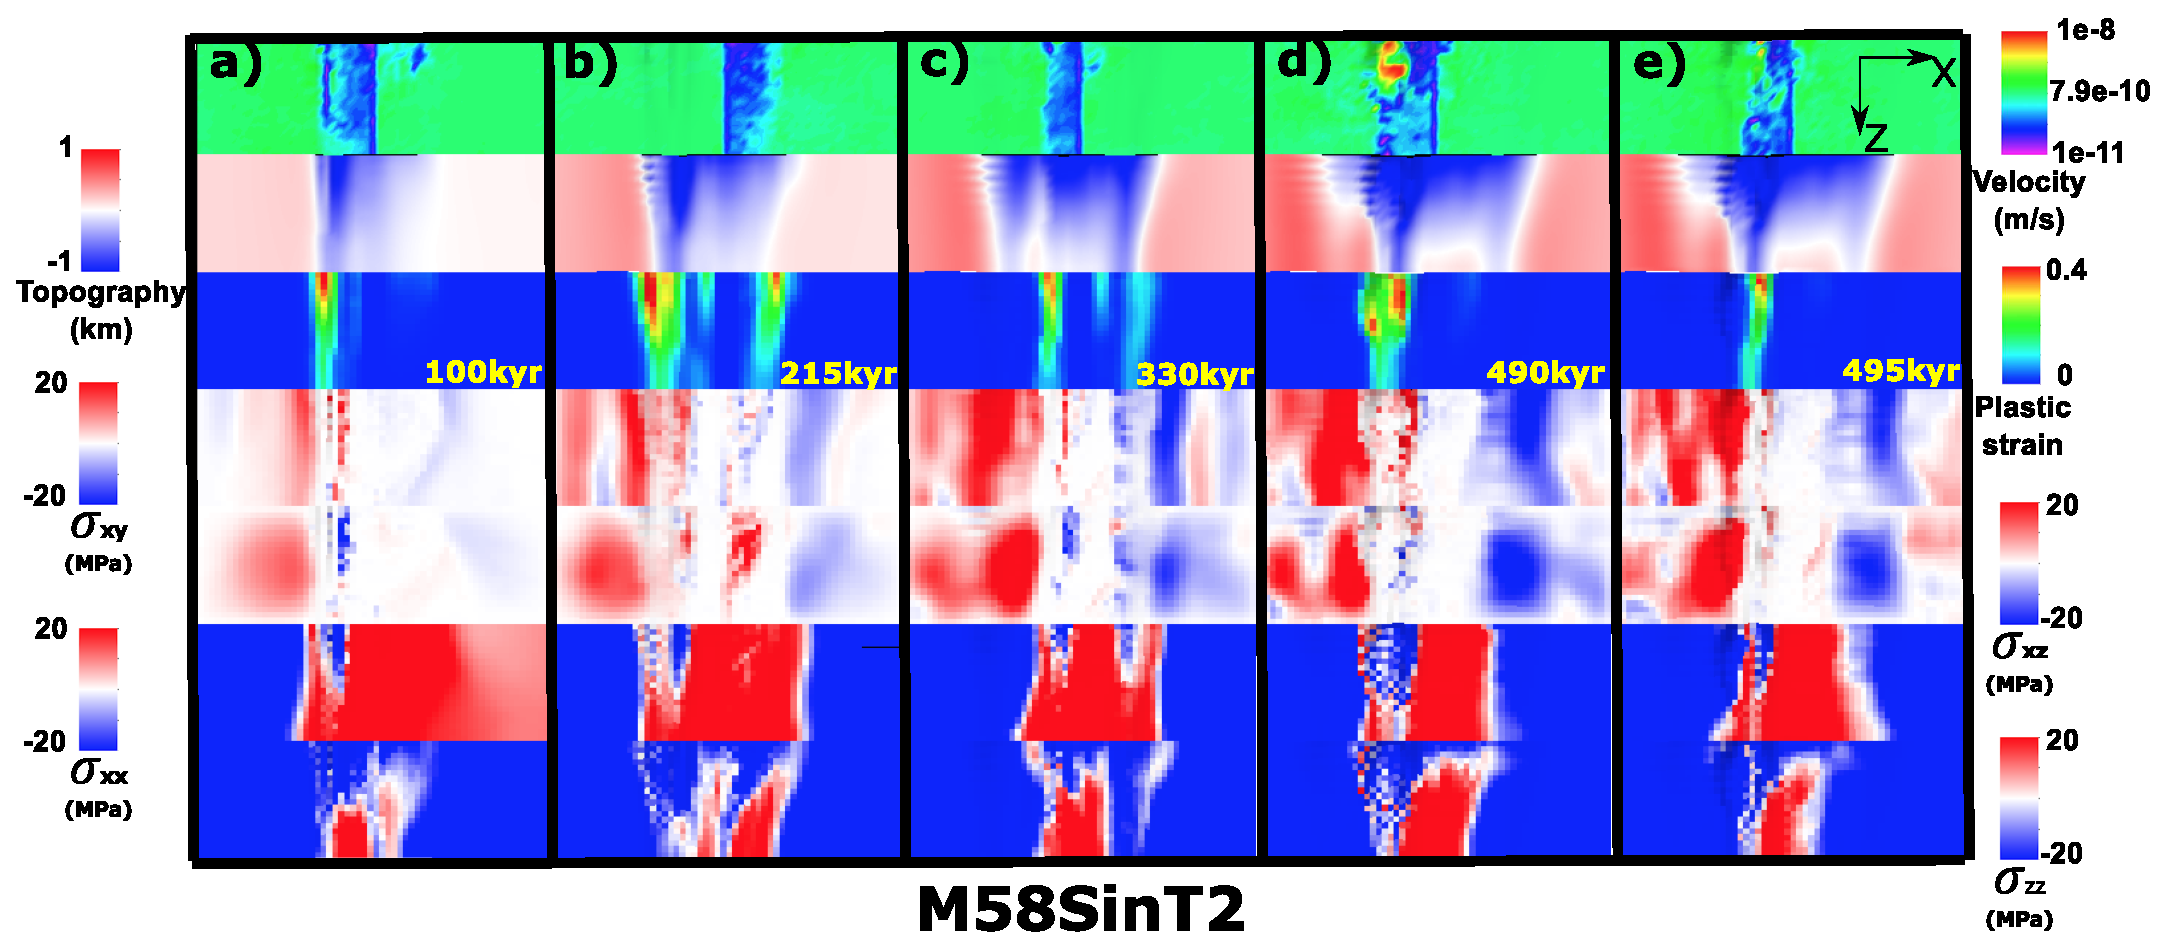
\includegraphics[width=1.0\textwidth]{./Figures/fig_Results_Weakening_6_M58SinT2_time_evolution.eps}
 \caption{M58SinT2 (Table~\hyperref[Tab1_1]{\ref{Tab1_1}}) faulting and stress evolution with respect to time.}
\label{fig_Results_Weakenging_6}
\end{figure}

\paragraph{M58SinT2}\label{para_M58SinT2}

As shown in Figure~\hyperref[fig_Results_Weakenging_6]{\ref{fig_Results_Weakenging_6}}, the fault initiates on the left hand side of the ridge-axis (Figure~\hyperref[fig_Results_Weakenging_6]{\ref{fig_Results_Weakenging_6}.a}). Low Z side extends further than high Z side. It takes around 100kyr to form into a localized fault plane due to slower rate of weakening. At 215kyr (Figure~\hyperref[fig_Results_Weakenging_6]{\ref{fig_Results_Weakenging_6}.b}), another fault on the conjugate plate begin to evolve and replaces the initial one. As seen from (Figure~\hyperref[fig_Results_Weakenging_6]{\ref{fig_Results_Weakenging_6}.b}), corrugations are created at low Z side. At 330kyr, a third fault forming at the left hand side of the ridge-axis. Between 490kyr (Figure~\hyperref[fig_Results_Weakenging_6]{\ref{fig_Results_Weakenging_6}.d}) and 495kyr (Figure~\hyperref[fig_Results_Weakenging_6]{\ref{fig_Results_Weakenging_6}.e}), there is a cut back.

\subsubsection{M58SqrtT1 versus M58SqrtT2}
The major difference between M58SqrtT1 and M58SqrtT2 is also whether the normal fault alternates or not.

\paragraph{M58SqrtT1}\label{para_M58SqrtT1}

As shown in Figure~\hyperref[fig_Results_Weakenging_7]{\ref{fig_Results_Weakenging_7}}, initially, there is a 5 element offset between breakaways along the ridge-axis due to along ridge-axis variation in diking (Figure~\hyperref[fig_Results_Weakenging_7]{\ref{fig_Results_Weakenging_7}.a}). At 370kyr (Figure~\hyperref[fig_Results_Weakenging_7]{\ref{fig_Results_Weakenging_7}.b}), there is a vertical tensile failure at Z$=1\sim2$. Two parallel dextral (blue) shear regions are seen (5th row). The low Z shear zone assists in the shear failure observed at 400kyr (Figure~\hyperref[fig_Results_Weakenging_7]{\ref{fig_Results_Weakenging_7}.c}), and it develops into near ridge-axis normal fault (Z=$4\sim12$) and propagates to high Z side which eventually cuts through and reaches Z$=20$ and replaces the initial extended fault at high Z side at 460kyr (Figure~\hyperref[fig_Results_Weakenging_7]{\ref{fig_Results_Weakenging_7}.d}). The vertical tensile failure zone at Z$=1\sim3$ (Figure~\hyperref[fig_Results_Weakenging_7]{\ref{fig_Results_Weakenging_7}.d} 3rd row) begin to evolve and assists in the initiation of a new near ridge-axis high angle normal fault which connect with the fault at the high Z side (Figure~\hyperref[fig_Results_Weakenging_7]{\ref{fig_Results_Weakenging_7}.e}) at 590kyr. At 660kyr (Figure~\hyperref[fig_Results_Weakenging_7]{\ref{fig_Results_Weakenging_7}.f} 3rd row), there is a hint of high angle normal faulting at Z$=1\sim3$ of conjugate plate. But it doesn't develop. At 730kyr (Figure~\hyperref[fig_Results_Weakenging_7]{\ref{fig_Results_Weakenging_7}.g} 5th row), a dextral (blue) shear zone at the low Z side help to create the faulting pattern seen at 780kyr (Figure~\hyperref[fig_Results_Weakenging_7]{\ref{fig_Results_Weakenging_7}.h} 3rd row), a concave termination with a wavelenth of 10 kilometers and it has the potential to create a large wavelength corrugation. Meanwhile, at the low Z side, near the ridge-axis, there is a antithetic fault forming at the hanging wall of the detachment and it later propagates to high Z side (Figure~\hyperref[fig_Results_Weakenging_7]{\ref{fig_Results_Weakenging_7}.i}). From 820kyr to 880kyr, the antithetic fault evolves to near ridge-axis normal fault and connects with the detachment at the high Z side (Figure~\hyperref[fig_Results_Weakenging_7]{\ref{fig_Results_Weakenging_7}.j}). In addition, a tensile failure shows its hint at the low Z side (Z$=1\sim5$) of the conjugate plate.         

\begin{figure}[h]
 \centering
  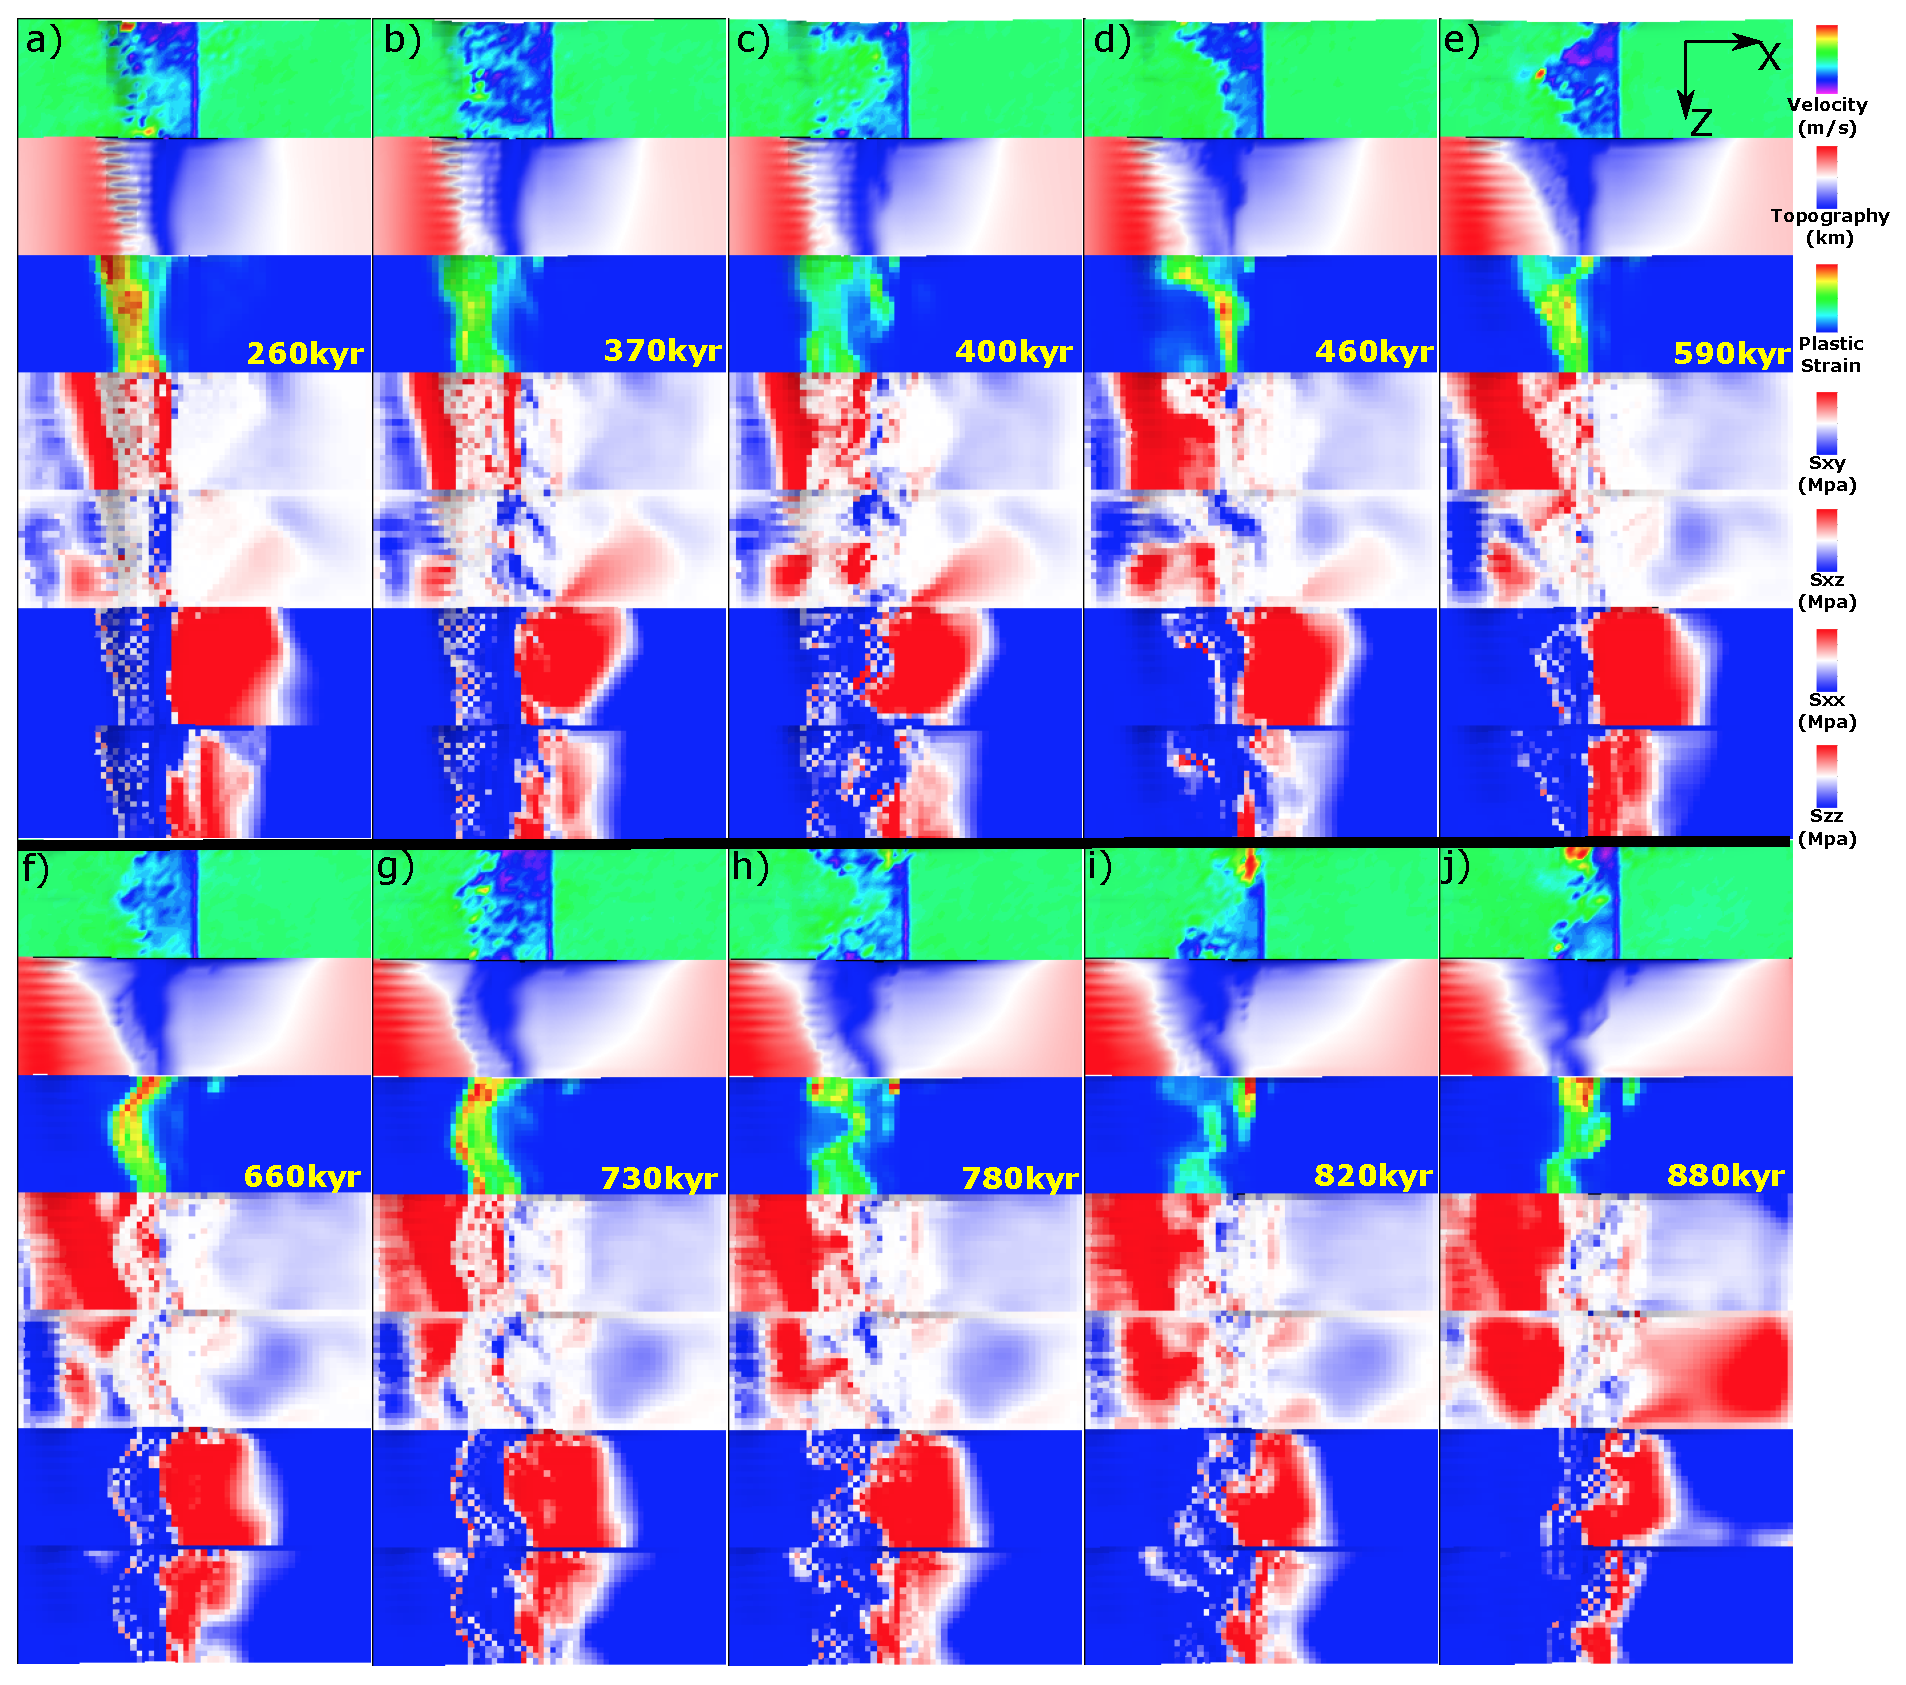
\includegraphics[width=1.0\textwidth]{./Figures/fig_Results_Weakening_7_M58SqrtT1_time_evolution.eps}
 \caption{M58SqrtT1 (Table~\hyperref[Tab1_1]{\ref{Tab1_1}}) faulting and stress evolution with respect to time.}
\label{fig_Results_Weakenging_7}
\end{figure}

\paragraph{M58SqrtT2} \label{para_M58SqrtT2}

\begin{figure}[h]
 \centering
  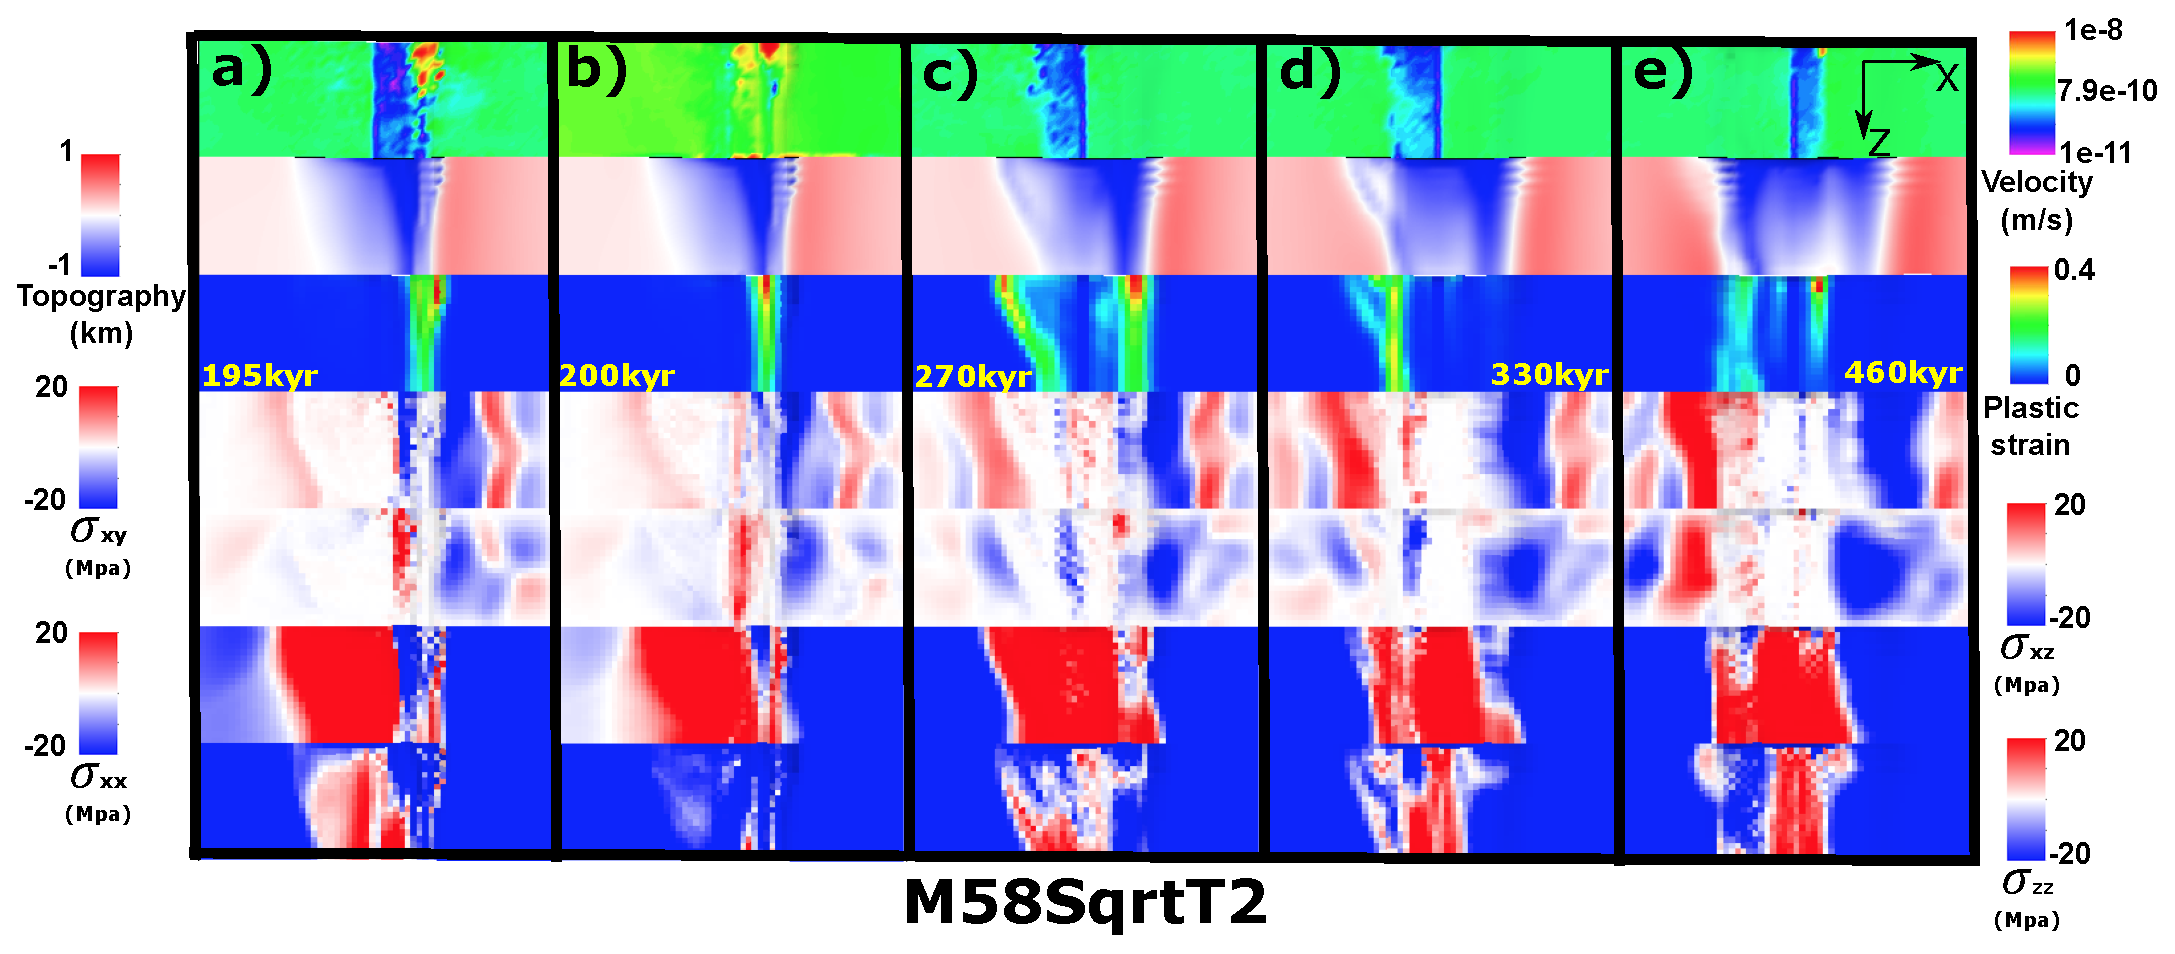
\includegraphics[width=1.0\textwidth]{./Figures/fig_Results_Weakening_8_M58SqrtT2_time_evolution.eps}
 \caption{M58SqrtT2 (Table~\hyperref[Tab1_1]{\ref{Tab1_1}}) faulting and stress evolution with respect to time.}
\label{fig_Results_Weakenging_8}
\end{figure}

As shown in Figure~\hyperref[fig_Results_Weakenging_8]{\ref{fig_Results_Weakenging_8}}, at 195kyr (Figure~\hyperref[fig_Results_Weakenging_8]{\ref{fig_Results_Weakenging_8}.a}), due to transtensional stress at low Z side (Z$=1\sim6$), several corrugations begin to evolve. At conjugate plate, dipping toward axis shear zone $\sigma_{xy}$ (red at 4th row) show its curve and keeps accumulating. $\sigma_{xx}$ is also accummulating on the conjugate plate. Between 195kyr (Figure~\hyperref[fig_Results_Weakenging_8]{\ref{fig_Results_Weakenging_8}.a}) and 200kyr (Figure~\hyperref[fig_Results_Weakenging_8]{\ref{fig_Results_Weakenging_8}.b}), there is a cut back. At 270kyr (Figure~\hyperref[fig_Results_Weakenging_8]{\ref{fig_Results_Weakenging_8}.c}), immediately above and following the curved shape shear $\sigma_{xy}$ zone on the left hand side of the ridge-axis, a new fault begin to evolve and replace the initial fault on the right. At 330kyr (Figure~\hyperref[fig_Results_Weakenging_8]{\ref{fig_Results_Weakenging_8}.d}), at the low Z side, a new near axis high angle normal fault take the place of initial further away from ridge-axis fault partly due to rotational force from along ridge coupling. At 460kyr (Figure~\hyperref[fig_Results_Weakenging_8]{\ref{fig_Results_Weakenging_8}.e}), another normal fault begin to evolve on the right hand side of the ridge-axis.

\subsection{Effects of the range of M variation}
So far, we have three ranges for M variations along the ridge-axis (M28, M57 and M58) with same segment length of 20km. Among the 12 available models, two M58 models and the constant M$=0.8$ model with Type two weakening produce fault alternation while others do not. Generally, M57 and M58 models create a median valley much narrower and shallower than that of M28 models. $\frac{dM}{dz}$ is larger for M28 than M58 and M57.

\subsubsection{M28SinT1 versus M57SinT1 versus M58SinT1}

\paragraph{M57SinT1 versus M58SinT1}\label{M57SinT1 versus M58SinT1}

For description of M57SinT1 evolution with respect to time, please refer to Section~\hyperref[para_M57SinT1]{\ref{para_M57SinT1}} and Figure~\hyperref[fig_Results_Weakenging_3]{\ref{fig_Results_Weakenging_3}}. For description of M58SinT1 evolution with respect to time, please refer to  Section~\hyperref[para_M58SinT1]{\ref{para_M58SinT1}} and Figure~\hyperref[fig_Results_Weakenging_5]{\ref{fig_Results_Weakenging_5}}. Comparing M57SinT1 and M58SinT1, the major difference is that the faulting pattern evolution for M58SinT1 is much more dynamic with a higher frequency of secondary faults, cut back and offseted fault segments connection. For M58SinT1, the new secondary near ridge-axis normal or antithetic faults usually replace the existed one. However, for M57SinT1, diking is not strong enough to create big enough stress perturbation along the ridge-axis for secondary or antithetic faults to take the place of the original one. At the low Z side, near ridge-axis antithetic fault only helps to accommodate tensional stress which help maintain a high angle normal fault with near to ridge-axis termination while the termination at the high Z side gradually move off axis. This creates a OCC with larger dome at lower magma supply side than that of higher magma supply side which is opposite to the shape of OCC created by M58SinT1. 

\paragraph{M28SinT1}\label{para_M28SinT1}

\begin{figure}[h]
 \centering
  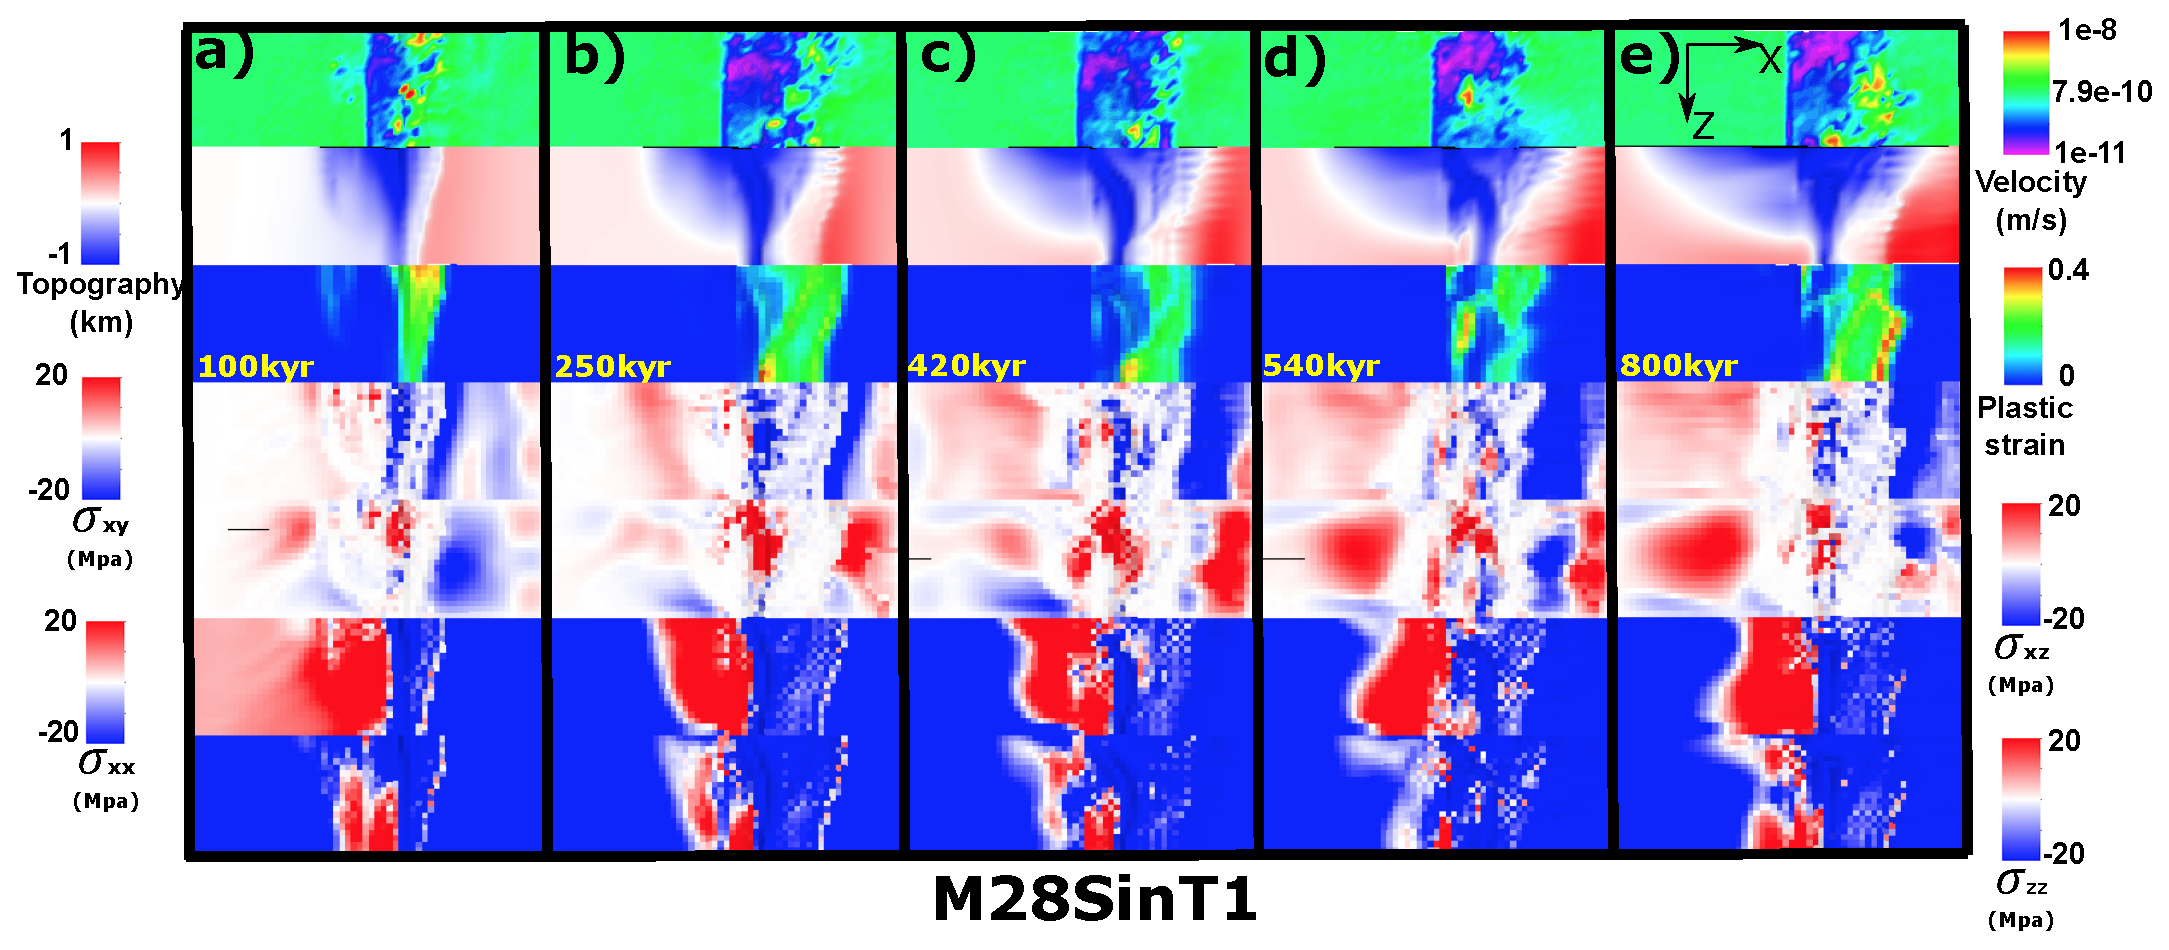
\includegraphics[width=1.0\textwidth]{./Figures/fig_Results_MRange_1_M28SinT1_time_evolution.eps}
 \caption{M28SinT1 (Table~\hyperref[Tab1_1]{\ref{Tab1_1}}) faulting and stress evolution with respect to time.}
\label{fig_Results_MRange_1}
\end{figure}

As shown in Figure~\hyperref[fig_Results_MRange_1]{\ref{fig_Results_MRange_1}}, faulting evolution is much less dynamic than that of M58SinT1. Faulting keeps on the right hand side of the ridge-axis. Only one secondary fault is formed at around 540kyr (Figure~\hyperref[fig_Results_MRange_1]{\ref{fig_Results_MRange_1}.d}). Initially, at 100kyr (Figure~\hyperref[fig_Results_MRange_1]{\ref{fig_Results_MRange_1}.a}), at the low Z side, the normal shear zone at conjugate plate takes up part of the extension and leave a dent in the topography. But it doesn't last long. The initial breakaway of the detachment extends further away from ridge-axis with four elements in along ridge-axis offset at 250kyr (Figure~\hyperref[fig_Results_MRange_1]{\ref{fig_Results_MRange_1}.b}). At 420kyr, at the high Z side, a hint of new near ridge-axis high angle normal fault begin to show up. It delvelop into a secondary fault at 540kyr (Figure~\hyperref[fig_Results_MRange_1]{\ref{fig_Results_MRange_1}.d}) and propagates toward high Z side. This results in a sinistral shear zone (red region in 5th row). At the low Z side (Z$=1\sim3$), a tensile failure can be seen and it take up part of the extension at the low Z side which results in the recede of termination at the low Z side as seen at 800kyr (Figure~\hyperref[fig_Results_MRange_1]{\ref{fig_Results_MRange_1}.e}) while the termination at higher Z side extends further away from the ridge-axis.

\subsubsection{M57SinT2 versus M58SinT2}
For description of M57SinT2 evolution with respect to time, please refer to Section~\hyperref[para_M57SinT2]{\ref{para_M57SinT2}} and Figure~\hyperref[fig_Results_Weakenging_4]{\ref{fig_Results_Weakenging_4}}. For description of M58SinT1 evolution with respect to time, please refer to  Section~\hyperref[para_M58SinT2]{\ref{para_M58SinT2}} and Figure~\hyperref[fig_Results_Weakenging_6]{\ref{fig_Results_Weakenging_6}}. A major difference is that M57SinT2 does not create alternating normal faults on each side of the ridge-axis while M58SinT2 does. \add[XT]{Why this seemingly small change could lead to such a to the first order difference in model behaviors?}

\subsubsection{M28LinT1 versus M57LinT1}
For description of M28LinT1 evolution with respect to time, please refer to Section~\hyperref[sec_M28LinT1]{\ref{sec_M28LinT1}}.
\paragraph{M57LinT1}\label{para_M57LinT1}

\begin{figure}[h]
 \centering
  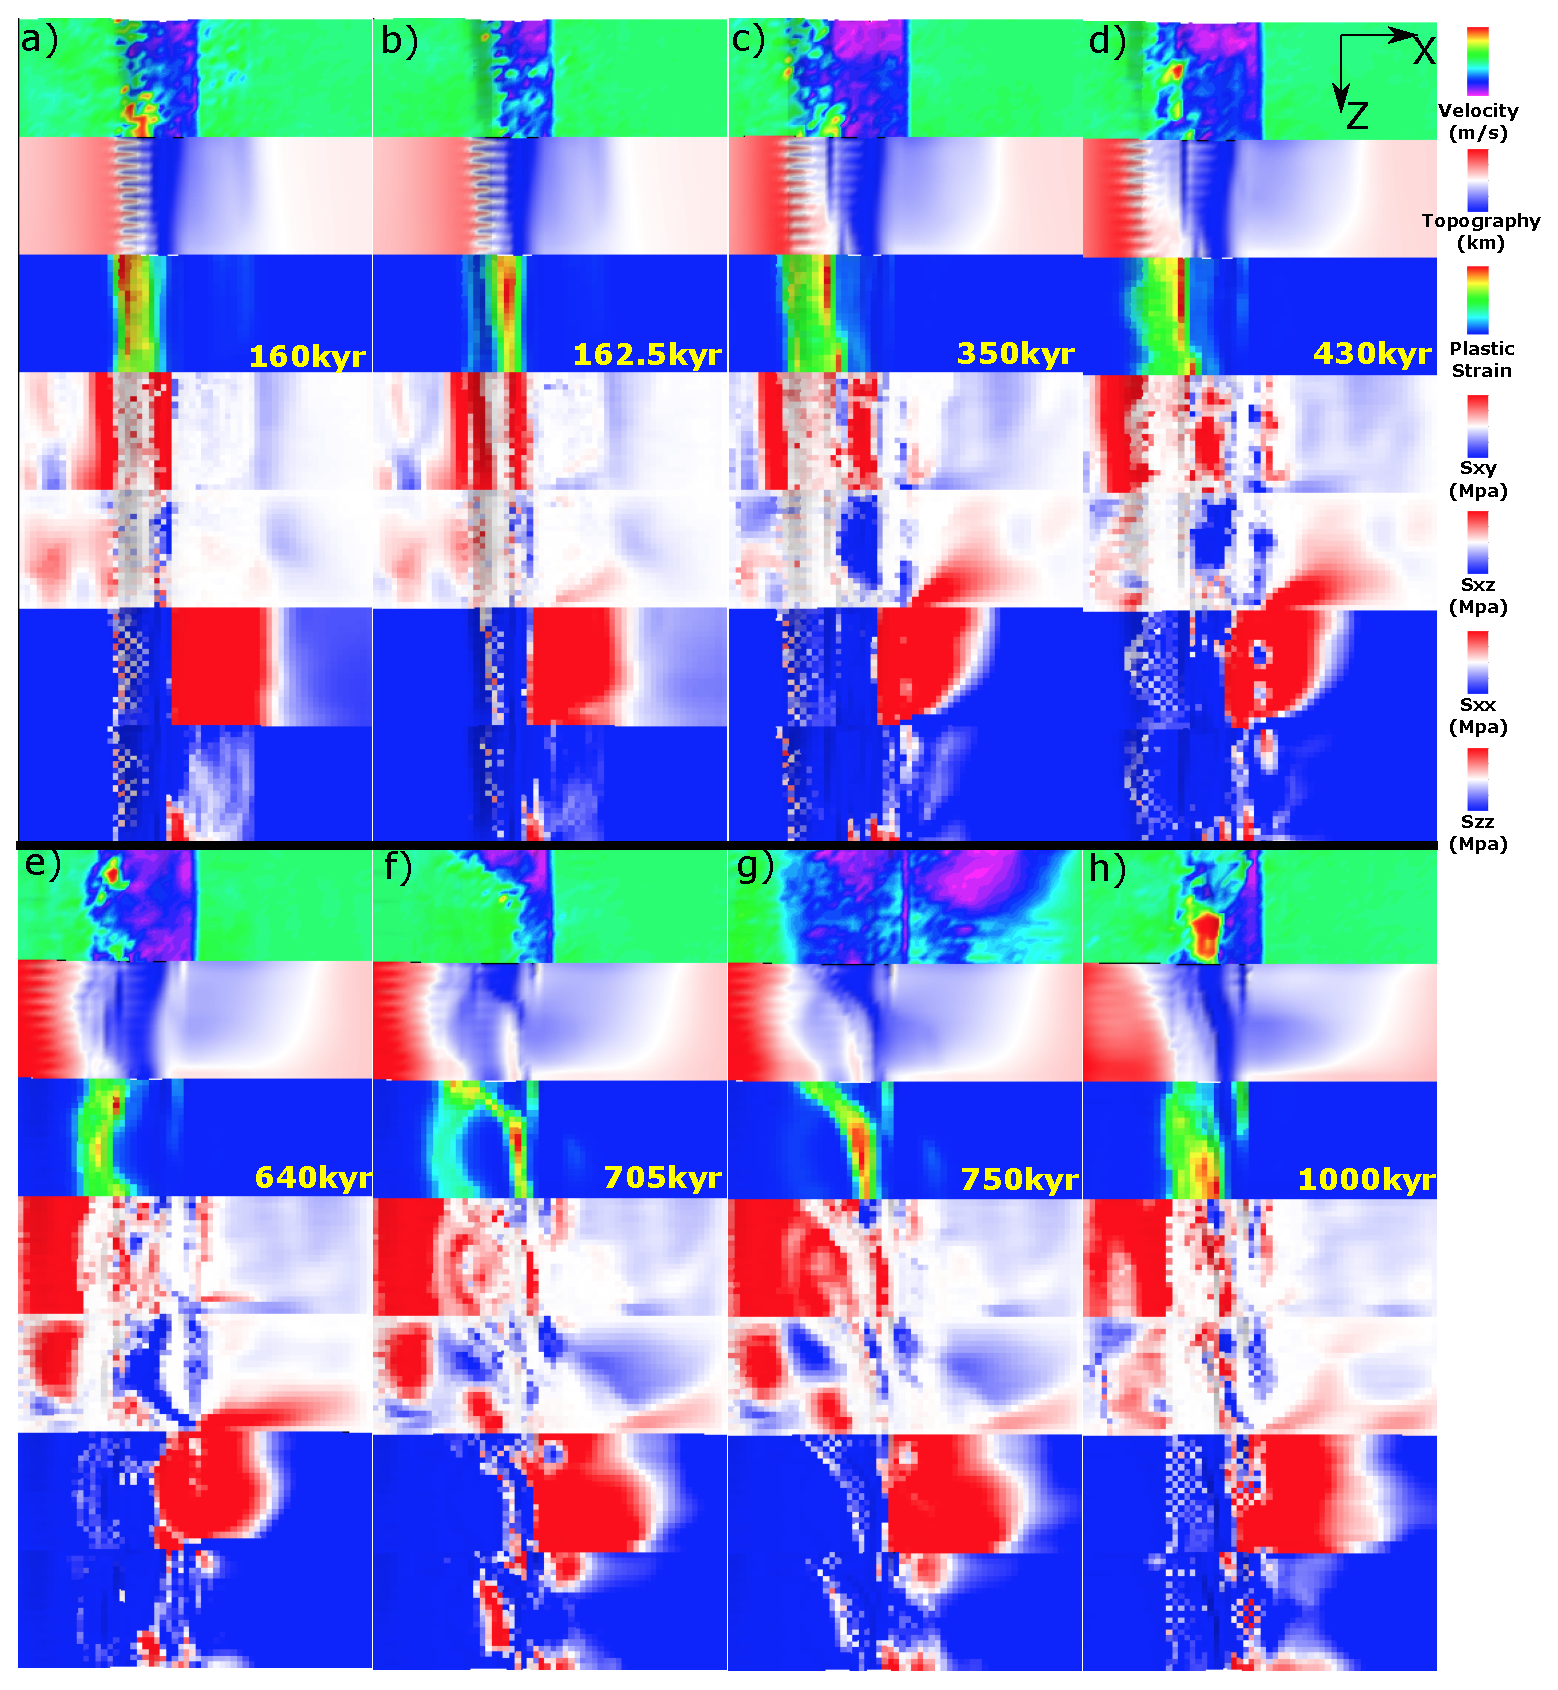
\includegraphics[width=0.8\textwidth]{./Figures/fig_Results_MRange_2_M57LinT1_time_evolution.eps}
 \caption{M57LinT1 (Table~\hyperref[Tab1_1]{\ref{Tab1_1}}) faulting and stress evolution with respect to time.}
\label{fig_Results_MRange_2}
\end{figure}

As shown in Figure~\hyperref[fig_Results_MRange_2]{\ref{fig_Results_MRange_2}}, between 160kyr (Figure~\hyperref[fig_Results_MRange_2]{\ref{fig_Results_MRange_2}.a}) and 162.5kyr (Figure~\hyperref[fig_Results_MRange_2]{\ref{fig_Results_MRange_2}.b}), there is a cut back. The corrugation is very severe and have a discrete distribution with one element width as its wavelength. The frontier of breakaway also shows discrete distribution of $\sigma_{xx}$ and $\sigma{zz}$ alternating between tension and compression which might be the reason for the undulating topography. At 350kyr (Figure~\hyperref[fig_Results_MRange_2]{\ref{fig_Results_MRange_2}.c} 3rd row), the two offsetted red line indicates tensile failure at the termination and the shorter one at the high Z side helps maintain a near ridge-axis high angle normal fault. At 430kyr (Figure~\hyperref[fig_Results_MRange_2]{\ref{fig_Results_MRange_2}.d}), the presence of vertical tensile failure near the ridge-axis at the low Z side is responsible for the recede of the front of the plastic strain at Z$=1\sim3$. While at Z=$5\sim10$, the breakaway keeps extending further away from the ridge-axis. This curved front results in a curved topography as seen in 640kyr (Figure~\hyperref[fig_Results_MRange_2]{\ref{fig_Results_MRange_2}.e}) and is also responsible for the large dextral shear (blue) zone (5th row). At 705kyr (Figure~\hyperref[fig_Results_MRange_2]{\ref{fig_Results_MRange_2}.f}), a new near ridge-axis secondary fault begin to evolve and replace the original one at high Z side with a length of $\sim15$ kilometers. The secondary fault also connect with the further away from ridge-axis original fault at low Z side. The topography at 1000kyr (Figure~\hyperref[fig_Results_MRange_2]{\ref{fig_Results_MRange_2}.h}) is a result of the curved and later connected fault. The frontier of the plastic strain at high Z side soon catch up with that at the low Z side due to the presence of a tensile failure zone a the low Z side that has taken up part of the extension.
       
\subsubsection{M28SqrtT1 versus M58SqrtT1}
For description of M28SqrtT1 evolution with respect to time, please refer to Paragraph~\hyperref[para_CutBack]{\ref{para_CutBack}} and Figure~\hyperref[fig_Results4_9]{\ref{fig_Results4_9}}.

For description of M58SqrtT1 evolution with respect to time, please refer to Paragraph~\hyperref[para_M58SqrtT1]{\ref{para_M58SqrtT1}} and Figure~\hyperref[fig_Results_Weakenging_7]{\ref{fig_Results_Weakenging_7}}.


\subsubsection{M57SqrtT2 versus M58SqrtT2}

For description of M58SqrtT2 evolution with respect to time, please refer to Paragraph~\hyperref[para_M58SqrtT2]{\ref{para_M58SqrtT2}} and Figure~\hyperref[fig_Results_Weakenging_8]{\ref{fig_Results_Weakenging_8}}.

The major difference between M57SqrtT2 and M58SqrtT2 is that M57SqrtT2 keeps faulting at the same side of the ridge-axis while M58SqrtT2 alternates.

\paragraph{M57SqrtT2}

\begin{figure}[h]
 \centering
  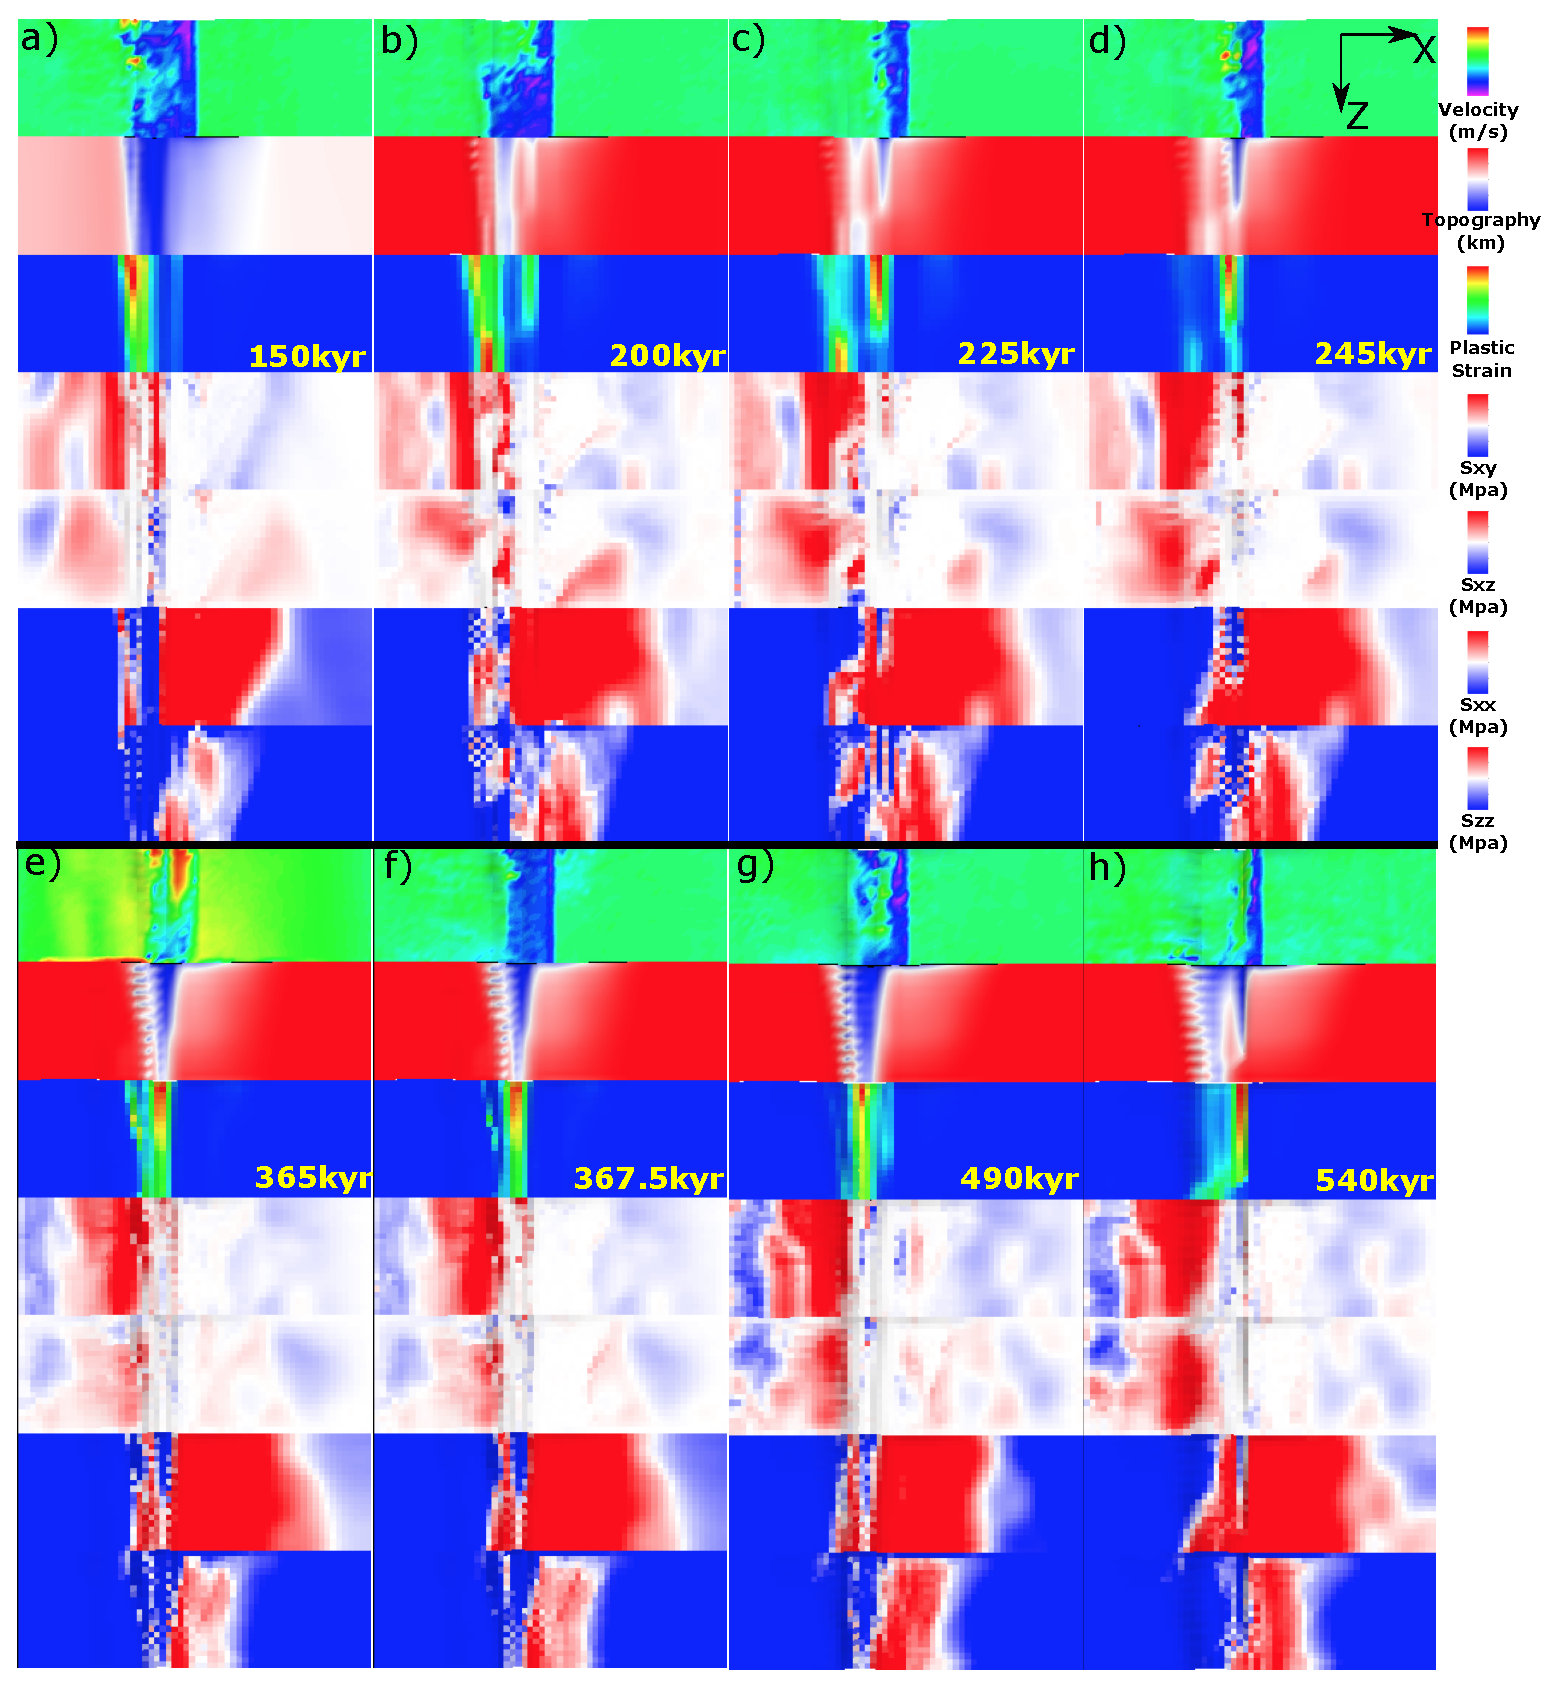
\includegraphics[width=0.8\textwidth]{./Figures/fig_Results_MRange_3_M57SqrtT2_time_evolution.eps}
 \caption{M57SqrtT2 (Table~\hyperref[Tab1_1]{\ref{Tab1_1}}) faulting and stress evolution with respect to time.}
\label{fig_Results_MRange_3}
\end{figure}

For M57SqrtT2, there are totally six small scale cut back happen at 282.5kyr, 290kyr, 365kyr, 452.5kyr, 482.5kyr and 540kyr respectively (the model stops at 540kyr). As shown in Figure~\hyperref[fig_Results_MRange_3]{\ref{fig_Results_MRange_3}}, the fault keeps on the left hand side of the ridge-axis. At 200kyr (Figure~\hyperref[fig_Results_MRange_3]{\ref{fig_Results_MRange_3}.b}), a new near ridge-axis high angle normal fault begin to evolve and take the place of the initial one. As the fault evolve, a transient stage of discontinuous abyssal hill is produced at the low Z side as seen at 225kyr (Figure~\hyperref[fig_Results_MRange_3]{\ref{fig_Results_MRange_3}.c}). The fault propagate toward high Z side and cut through the plate at $\sim$245kyr (Figure~\hyperref[fig_Results_MRange_3]{\ref{fig_Results_MRange_3}.d}) when sawtooth shape topography at the low Z side (2nd row) is created by sawtooth shape $\sigma_{xx}$ (6th row) and $\sigma_{zz}$ (7th row). Between 365kyr (Figure~\hyperref[fig_Results_MRange_3]{\ref{fig_Results_MRange_3}.e}) and 367.5kyr (Figure~\hyperref[fig_Results_MRange_3]{\ref{fig_Results_MRange_3}.f}), there is a cut back. At 490kyr (Figure~\hyperref[fig_Results_MRange_3]{\ref{fig_Results_MRange_3}.g}), there is new near ridge-axis antithetic fault on the hanging wall which terminates the old fault and develops into a vertical near ridge-axis tensile failure as seen at 540kyr (Figure~\hyperref[fig_Results_MRange_3]{\ref{fig_Results_MRange_3}.h}).

\subsection{Cut-back}

\subsection{Corrugations}
\subsubsection{Corrugations due to anastomosing}
\subsubsection{Corrugations due to asynchronous normal faulting}

\subsection{Summary of Results}
There are several behaviors that are controlled by the model parameters. Generally, only M58 models with Type two weakening produce aternating faults on both side of the ridge-axis. All the models show corrugations. As for faulting patterns in terms of evolution frequency, usually Square root is more dynamic than Sinusoidal than Linear, M58 is more dynamic than M57 than M28.

Following tables are a summery of the model behaviors with respect to different setup parameters.
 

\begin{table}[h]
\begin{small}
\begin{center}
\begin{tabular}{||l|l||l|l||l|l||}
\hline
A & Alternating Fault & C & Corrugation & SL & Shear Topography Low \\
\hline
NA& Not Alternating & SF & Secondary Fault on one side & CB & Cut Back   \\
\hline
DD &  Double Dome  & AM    & Atlantis Massif Shape &  &   \\
\hline
\end{tabular}
\end{center}
\end{small}
\caption{Model behaviors in short.}
\label{Tab1}
\end{table}

Based on the 11 models with M variation, we observed eight first-order behaviors as shown in Table~\hyperref[Tab1]{\ref{Tab1}}. 


\begin{table}[h]
\begin{small}
\begin{center}
\begin{tabular}{|l|p{3.5cm}|p{3.5cm}|p{3.5cm}|}
\hline
\diagbox[width=6em]{Type}{M range}&
M28&M57&M58\\
\hline
Type one &NA; C; SL; SF$_{1500kyr}$; DD    &NA; C; SF$_{1380kyr}$; CB$_{330kyr}$; AM(opposite z)     &    \\
\hline
Type two &    &     &    \\
\hline
\end{tabular}
\end{center}
\end{small}
\caption{Linear functional form.}
\end{table}

\begin{center}
\begin{table}[h!]
\begin{small}
\begin{tabular}{|l|p{3.5cm}|p{3.5cm}|p{3.5cm}|}
\hline
\diagbox[width=6em]{Type}{M range}&
M28&M57&M58\\
\hline
Type one & NA; C; SL; SF$_{995kyr}$ & NA; C; SL; SF$_{760kyr;1320kyr}$; CB$_{520kyr}$; AM & NA; C; SL; CB$_{510kyr}$; SF$_{760kyr;1140kyr;1990kyr}$   \\
\hline
Type two &    &NA; C; SL; SF$_{680kyr}$; CB$_{905kyr}$     & A$_{450kyr;600kyr}$; C(only at low M); CB$_{990kyr}$   \\
\hline
\end{tabular}
\end{small}
\caption{Sinusoidal functional form.}
\end{table}
\end{center}

\begin{table}[ht]
\begin{small}
\begin{center}
\begin{tabular}{|l|p{3.5cm}|p{3.5cm}|p{3.5cm}|}
\hline
\diagbox[width=6em]{Type}{M range}&
M28&M57&M58\\
\hline
Type one & NA; C; SL; CB$_{205kyr;330kyr;1025kyr}$   &      & NA; C$_{1770kyr}$(due to shear with dif wave length); SF$_{860kyr}$(high M); SF$_{1190kyr}$(low M)(Dog Bone); SF$_{1690kyr}$    \\
\hline
Type two &    & NA; C; SF$_{435kyr;1060kyr}$; CB$_{585kyr}$; CB$_{735kyr}$; CB$_{910kyr}$; CB$_{970kyr}$    & A$_{550kyr;920kyr}$; C; CB$_{400kyr}$    \\
\hline
\end{tabular}
\end{center}
\end{small}
\caption{Square root functional form.}
\end{table}

\pagebreak
\section{Discussion}

\subsection{Overview of model behaviors}

\begin{figure}[h]
  \centering
    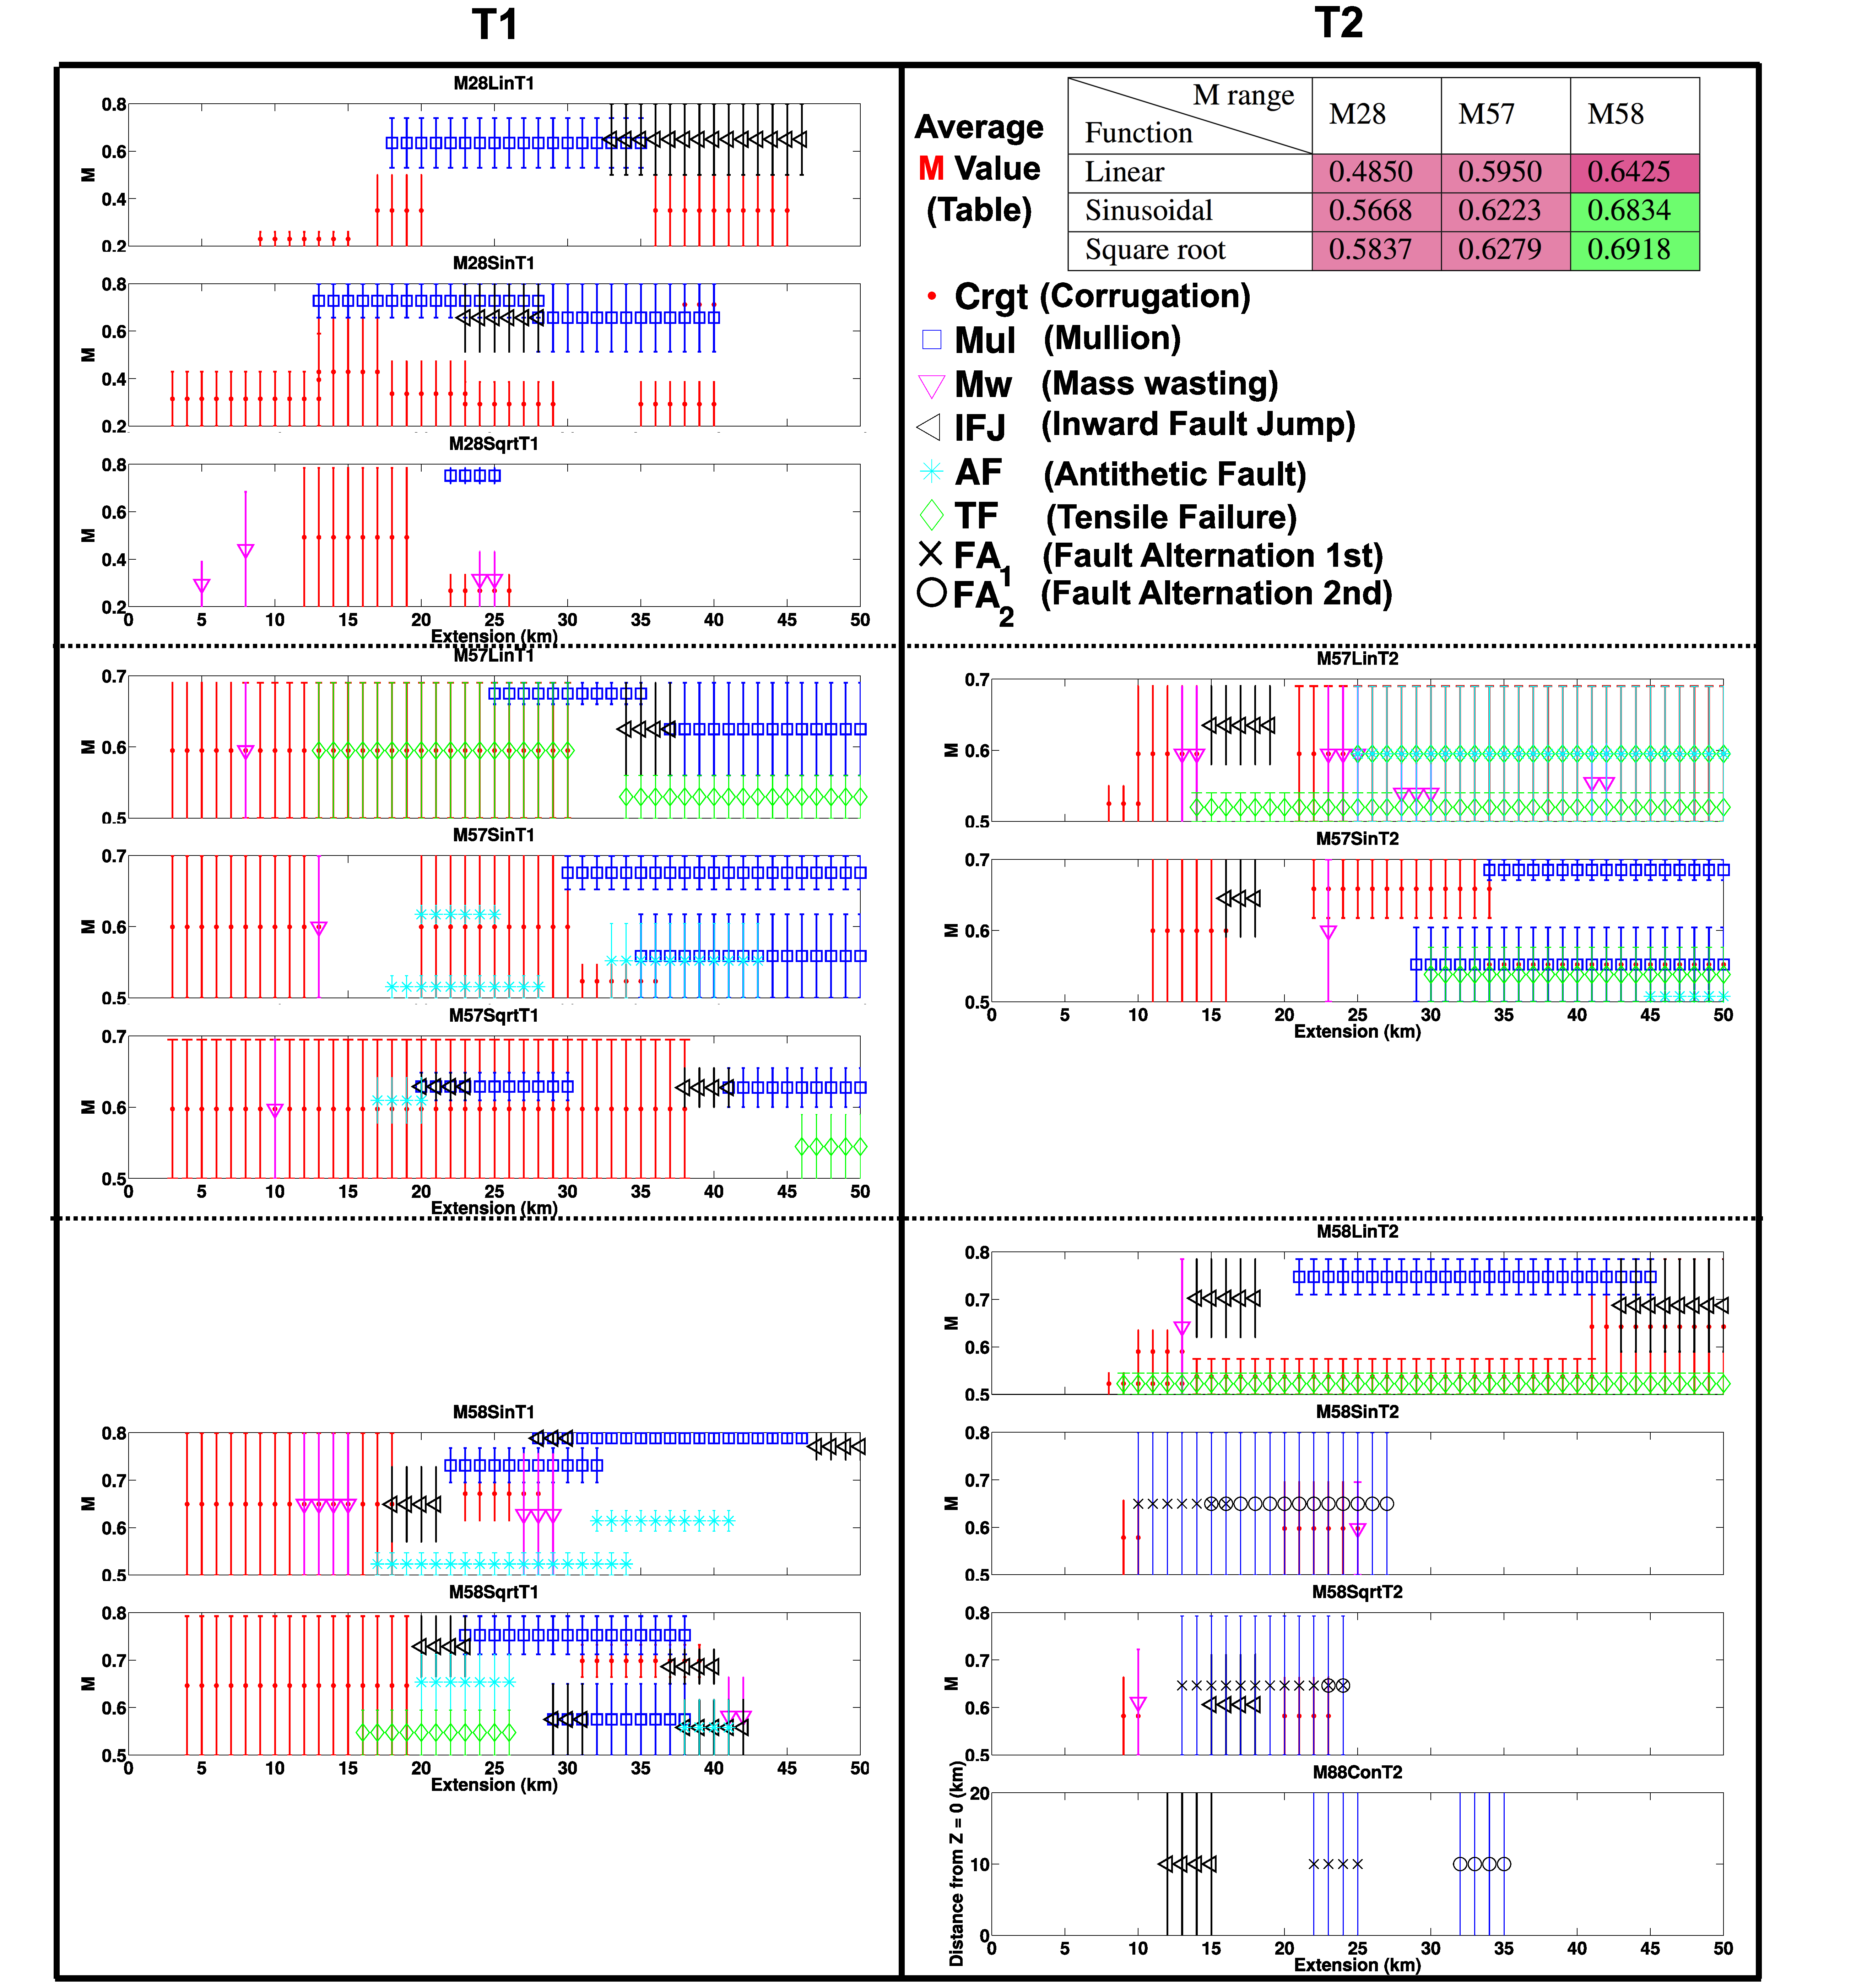
\includegraphics[width=1.0\textwidth]{./Figures/fig_Discussion_Result_Summary_1_Combine_together.eps}
    \caption{Initiation and duration of main structural features.}%\note[EC]{Labels of an individual plot are too small. Symbols can be bigger, too. You probably want to remove the table from this figure and keep it as a stand-alone table as I tried.}}
 \label{fig_Discussion_Result_Summary_1_Combine_together}
\end{figure} 

Model results show systematic changes with the average M value ($\bar{M}$), which is the integration of M along the ridge divided by the ridge length. $\bar{M}$ values of all the models are listed in Table~\hyperref[Tab_3_3_average_M]{\ref{Tab_3_3_average_M}}. $\bar{M}_{M58} > \bar{M}_{M57} > \bar{M}_{M28}$ and within each M range, $\bar{M}$ with sqaure root functional form is higher than that with sinusoidal form, which in turn is higher than the linear form.

%Only the M58 models with Type 2 weakening exhibit the fault alternation. However, the model with the linear M profile (M58LinT2) is an exception, which shows only an inward fault jump until the end of the model time, 1.1 Myr. The behaviors of this group of models indicate that there is an lower limit in the average M values with which fault alternation occurs. According to the tabulated values of M averaged over the along-ridge distance in Table~\hyperref[Tab_3_3_average_M]{\ref{Tab_3_3_average_M}}, the lower limit is between 0.6425 of M58LinT2 and 0.6834 of M58SinT2. Detailed analysis of the fault alternation is given in ``Discussion''. , 

To facilitate the challenging task of describing the complicated behaviors of each model as well as comparing different models, I visualize the model behavior as shown in Fig.~\hyperref[fig_Discussion_Result_Summary_1_Combine_together]{\ref{fig_Discussion_Result_Summary_1_Combine_together}}. Each plot has the amount of extension in km as the horizontal axis and M values as the vertical axis. The plot can succinctly show what structure appears, how long it takes to be created or remains active, and where it is created along the ridge. 
For instance, from the plot for M57SinT1 ($\bar{M} =$ 0.6223) in Fig.~\hyperref[fig_Discussion_Result_Summary_1_Combine_together]{\ref{fig_Discussion_Result_Summary_1_Combine_together}}, one can see that an antithetic fault first shows up after about 17 km of extension on the low M end, a mass wasting event occurs after about 13 km of extension and the inward fault jump is absent in this model. Similarly, the plot for the M57SqrtT1 model ($\bar{M} =$ 0.6279) clearly shows that this model experiences two inward fault jumps. %and each of them produces a curved toward ridge axis termination. The curved termination is responsible for the following small scale mullion structure.

%The antithetic fault at the lower M side helps to maintain a closer to ridge axis termination which results in a larger mullion structure (Figure~\hyperref[fig_Discussion_Observation_1_Tucholke1998]{\ref{fig_Discussion_Observation_1_Tucholke1998}.a}) at the lower M side and thus produces an OCC with a shape similar to the Atlantis Massif at 30 $\degree$N Mid-Atlantic Ridge. 

Models with type 1 weakening, on the left column of Figure~\hyperref[fig_Discussion_Result_Summary_1_Combine_together]{\ref{fig_Discussion_Result_Summary_1_Combine_together}}, show more complex and dynamic behaviors as $\bar{M}$ increases. In other words, more of the main structural characteristics are created and they tend to have a higher recurrence frequency as $\bar{M}$ increases. %when faulting (i.e. inward fault jump, antithetic fault) as well as other main model behaviors (i.e. corrugation, mullion, mass wasting, tensile failure) become more complex and dynamical with higher recurrence ferquencies.
%
For instance, %Comparing M28SinT1 and M28LinT1 shows that 
the inward fault jump occurs earlier and lasts a shorter period of time in M28SinT1 than in M28LinT1 due to a higher $\bar{M}$ of M28SinT1. Furthermore, among three models with M28T1, mass wasting occurs only in M28SqrtT1, the model with the highest $\bar{M}$ among these M28T1 models. 
%During the mass wasting, a curved fault scarp with $\sim$1 km relief is produced and it has a shape very similar to 13 $\degree$N, Mid-Atlantic Ridge (please refer to a detailed discussion in the next section). 
The trend of greater complexity for higher $\bar{M}$ continues in the group of M57T1 models. Corrugations are created earlier along the whole 20 km ridge segment than in the M28-T1 models. Unlike the M28T1 group, all three models in the M57-T1 group have mass wasting. %M57LinT1 ($\bar{M} =$ 0.5950), it begins to have tensile failure which releases tensional stress in the hanging wall and results in the delay of inward fault jump. 
The two M58 models have 3 or 4 inward fault jumps but the M57 models have at most two of them. Also, corrugations are created earlier in the M57 models than in the M58 ones, which suggests that corrugation favors a specific range of $\frac{\partial M}{\partial Z}$, not necessarily higher $\bar{M}$. Between M58SinT1 ($\bar{M} =$ 0.6834) and M58SqrtT1 ($\bar{M} =$ 0.6918), the major difference is M58SqrtT1 has twice inward fault jumps at the lower M side because M values are higher at the lower M side.

When comparing models with different weakening rates, the most obvious difference is that only type 2 models generates alternating faults. The models that exhibit the fault alternation do not create the mullion structure because the pattern of termination can not last long enough to produce the mullion structure. Also, they have neither tensile failure nor antithetic fault.

M58LinT2 ($\bar{M} =$ 0.6425) does not show the fault alternation, which suggests that not only the range of M (M58) but also the average M value along the ridge $\bar{M}$ are responsible for the fault alternation. This provides an upper limit of $\bar{M} =$ 0.6425 in our 3D models for producing long lasting detachment faults that can generate OCCs. Comparing M57T2 and M57T1 models show that M57T2 models generally have earlier inward fault jumps but later corrugations. For the model with constant M = 0.8 along the ridge axis, the inward fault jump and fault alternations have a period of $\sim$10 km of extension which is consistent with that of field observations. Corrugation, mullion structures, mass wasting, antithetic fault and tensile failure are not produced in constant M model M88ConT2 and it implies that varying M is necessary for producing those features.

\begin{figure}[h]
 \centering
  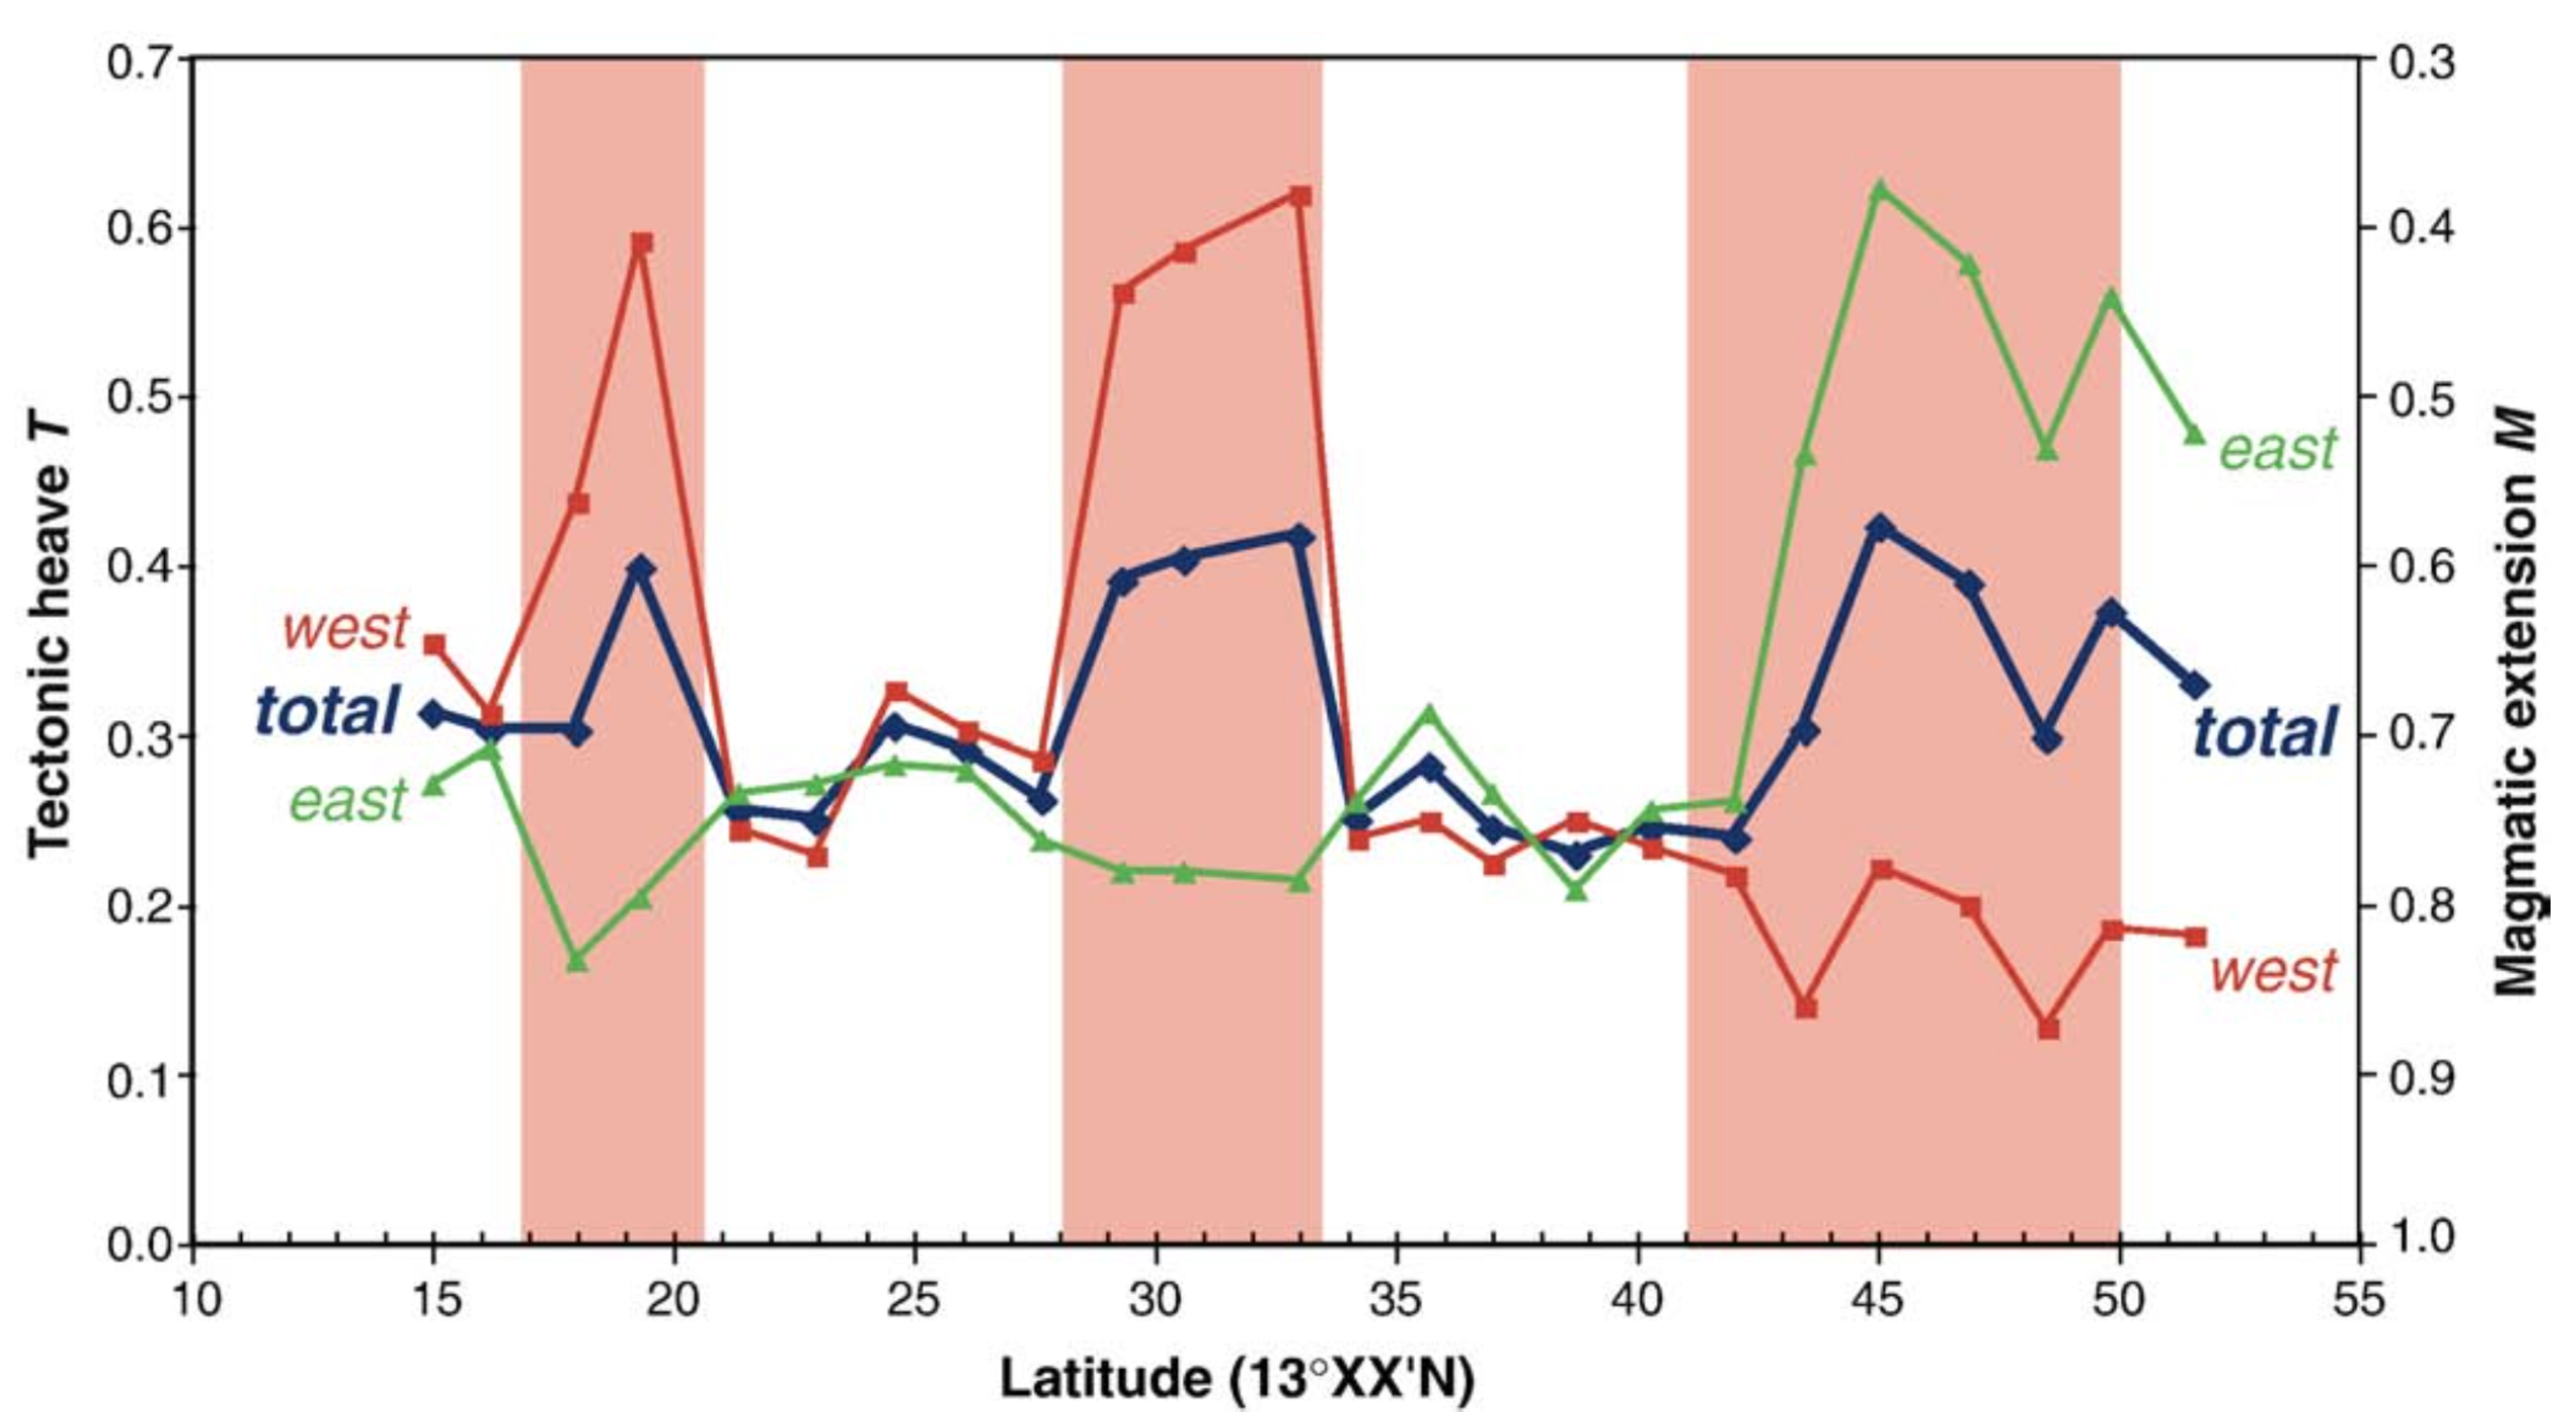
\includegraphics[width=1\textwidth]{./Figures/fig_Discussion_ResultsSummary_MacLeod2009.eps}
 \caption[Field observation results adapted from \citep{MacLeod2009}.]{Along-axis variations in total accumulated tectonic heave T in the past 1.86 Ma (since chron C2n), and consequent inferred magmatic component M (= 1 $-$ T) as a proportion of total plate separation (blue line). Pink shaded areas delineate loci of the active or recently active OCCs. The relative contributions of tectonic strain from the western and eastern flanks of the axis that give rise to the total heave T are shown by red and green lines respectively. Adapted from \citep{MacLeod2009}. }
 \label{fig_Discussion_ResultsSummary_MacLeod2009}
\end{figure}

In addition, the upper limit of $\bar{M} = $ 0.6425 for allowing a long lasting detachment fault to produce an OCC in our model is consistent to the results from a near-bottom sidescan bathymetric profiler survey and sampling study of the Mid-Atlantic Ridge near 13 $\degree$N \citep{MacLeod2009}. As shown in Figrure~\hyperref[fig_Discussion_ResultsSummary_MacLeod2009]{\ref{fig_Discussion_ResultsSummary_MacLeod2009}}, the average M value $\bar{M} =$ 0.63 $\pm$ 0.05 for the pink area where OCCs are present whereas when there is no OCC, $\bar{M} =$ 0.73 $\pm$ 0.03.

Under similar physical conditions of our model setup (e.g. thermal structure, rheology relationship, spreading velocity, weakening rate), the upper limit of $\bar{M} = $ 0.6425 predicts a boundary value between two observed morphological end members for slow spreading ridges: 1) long wavelength OCCs generated by a detachment fault; 2) high frequency abyssal hills results from symmetrical spreading of alternating high angle normal faults. Although the number of $\bar{M} = $ 0.6425 is highly consistent with natural observation (e.g. \citep{MacLeod2009}), we still need more works for a comprehensive result because model parameter such as viscosity of the underlying asthenosphere also contributes to whether fault alternates. For example, \citep{Allken2012} shows that higher value of viscosity of the ductile asthenosphere leads to better coupling between crust and mantle and promotes distributed muliple faulting rather than a focused long-lived detachment fault.

Previous 2D studies suggest that OCCs are most likely to form when M = 0.3 $\sim$ 0.5 [\citealp{Buck2005};\citealp{Tucholke2008}]. However, conflicts exist between model prediction and nature observation in both the upper and lower limits. For the upper limit conflict that OCCs are observed with M $>$ 0.5, \citet{Olive2010} suggests an explanation from a 2D model study that magma supplied in the ductile lower crust and upper mantle will not affect the faulting pattern and thus allows OCCs to be created under excessive diking. However, our 3D model results provides an alternative explanation that due to the along ridge coupling (i.e. torsion and shear), the region (M = 0.3 $\sim$ 0.5) along the ridge that promotes stable spreading by detachment faulting helps maintain the normal fault outside the region along the ridge. Once the detachment fault initiates along the whole ridge segment, it is very hard to modify the faulting pattern especially for a faster weakening rate (type 1). Thus, the detachemnt fault at the higher M side (M $>$ 0.5) can still last for more than 20 km of plates separation (Figure~\hyperref[fig_Discussion_Result_Summary_1_Combine_together]{\ref{fig_Discussion_Result_Summary_1_Combine_together}.M28LinT1}) before the fault alternation or inward fault jump ceases the exhuming process of the ultramafic mantle rocks. This along ridge coupling can also explain the conflict at the lower limit end when OCC is produced with observed M $<$ 0.3 (e.g., \citealp{Dick2008}; \citealp{Grimes2008}; \citealp{Baines2008}). Our 3D result suggests an extended range of M for OCCs formation than previous 2D studies (M = 0.3 $\sim$ 0.5) [\citealp{Buck2005};\citealp{Tucholke2008}]. 


\subsection{Comparing model results with natural observations}

%In this section, I compare the model behaviors with nature observations in terms of the following major model features: inward fault jump, fault alternation, mass wasting, hourglass shape median valley, mullion structure and corrugation.

\subsubsection{Inward fault jump}
\begin{figure}[h]
 \centering
  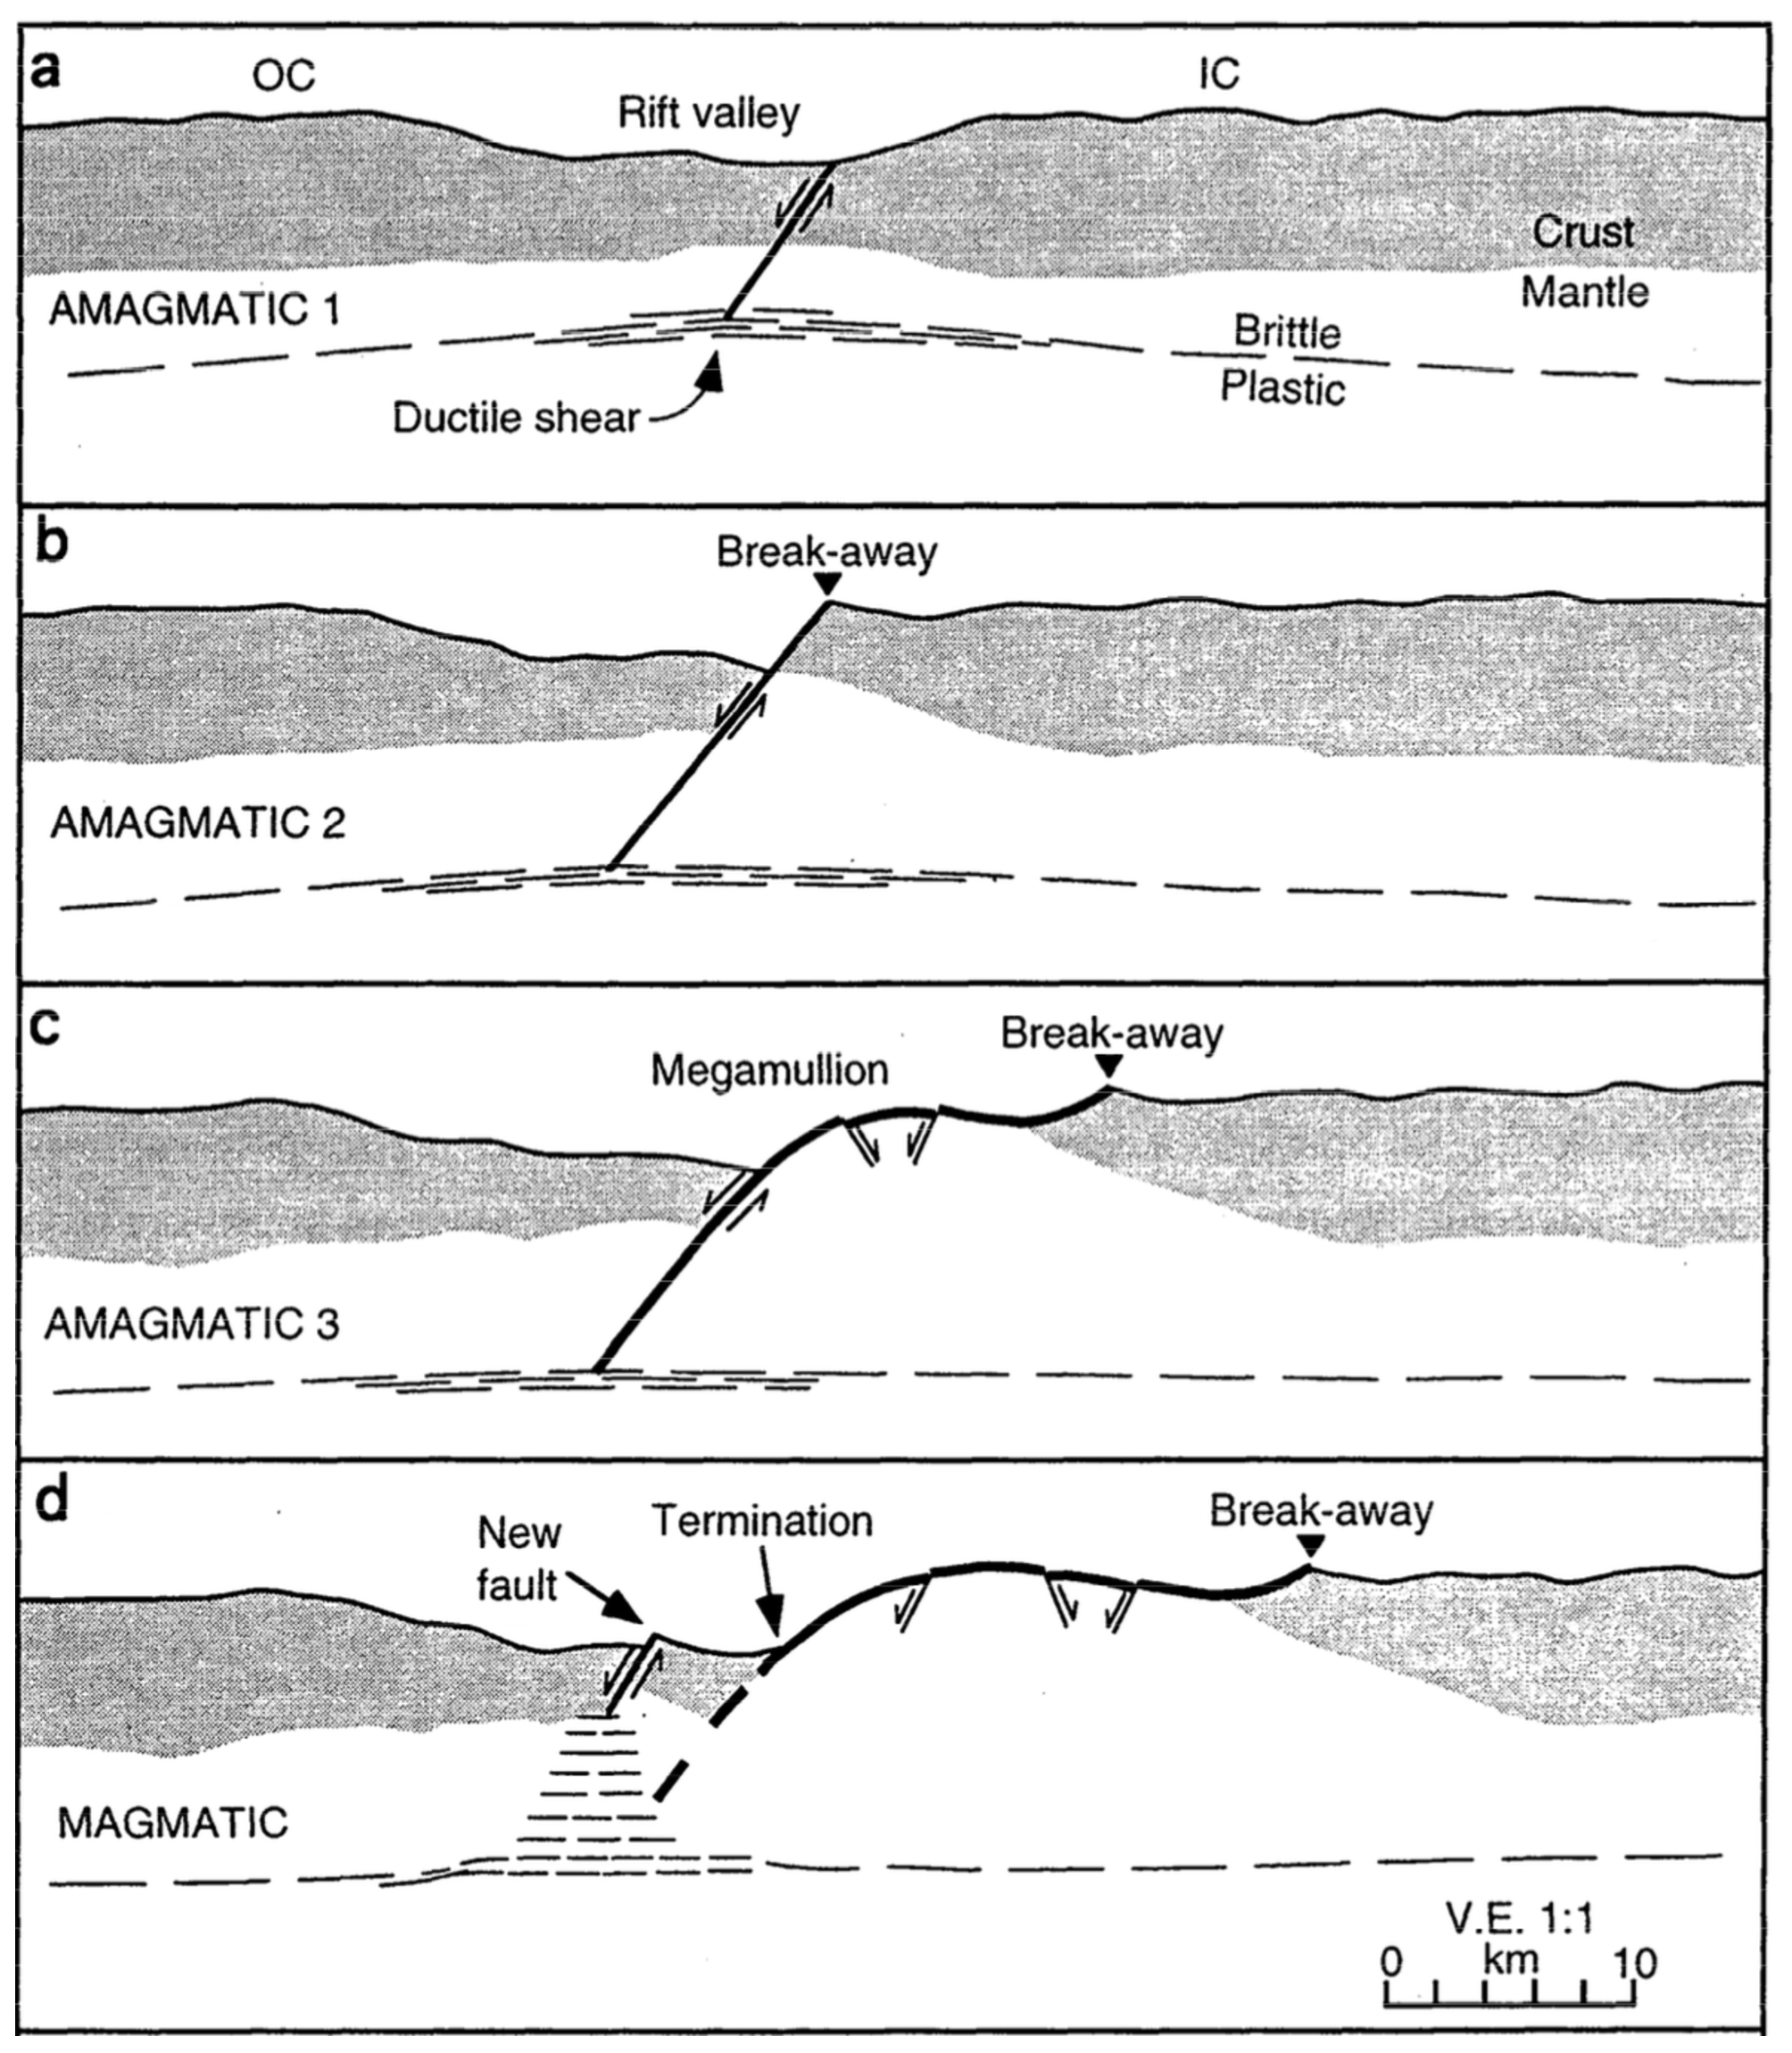
\includegraphics[width=0.7\textwidth]{./Figures/fig_Discussion_Observation_1_Tucholke1998.eps}
 \caption[Schematic development of a megamullion from amagmatic to magmatic, adapted from \citep{Tucholke1998}.]{Schematic development of a megamullion. No vertical exaggeration. (a)$\sim$(c) shows the detachment fault evolution during amagmatic phase. (d) Increased magma supply pushed the detachment fault away from ridge axis and forms a new normal fault near the ridge axis (``inward fault jump''). Adapted from \citep{Tucholke1998}.}
 \label{fig_Discussion_Observation_1_Tucholke1998}
\end{figure}

The term ``inward fault jump'' is first suggested in a study of geological and geophysical data from the Mid-Atlantic Ridge \citep{Tucholke1998}. It is the end phase of a general evolution of an OCC as is illustrated in Figure~\hyperref[fig_Discussion_Observation_1_Tucholke1998]{\ref{fig_Discussion_Observation_1_Tucholke1998}}. In the begining of a long amagmatic phase (Figure~\hyperref[fig_Discussion_Observation_1_Tucholke1998]{\ref{fig_Discussion_Observation_1_Tucholke1998}.a$\sim$c}) of seafloor spreading, a high angle normal fault cuts throught the brittle lithosphere and roots in the brittle-ductile transition (BDT) (Figure~\hyperref[fig_Discussion_Observation_1_Tucholke1998]{\ref{fig_Discussion_Observation_1_Tucholke1998}.a}). When the fault keeps slipping, the breakaway moves off axis and the fault begin to rotate to a lower dip angle (Figure~\hyperref[fig_Discussion_Observation_1_Tucholke1998]{\ref{fig_Discussion_Observation_1_Tucholke1998}.b}). Then, the exposed fault surface roll over and as the detachment fault keeps exhuming lower crust and upper mantle rocks, it generates a dome shape megamullion (OCC). The high angle normal faults cut the detachment fault surface where it is exposed to the seafloor is probably caused by the bending stresses during footwall roll over (Figure~\hyperref[fig_Discussion_Observation_1_Tucholke1998]{\ref{fig_Discussion_Observation_1_Tucholke1998}.c}). Then, when magma supply at the ridge center increases and pushes the detachment fault away from the ridge axis, the OCC formation is terminated by the new fault near the ridge axis which is termed as the ``inward fault jump''. As shown in the figure, initially, the footwall of this new fault is mostly composed of crust material like basalt, however, if this new fault can last a long period of time, it can also exhume lower ultramafic material.

\begin{figure}[h]
 \centering
  \includegraphics[width=1.0\textwidth]{./Figures/fig_Discussion_Observation_2_Dick2008_Kane.eps}
 \caption[Bathymetric map and simplified tectonic interpretation of Kane Megamullion. Adapted from \citep{Dick2008}.]{Bathymetric map and simplified tectonic interpretation of Kane Megamullion. Contour interval is 100 m. Pie diagrams show lithologic proportions by weight in dredge and dive collections. Detachemtn fault breakaway and termination are marked as dashed lines. Shaded regions indicate areas of possible off-axis volcanism. Adapted from \citep{Dick2008}.}
 \label{fig_Discussion_Observation_2_Dick2008_Kane}
\end{figure}

In our model, most of the inward jumping faults last less than 5 km of plates extension before the mantle materials can be exhumed to the seafloor. However, the M28LinT1 model produces an inward fault jump lasts for $\sim$15 km of extension (Figure~\hyperref[fig_Discussion_Result_Summary_1_Combine_together]{\ref{fig_Discussion_Result_Summary_1_Combine_together}.M28LinT1}) and produces a dome-shaped OCC ajacent to the initial one further way from the ridge axis (Figure~\hyperref[fig_Results1_1]{\ref{fig_Results1_1}.h}). This behavior might explain the formation mechanism of the brother Abel and Cain domes of the Kane megamullion at 23 $\degree$N MAR. As shown in Figure~\hyperref[fig_Discussion_Observation_2_Dick2008_Kane]{\ref{fig_Discussion_Observation_2_Dick2008_Kane}}, our model behaviors are consistent with the nature observation in terms of the breakaway and the wavelength of the domes assuming M decreases form south to north along the ridge axis. First of all, the breakway of the detachment fault is further away from the ridge axis at the northern than the sourthern end. Second, the Abel and Cain domes are larger than the Adam and Eve domes because the inward fault jump lasts longer at where M is relatively lower.    

\begin{figure}[h]
 \centering
  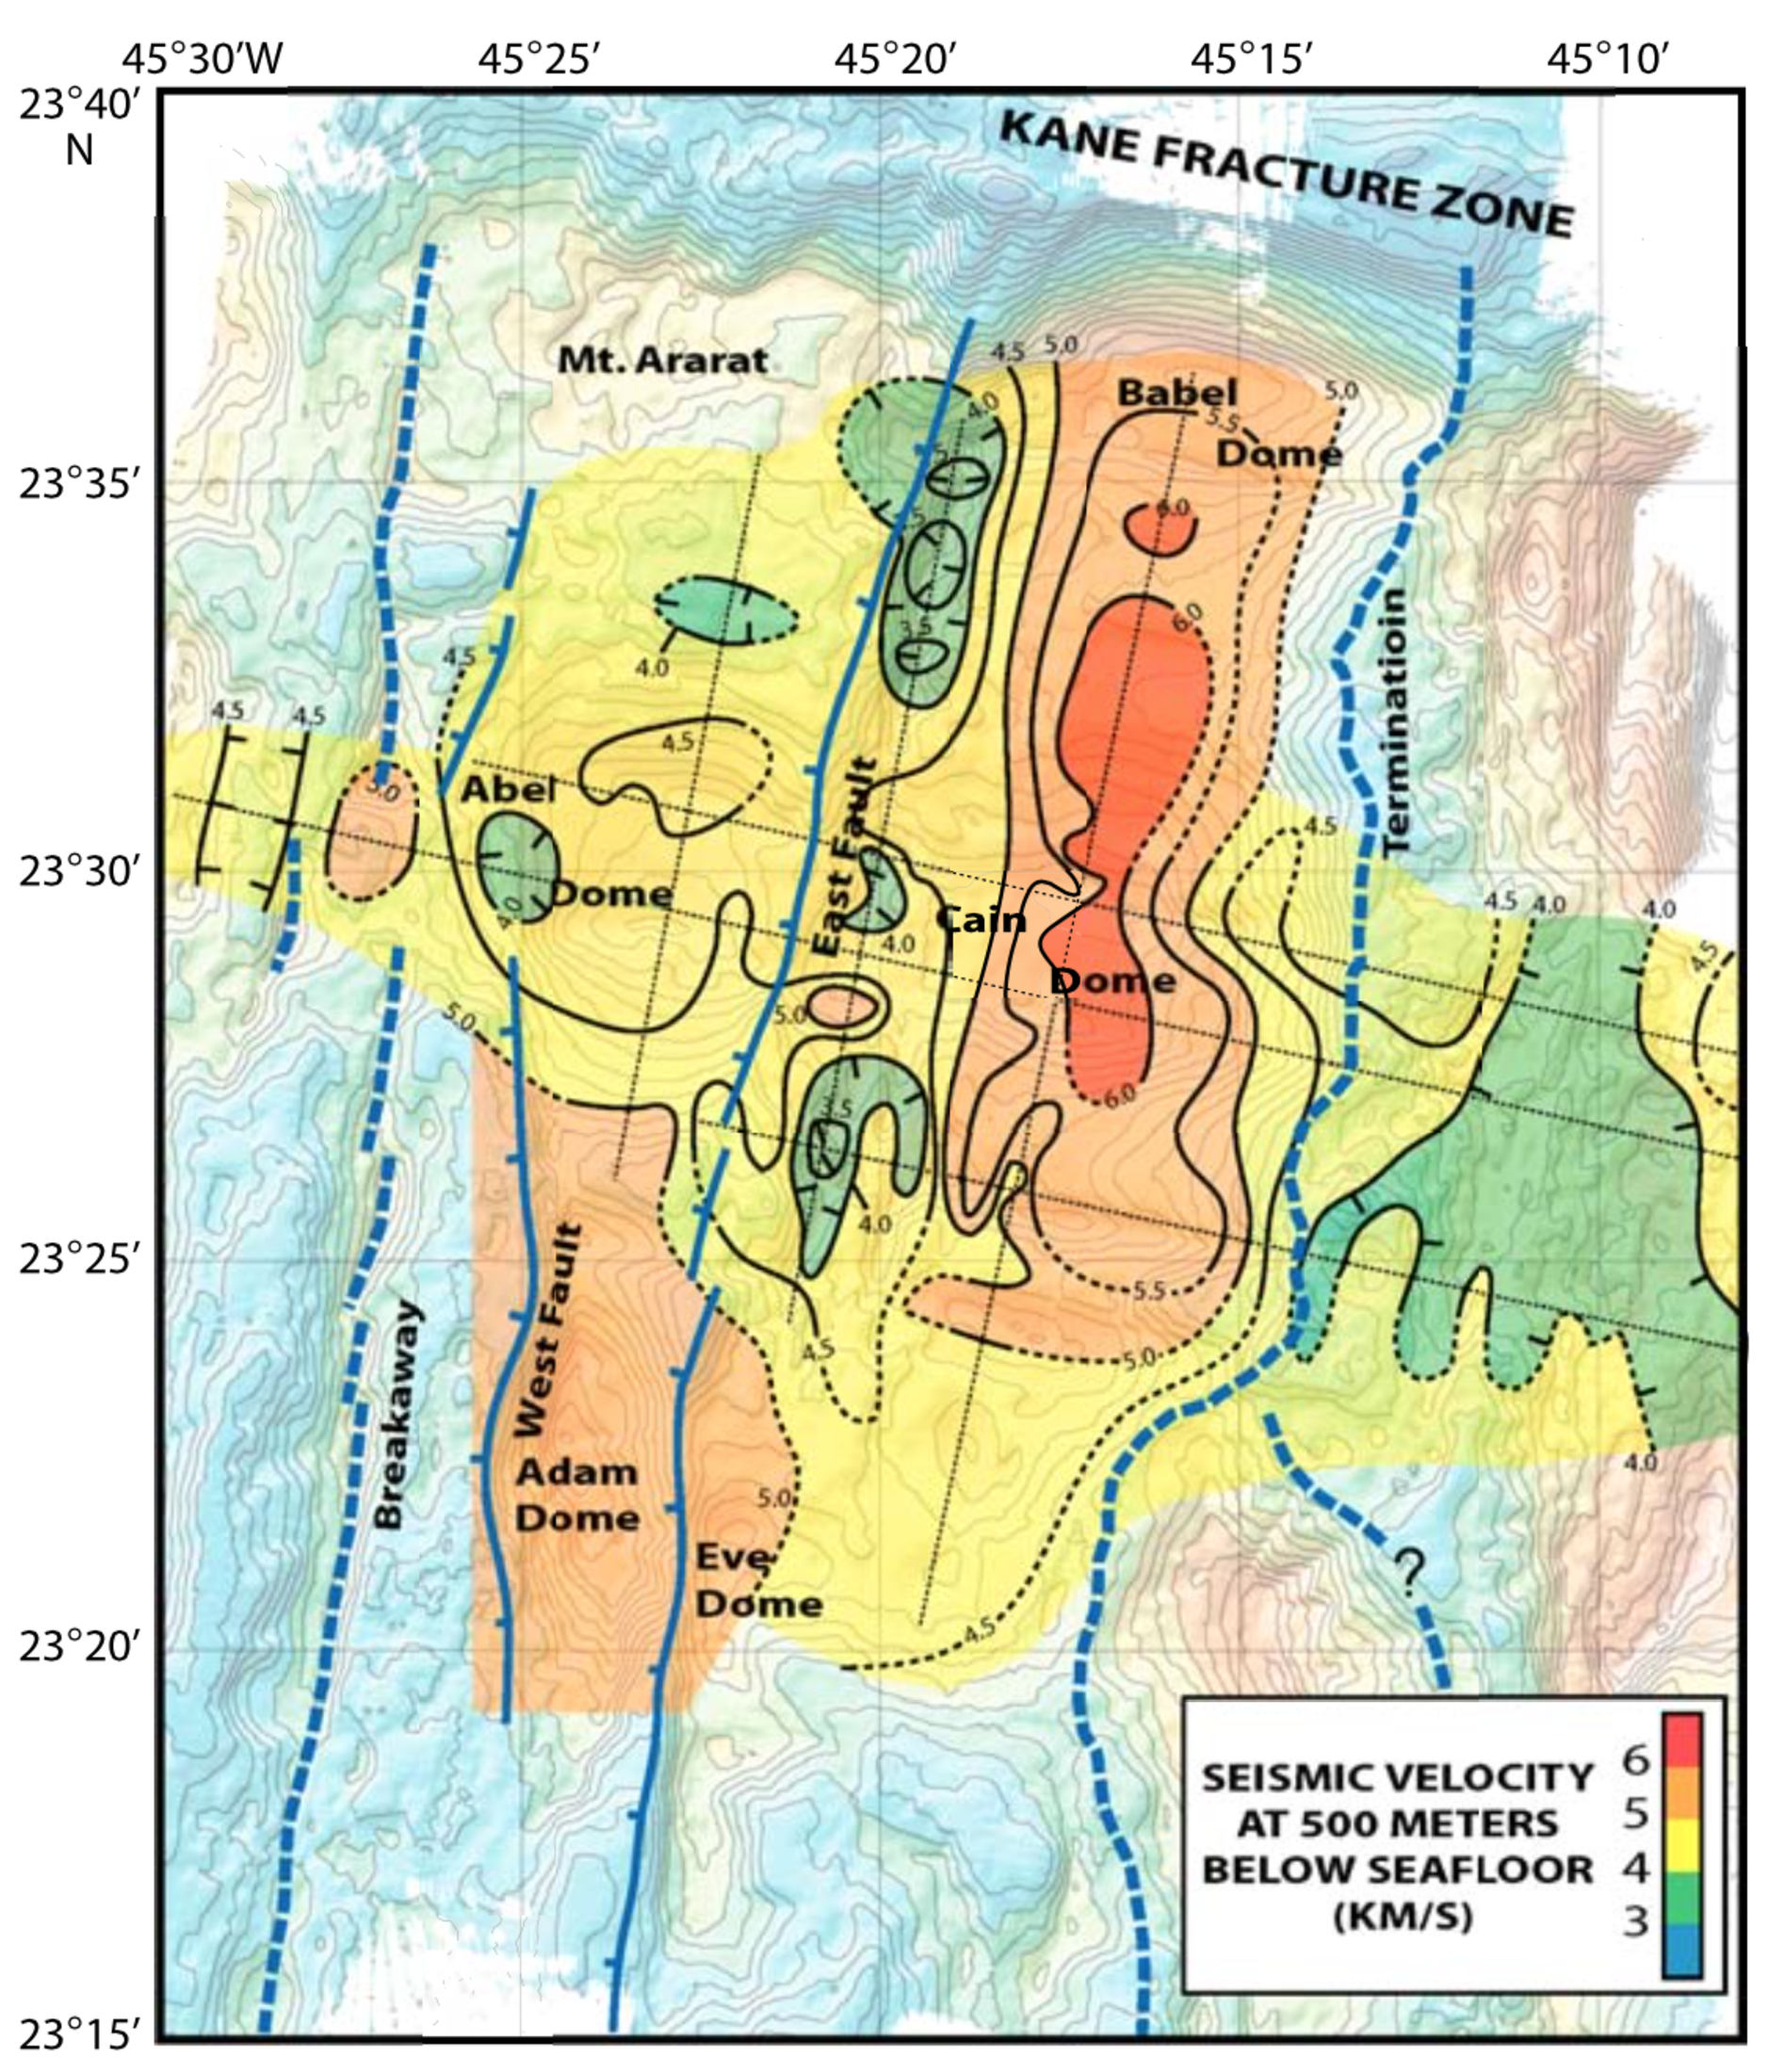
\includegraphics[width=0.6\textwidth]{./Figures/fig_Discussion_Observation_1_Xu2009_SeismicV_Kane.eps}
 \caption{P wave isovelocity contours at 500 m below seafloor superimposed on bathymetry and simplified tectonic interpretation. Adapted from \citep{Xu2009}.}
 \label{fig_Discussion_Observation_1_Xu2009_SeismicV_Kane}
\end{figure}

A seismic study \citep{Xu2009} showed that the Kane OCC is terminated at around 2.1 Myr ago when an eastward fault jump occured, i.e. when a new normal fault formed in the rift valley and captured a segment of the basaltic hanging wall. The velocity structure from their P wave tomography study verifies that the hanging wall block eastern to the Cain dome has a lower velocity corresponds to basaltic rocks (Figure~\hyperref[fig_Discussion_Observation_1_Xu2009_SeismicV_Kane]{\ref{fig_Discussion_Observation_1_Xu2009_SeismicV_Kane}}).

\subsubsection{Fault alternation}

\begin{figure}[h]
 \centering
  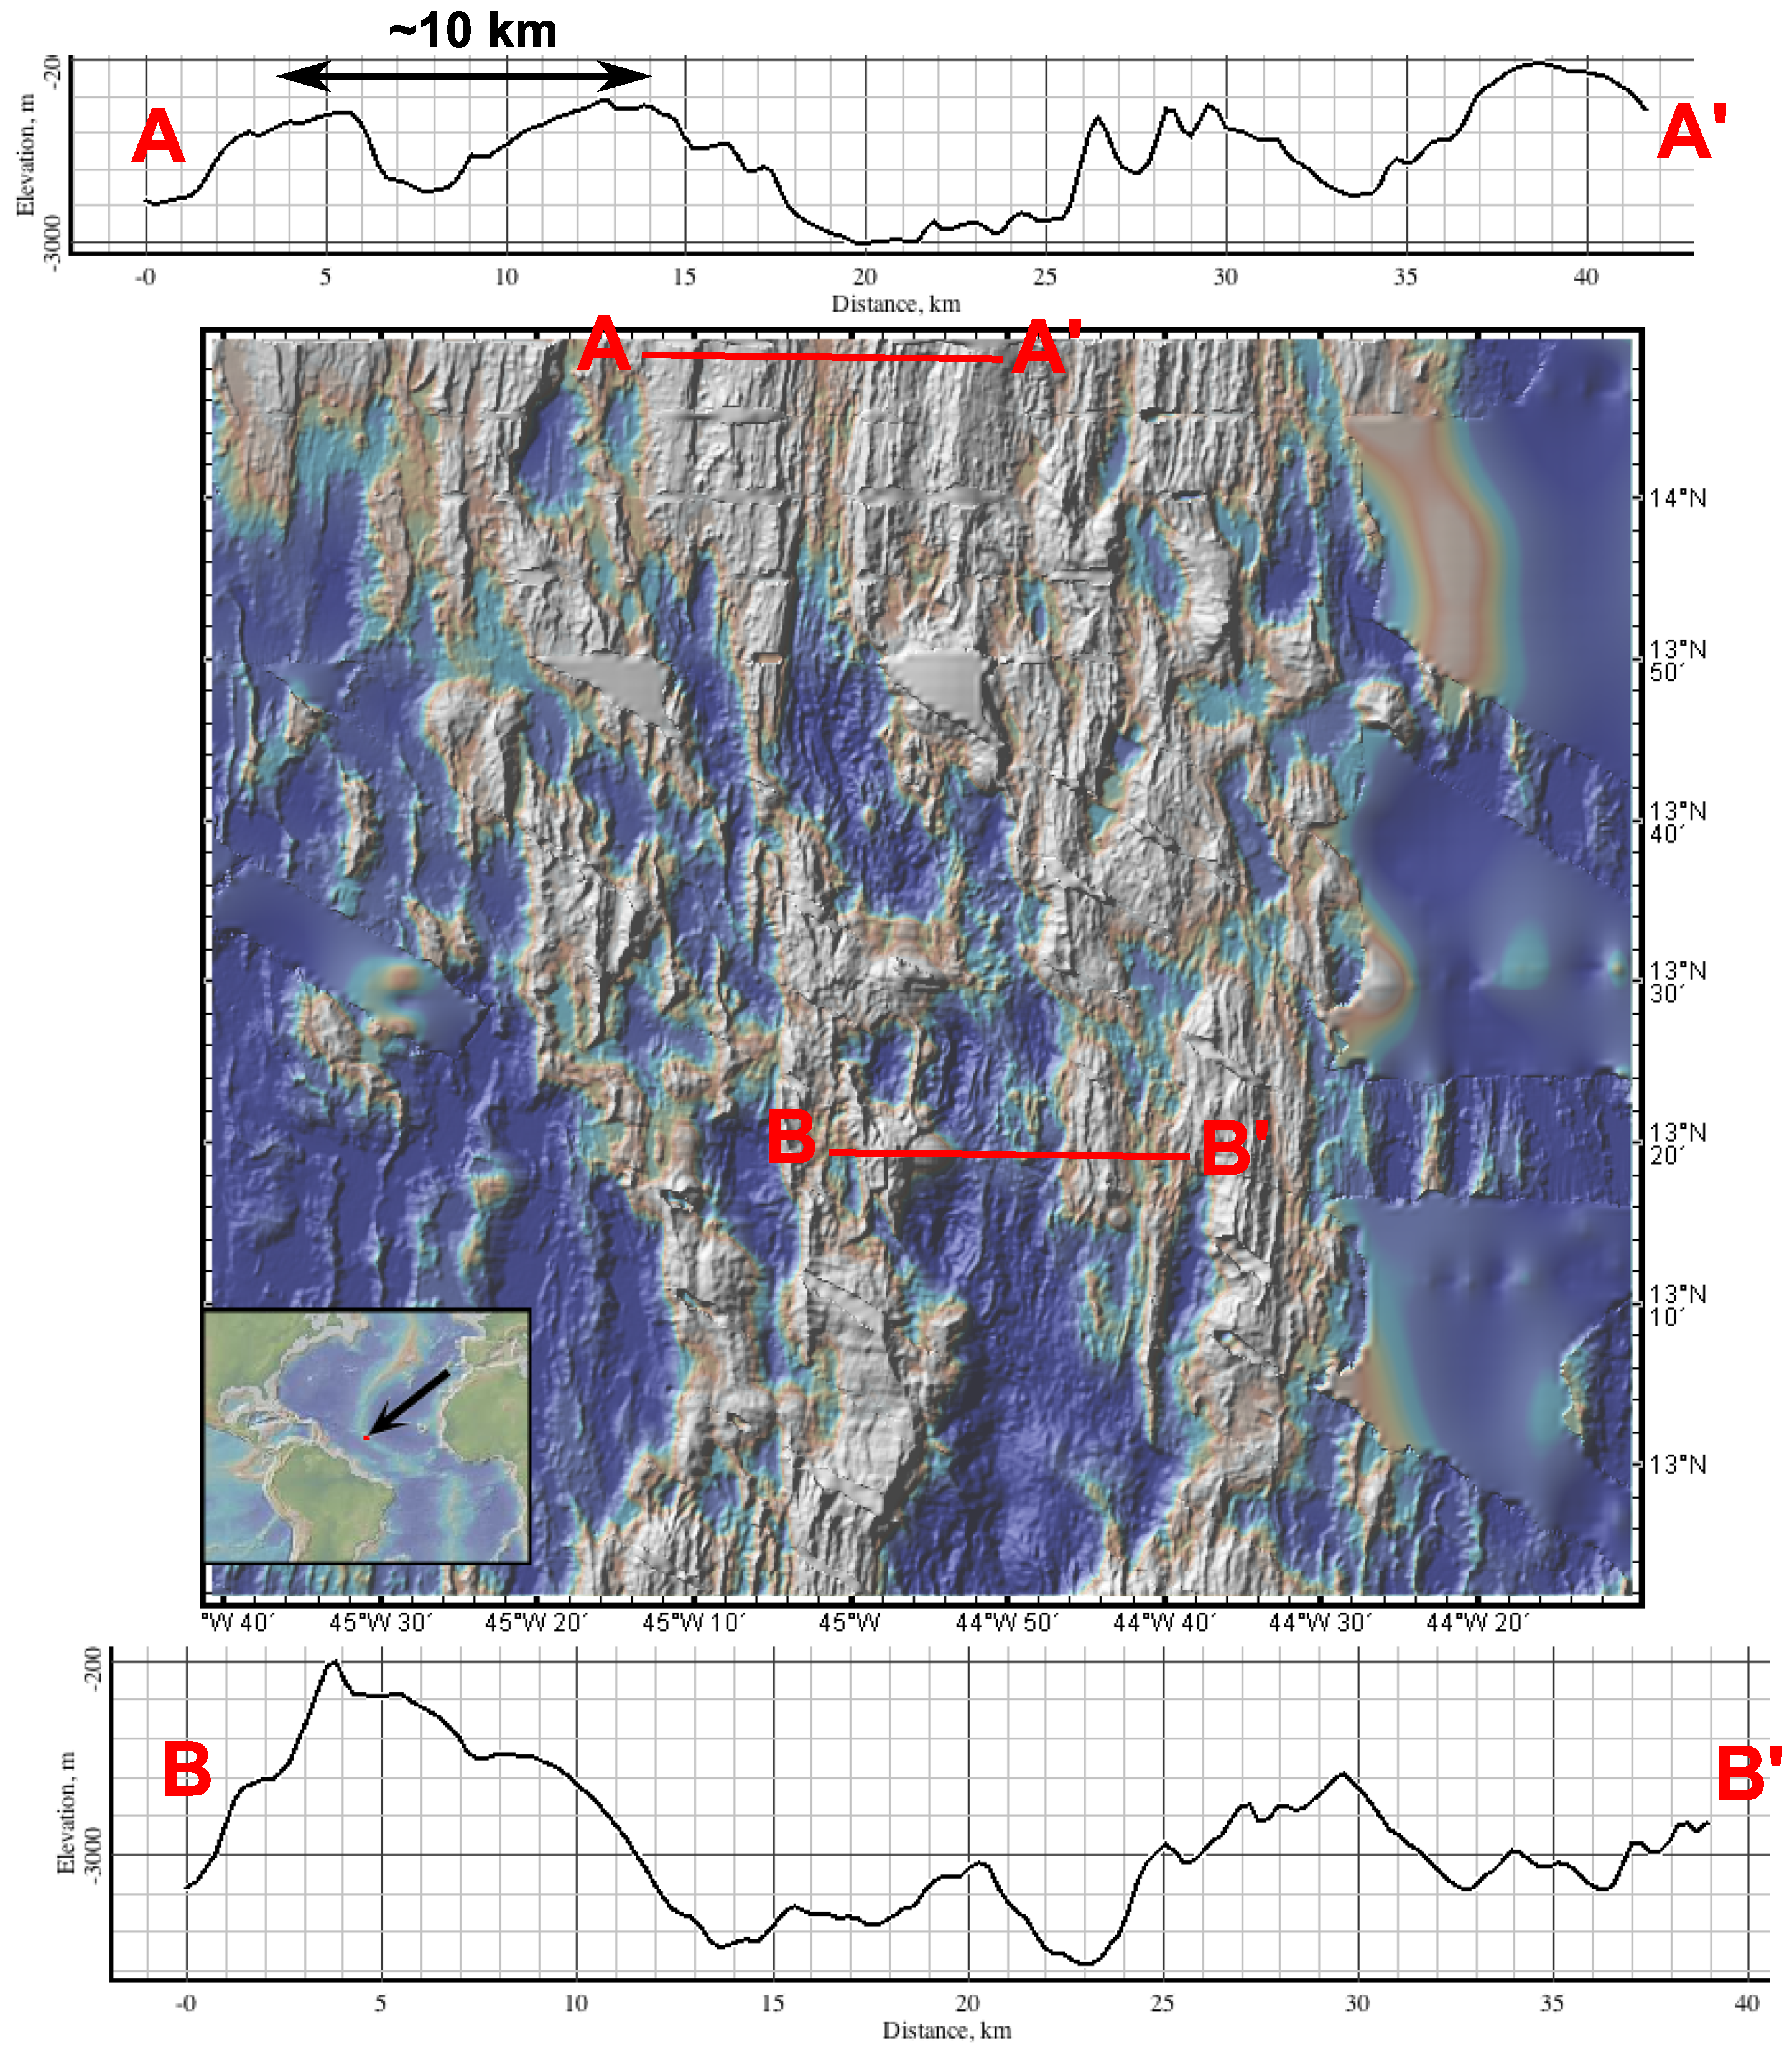
\includegraphics[width=0.75\textwidth]{./Figures/fig_Discussion_Observation_2_13-14N_MAR.eps}
 \caption[Bathymetry from 12.8$\sim$14.2 $\degree$N Mid-Atlantic Ridge.]{Bathymetry from 12.8$\sim$14.2 $\degree$N Mid-Atlantic Ridge. Crossection A$\sim$A$^{\prime}$ and B$\sim$B$^{\prime}$ are 5 times vertical exagerated. From GeoMapApp.}
 \label{fig_Discussion_Observation_2_13-14N_MAR}
\end{figure}

For slow-to-intermediate spreading ridges, the off-axis morphologies have two end members. One is the high-frequency abyssal hills that are relatively symmetrical across the ridge axis. They are usually found closer to the ridge segment center (crossection A-A$^{\prime}$ in Figure~\hyperref[fig_Discussion_Observation_2_13-14N_MAR]{\ref{fig_Discussion_Observation_2_13-14N_MAR}}). The other is the long wavelength asymmetrically spreading OCCs (crossection B-B$^{\prime}$ in Figure~\hyperref[fig_Discussion_Observation_2_13-14N_MAR]{\ref{fig_Discussion_Observation_2_13-14N_MAR}}). What is the mechanism for this distinct difference along the ridge? The fault alternation behavior in our model provides a 3D perspective for answering the question. When $\bar{M}$ is higher than 0.6425 with slower weakening rate (type 2), high frequency abyssal hills are generated. For example, M88ConT2 produces abyssal hills with $\sim$10 km in wavelength due to fault alternation (Figure~\hyperref[fig_Discussion_Result_Summary_1_Combine_together]{\ref{fig_Discussion_Result_Summary_1_Combine_together}.M88ConT2}; Figure~\hyperref[fig_Results1_3]{\ref{fig_Results1_3}}). Note that the wavelength of the abysall hills in our models is consistent with the nature observation as marked in Figure~\hyperref[fig_Discussion_Observation_2_13-14N_MAR]{\ref{fig_Discussion_Observation_2_13-14N_MAR}}. While when $\bar{M} <=-$0.6425, OCC is produced.

\begin{figure}[h]
 \centering
  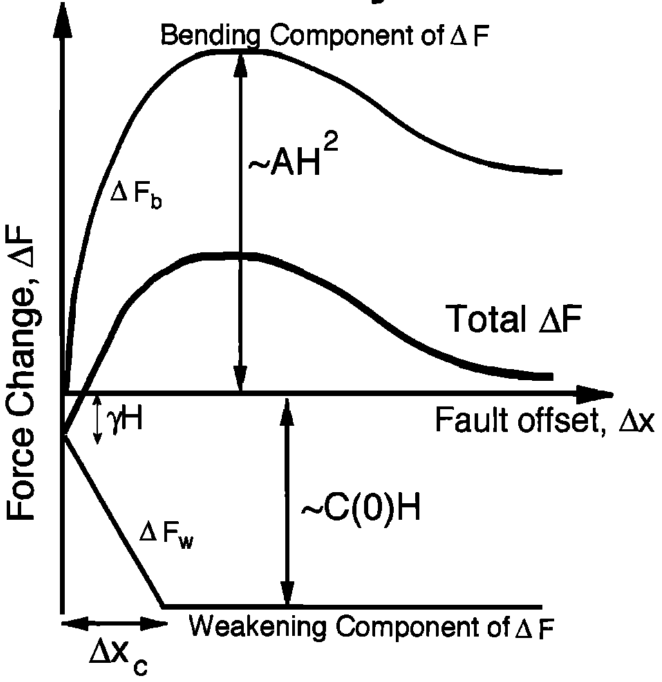
\includegraphics[width=0.45\textwidth]{./Figures/fig_Results_Weakening_1_tradeOff_bend_weak.png}
 \caption[Trade-off between change in bending force $\Delta F_{b}$ and weakening in the fault interface $\Delta F_{w}$. Adapted from \citep{Lavier2000}.]{Trade-off between change in bending force $\Delta F_{b}$ and weakening in the fault interface $\Delta F_{w}$. H is the thickness of the brittle crust and $\gamma$ is the size of initial weak perturbation and A defines the maximum bending force change. Adapted from \citep{Lavier2000}. (For more details, please refer to \citep{Lavier2000})}
 \label{fig_Results_Weakening_1}
\end{figure}

The parameters that controls fault alternation have been proposed by \citet{Lavier2000}. \citet{Lavier2000} focused on the trade-off between bending forces ($\Delta F_{b}$) as a function of fault offset $\Delta X$ and force change due to strain weakening ($\Delta F_{w}$) that is also a function of  $\Delta X$. They showed that the strength weakening on the existing fault combined with bending force resists further offset of the fault plays a major role in determining the stress state at the regions other than the active fault. Their analysis explains how higher characteristic fault slip ($\Delta X_{c}$) or slower strain weakening results in multiple faults rather than only one fault lasting. %Whether conjugate fault and even multiple faults can be produced depends on the local stress condition. 
 As $\Delta X$ increases on a fault at a spreading center, the change in bending force $\Delta F_{b}$ increases and the strength at the fault interface decreases due to weakening $\Delta F_{w}$ (Figure~\hyperref[fig_Results_Weakening_1]{\ref{fig_Results_Weakening_1}}). If the net force change $\Delta F = \Delta F_{b}+ \Delta F_{w}$ is positive, it means that it becomes harder to maintain the existing fault and stress begins to accummulate at other areas which eventually break another fault. $\Delta F_{b}$ initially increases fast with respect to $\Delta X$ and then when the detachment fault surface roll over, $\Delta F_{b}$ reaches its peak value and begins to decrease a little and maintains at a constant value. If the strain weakenging is fast enough that the net effect force $\Delta F$ is always negative, then most of the stress will be released by the existing fault and thus no conjugate or multiple faults will be generated. 
Our model results are consistent with this analysis in that only weakening (slower weakening with higher $\Delta X_{c}$) produces an alternating normal fault on the conjugate plate.

%Based on the previous experience in pseudo-2D models and \citep{Lavier2000},  when M$>0.5$, the frequency of normal faulting alternation is higher for higher characteristic fault offset ($\Delta X_{c}$) of Type two weakening compared to Type one weakening. However, for the reference model two, M88ConT2 (Table~\hyperref[Tab1_1]{\ref{Tab1_1}}), interesting enough, when comparing pseudo-2D and 3D models with Type two weakening under case of M$=0.8$, even though the 3D Model has a larger $\Delta X_{c}$ of 1km than that of pseudo-2D model of 0.5kmr, the 3D model M88ConT2 has a lower frequency of faulting alternation. Since M is constant 0.8 along the ridge-axis, the effect of along ridge couplingthat resists alternation need not be considered. One possibility is that the resisting bending force increase in a higher rate than linear with respect to increasing the length of the ridge segment (Z$_{max}$ km).  

\subsubsection{Mass wasting}

\begin{figure}[h]
 \centering
  \includegraphics[width=1.0\textwidth]{./Figures/fig_Discussion_Observation_1_13N_MAR_CutBack.eps}
 \caption[Comparing bathymetry at 13$\degree$N Mid-Atlantic Ridge to the mass wasting behavior of M28SqrtT1.]{Comparing bathymetry at 13$\degree$N Mid-Atlantic Ridge to the mass wasting behavior of M28SqrtT1. The model topography is a mirror symetric flip according to the dash line, it shows the case of M varies in a square root functional form from 0.2 to 0.8 to 0.2. The bathymetry image is generated by GeoMapApp \citep{Ryan2009}.}
 \label{fig_Discussion_Observation_1_13N_MAR_CutBack}
\end{figure}

\begin{figure}[h]
 \centering
  \includegraphics[width=0.8\textwidth]{./Figures/fig_Discussion_Observation_3_MassWasting_13-15N_bathymetry_magnetizaion.eps}
 \caption{Bathymetry and magnetization of 13$\sim$15 $\degree$N MAR. Adapted from \citep{Smith2008}.}
 \label{fig_Discussion_Observation_3_MassWasting_13-15N_bathymetry_magnetizaion}
\end{figure}

The mass wasting behavior in M28SqrtT1 model produces a fault scarp of $\sim$1km in relief, 40km in length along isochron-parallel direction. It seems to form when the detachment fault rolls over and induces bending stressses that generate the high angle fault which cuts the weak detachment fault surface and decouples the spreading breakaway and the highly deformed fault hanging wall. The topography at 13$\degree$N Mid-Atlantic Ridge also has a fault scarp with very similar curved geometry with $\sim$1km in relief. However, the 1 km relief might be relfecting the model resolution of 1 km so further investigation is necessaray. In addition, a magnetic anomaly study of the region from \citep{Smith2008} reveals a perfect match at the 13 $\degree$ 5 $^{\prime}$N between the bathymetry and the magnetization (Figure~\hyperref[fig_Discussion_Observation_3_MassWasting_13-15N_bathymetry_magnetizaion]{\ref{fig_Discussion_Observation_3_MassWasting_13-15N_bathymetry_magnetizaion}}). It might imply that the block at 13 $\degree$ 5 $^{\prime}$N ajacent to the curved fault scarp has a relative displacement toward the East and thus provides an evidence for the mass wasting behavior of the block.   
 
\subsubsection{Hourglass-shaped median valley}

\begin{figure}[h]
  \centering
    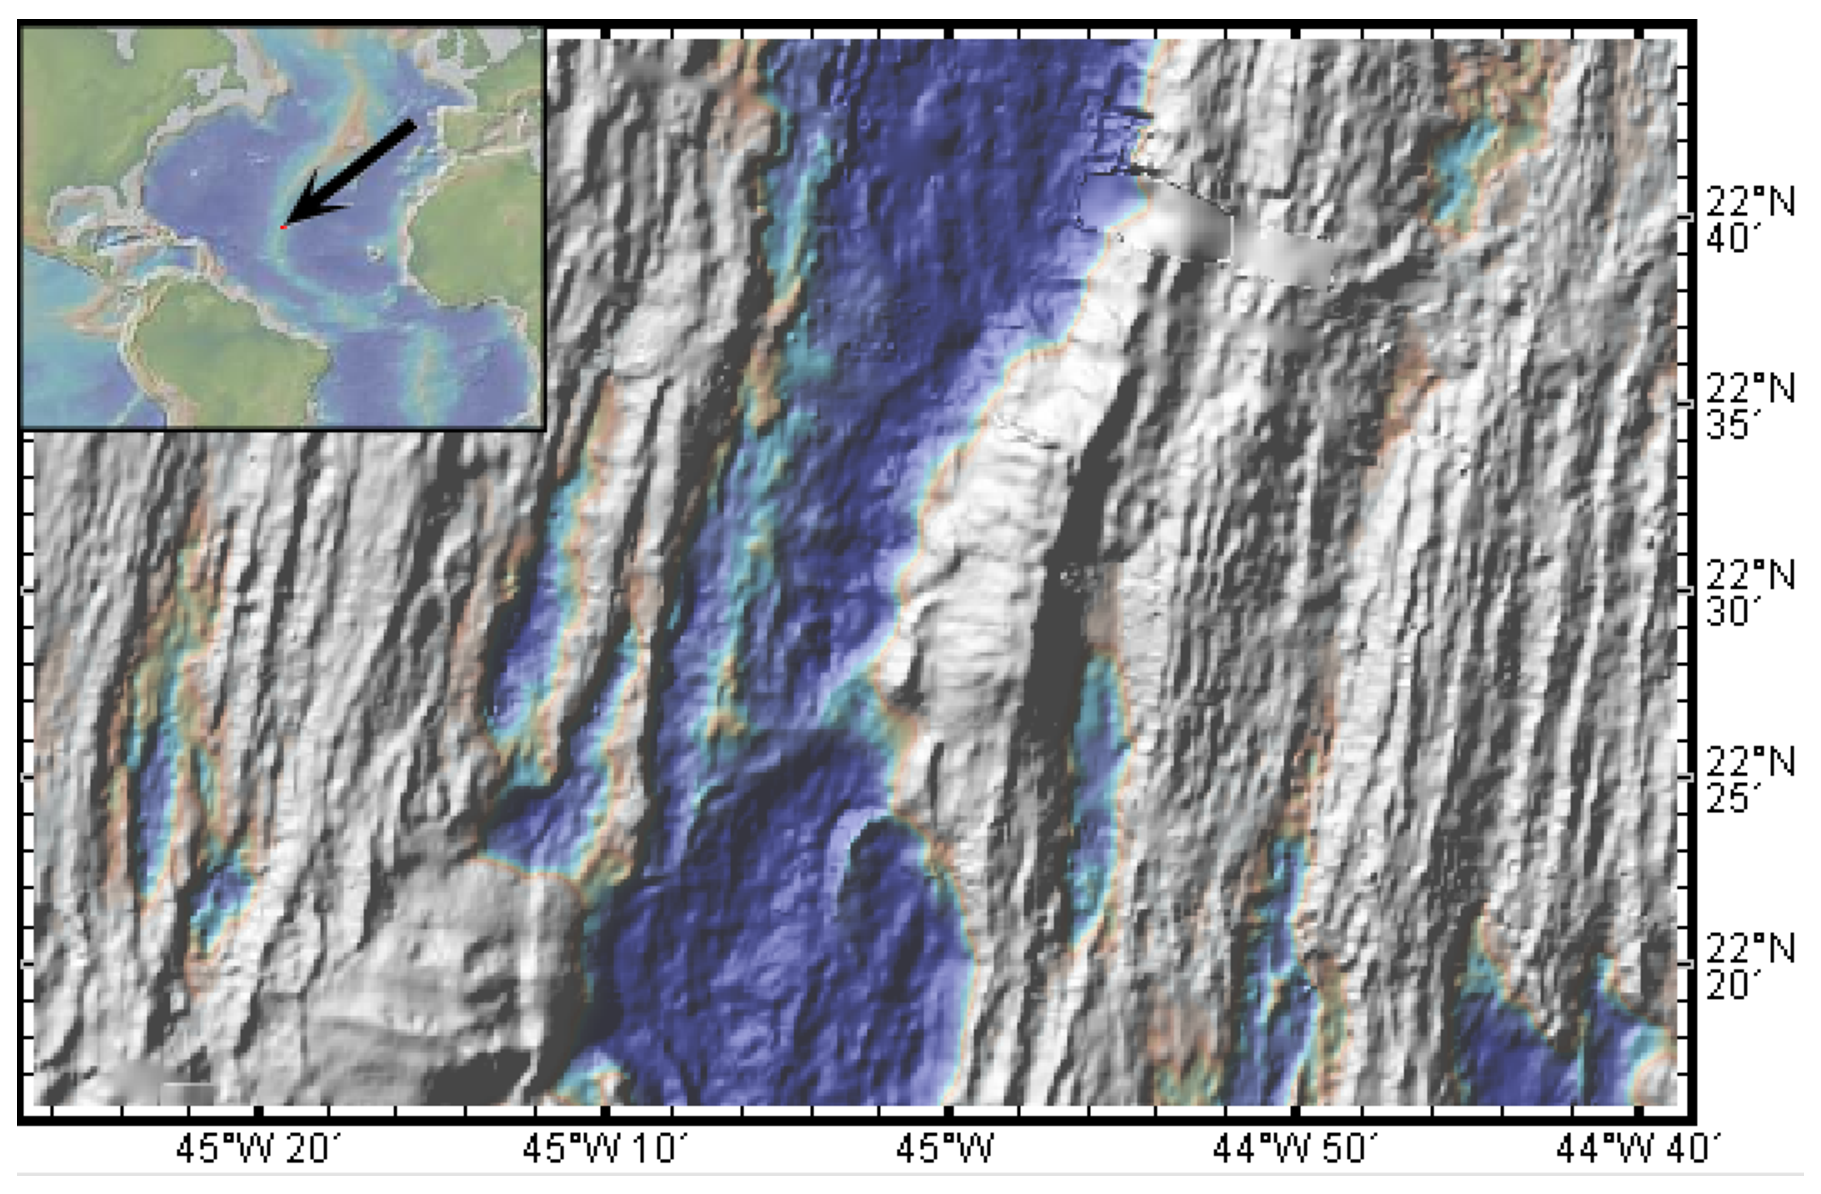
\includegraphics[width=0.5\textwidth]{./Figures/fig_Discussion_Observation_4_hourglass_22N_MAR.eps}
  \caption[Hourglass median valley at 22 $\degree$ 30 $^{\prime}$N MAR.]{Hourglass median valley at 22 $\degree$ 30 $^{\prime}$N MAR. Image is generated from GeoMapApp.}
 \label{fig_Discussion_Observation_4_hourglass_22N_MAR}
\end{figure}   

Due to the variation in diking along the ridge-axis, an hourglass shape of median valley is also produced in the model where the narrowest center corresponds to the region with higher magma supply (M=$0.8$). An hourglass-shaped median valley is frequently observed in the nature along the slow-to-intermediate spreading ridges like the Mid-Atlantic Ridges \citep{Sempere1993}, where the waist of the hourglass is usually narrower and shallower. From an analysis of the sea beam bathymetry along the MAR between 24 $\degree$ 00 $^{\prime}$N and 30 $\degree$ 40 $^{\prime}$N \citep{Sempere1993}, nine hourglass shape valleys are identified. They share similar dimensional scale ($\sim$40 km $\times$ $\sim$40 km) with our model. For example, there is an hourglass around 22 $\degree$ 30 $^{\prime}$ that is 45 km long and 15 km wide (Figure~\hyperref[fig_Discussion_Observation_4_hourglass_22N_MAR]{\ref{fig_Discussion_Observation_4_hourglass_22N_MAR}}). The observed width and depth of the hourglass can be used for inferring which evolution stage the rift valley is in. For instance, the one shown in Figure~\hyperref[fig_Discussion_Observation_4_hourglass_22N_MAR]{\ref{fig_Discussion_Observation_4_hourglass_22N_MAR}} corresponds to an early stage of our model because it has a relatively symmetrical and narrow shape (Figure~\hyperref[fig_Results_3_2_hourglass_evolution]{\ref{fig_Results_3_2_hourglass_evolution}.b}). In addition, the relatively small variation in the valley's width along the ridge is more corresponding to M57 and M58 models than the M28 models. 

\subsubsection{Mullion structure}

\begin{figure}[h]
  \centering
    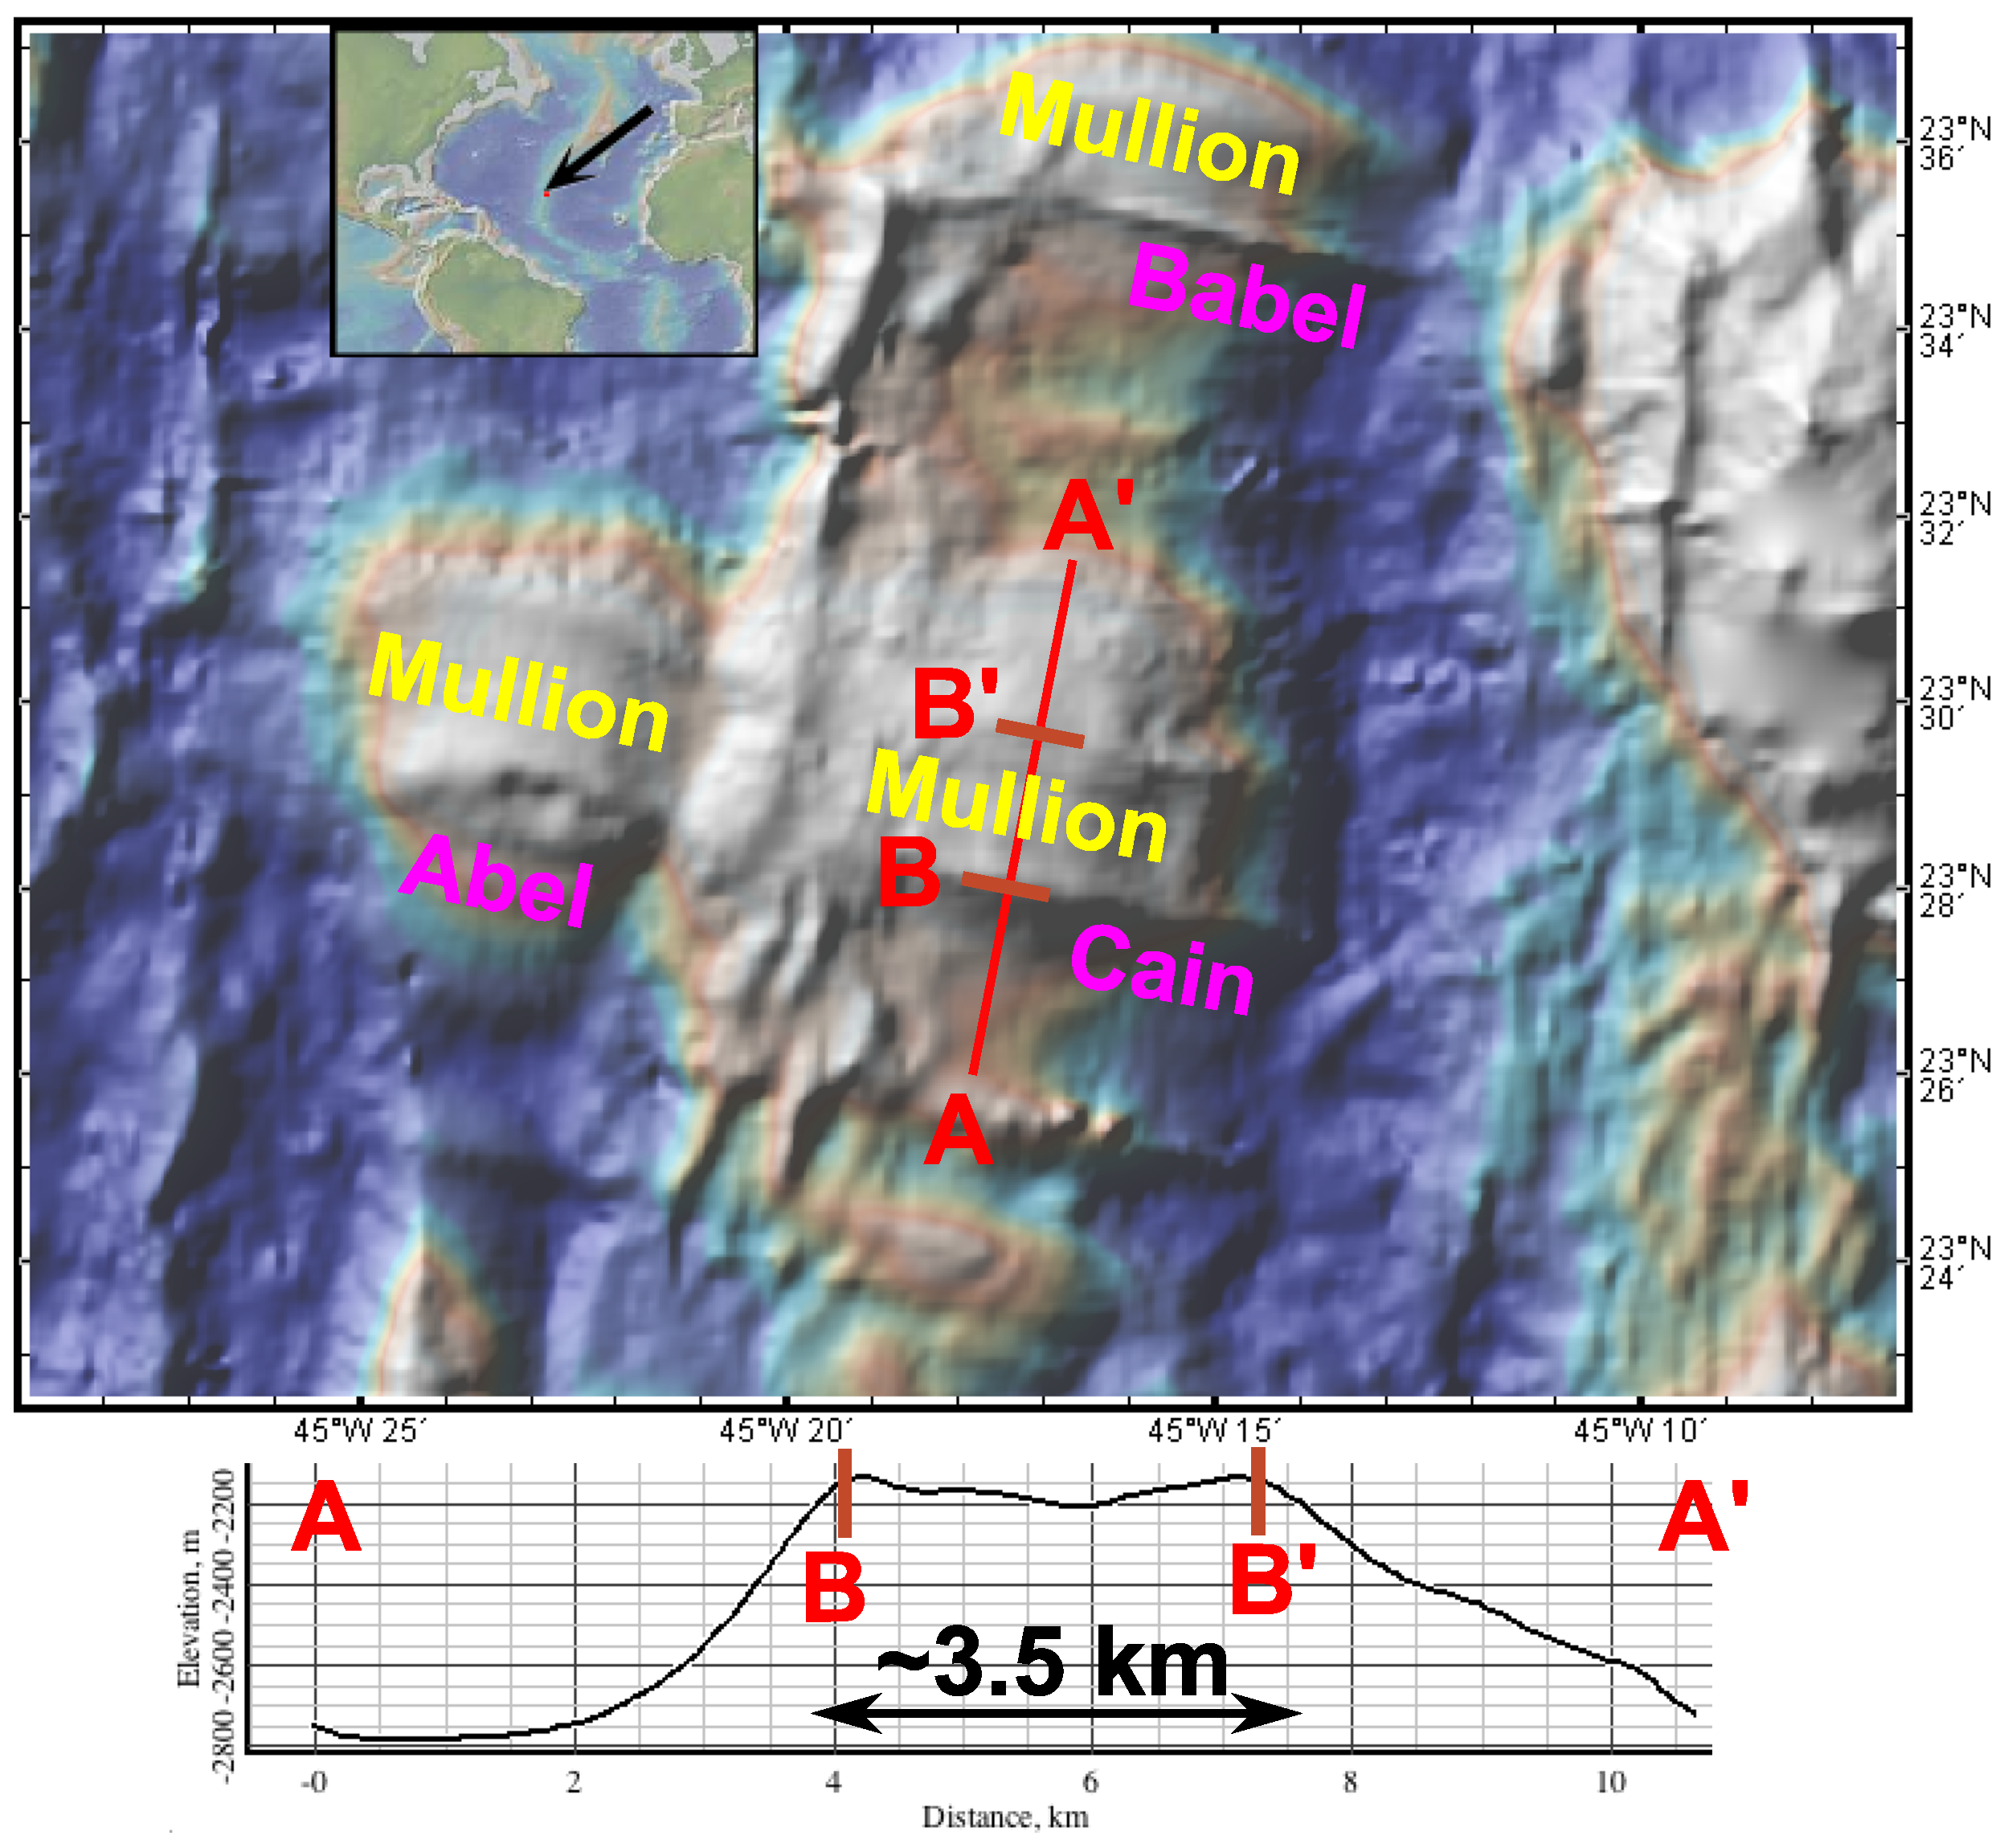
\includegraphics[width=0.8\textwidth]{./Figures/fig_Discussion_Observation_5_Mullion_Kane.eps}
  \caption[Bathymetry around the Kane OCC at 23 $\degree$N MAR.]{Bathymetry around the Kane OCC at 23 $\degree$N MAR. Image is generated from GeoMapApp.}
 \label{fig_Discussion_Observation_5_Mullion_Kane}
\end{figure}   

Mullion structures are frequently observed on the surface of OCCs. For instance, the mullion structures on the surface of of the Cain dome has a wavelength of $\sim$3.5 km as marked in the Figure~\hyperref[fig_Discussion_Observation_5_Mullion_Kane]{\ref{fig_Discussion_Observation_5_Mullion_Kane}.B$\sim$B$^\prime$}. The geometry and length scale of these mullion structures bears significant visual similarity with those of our reference model, M28LinT1 (Figure~\hyperref[fig_Results_3_2_6_mullion_evolution]{\ref{fig_Results_3_2_6_mullion_evolution}}). Model results indicate that the mullion structure mostly forms when the termination has a curved shape that can last for a long period of time and the spreading-parallel mullion structure is produced following the shape of the termination. Where the termination is curved toward the ridge axis corresponds to the larger and higher part of the mullion structure. As shown in Figure~\hyperref[fig_Discussion_Observation_2_Dick2008_Kane]{\ref{fig_Discussion_Observation_2_Dick2008_Kane}}, the spatial distribution of the mullion structure of the Cain dome is consistent with the termination that is curved inward to the ridge axis.

\subsubsection{Corrugations}

\begin{figure}[h]
  \centering
    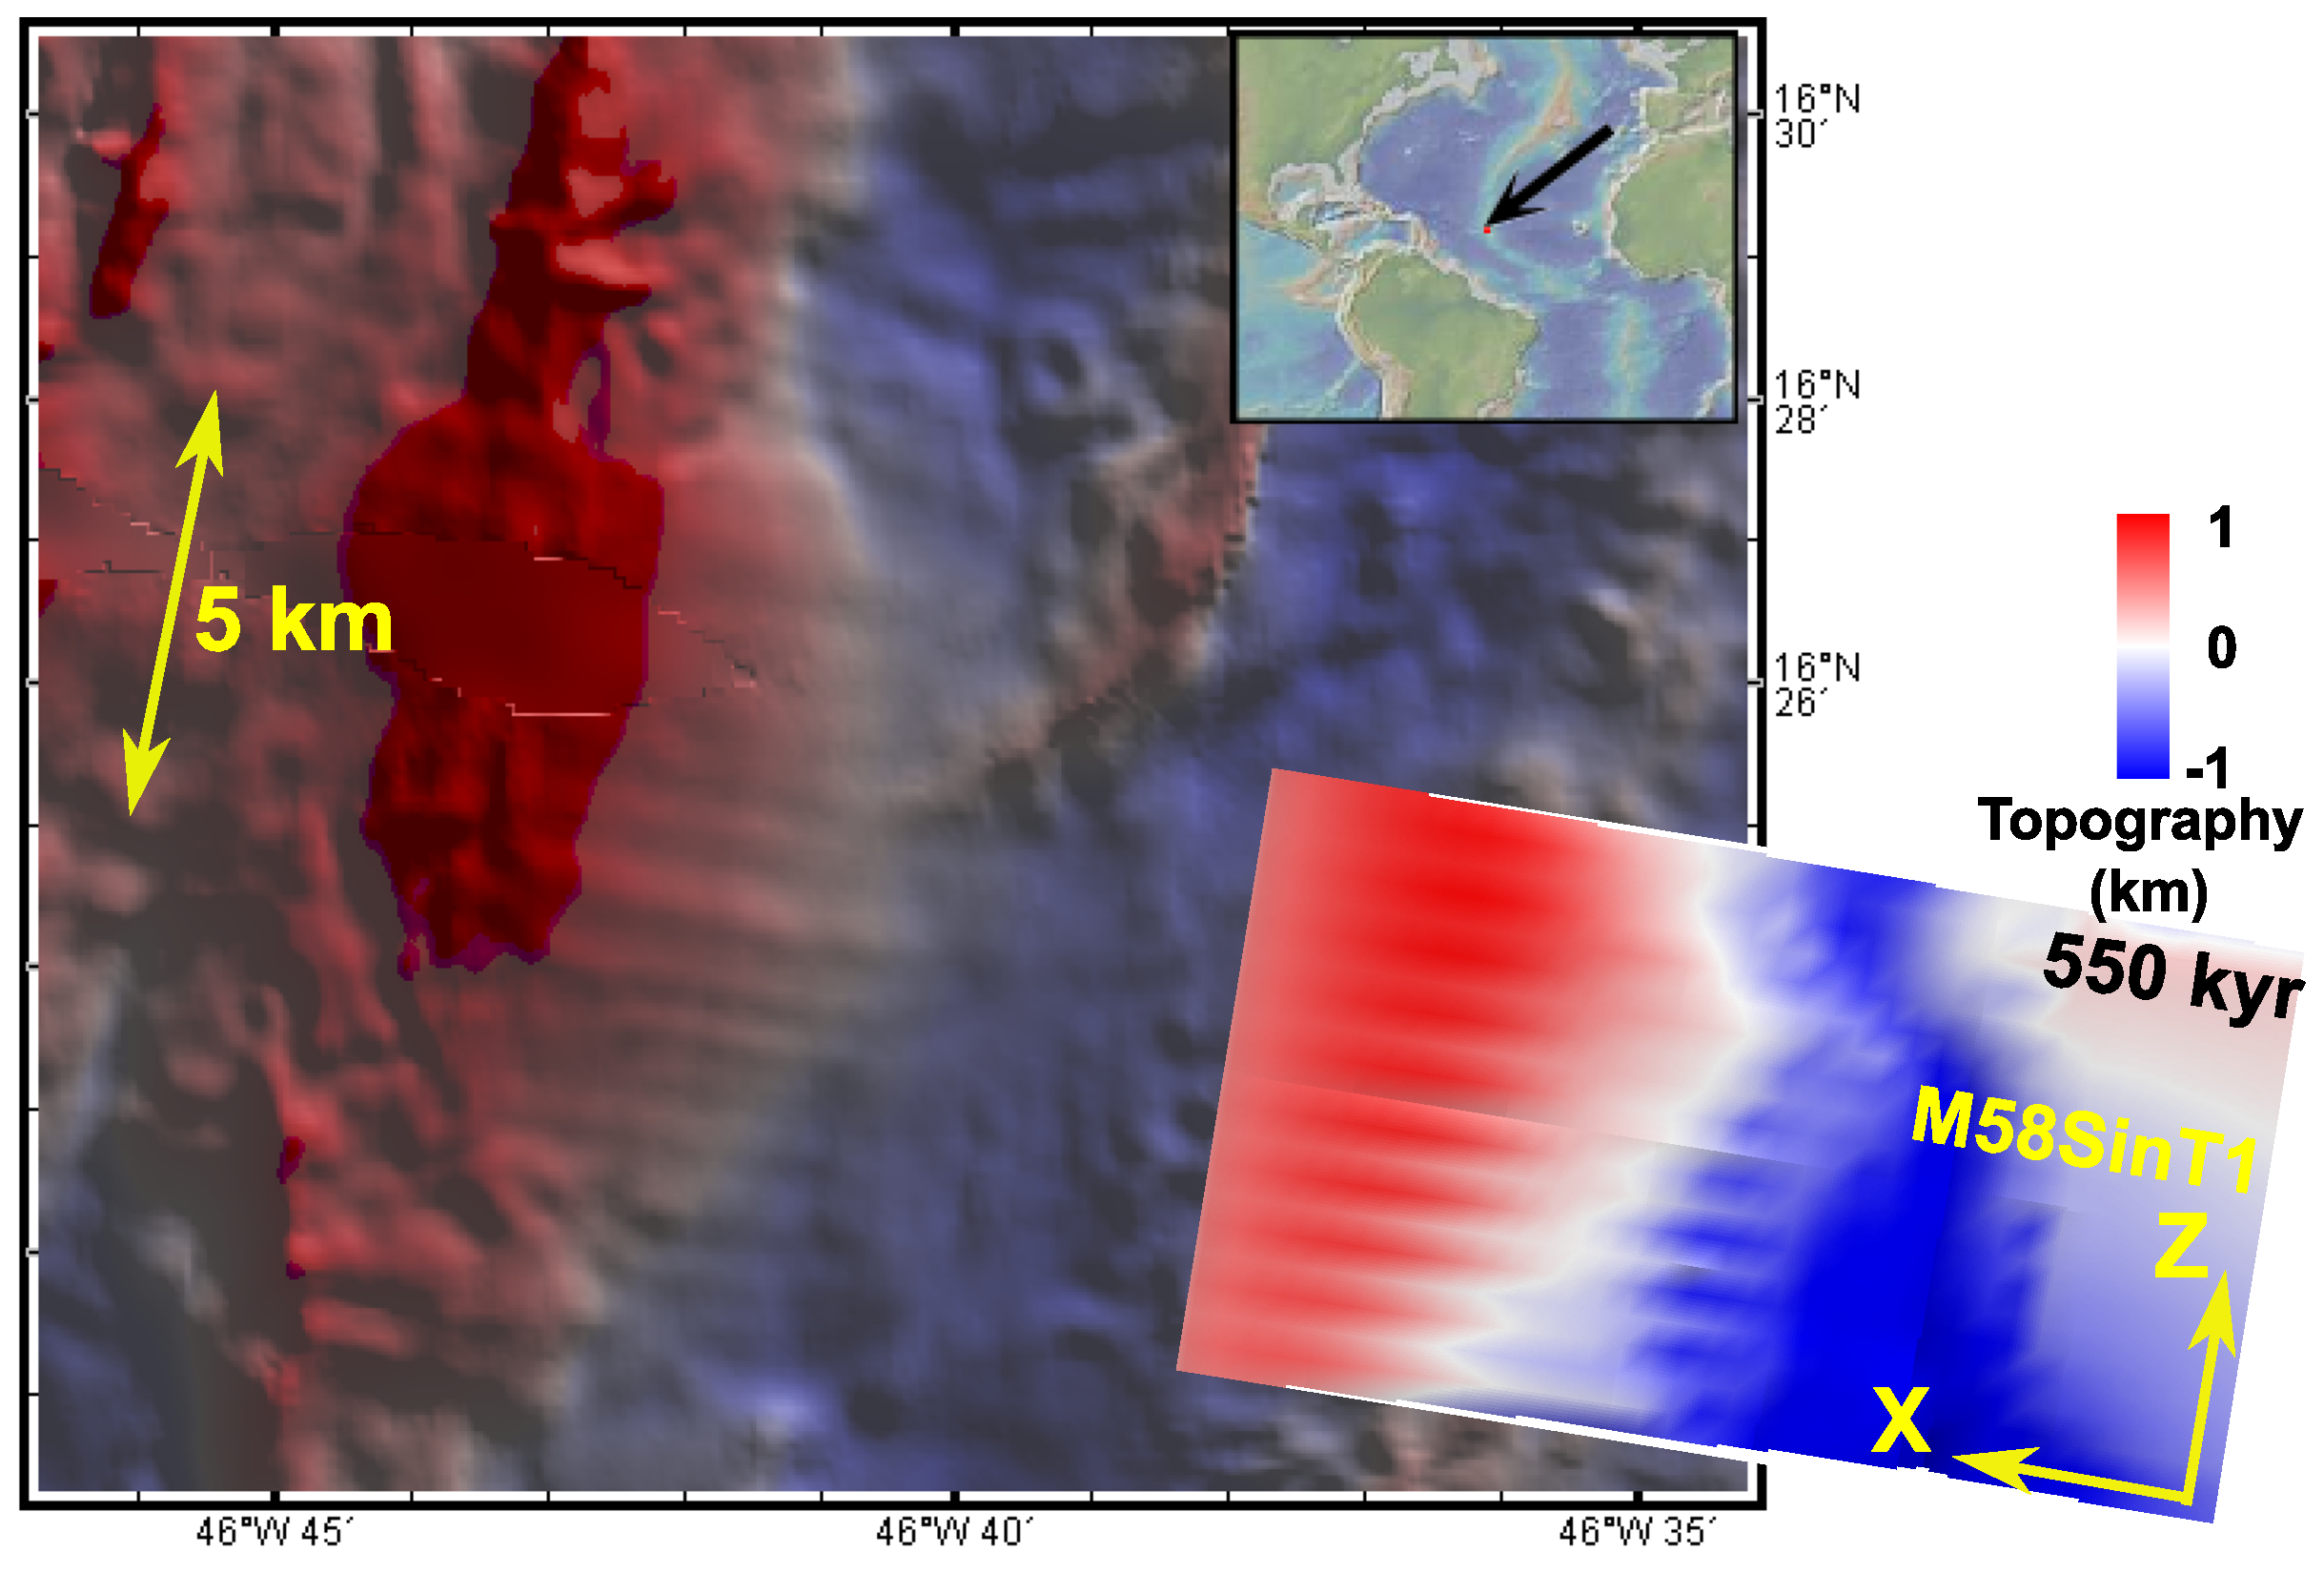
\includegraphics[width=0.8\textwidth]{./Figures/TOBE_USED_fig_Discussion_Observation_Corrugations_16N_MAR.eps}
  \caption{Comparing bathymetry at 16 $\degree$N Mid-Atlantic Ridge to the corrugations of M58SinT1 at 550 kyr.}
 \label{fig_Discussion_Observation_Corrugations16N_M58SinT1}
\end{figure}

Observed corrugations are also produced in the models. For instance, the spreading-parallel corrugations with wavelength of several kilometers that appear on the surface of the OCC at 16 $\degree$N Mid-Atlantic Ridge are reproduced by model M58SinT1 (Figure~\hyperref[fig_Discussion_Observation_Corrugations16N_M58SinT1]{\ref{fig_Discussion_Observation_Corrugations16N_M58SinT1}}).

\begin{figure}[h]
  \centering
    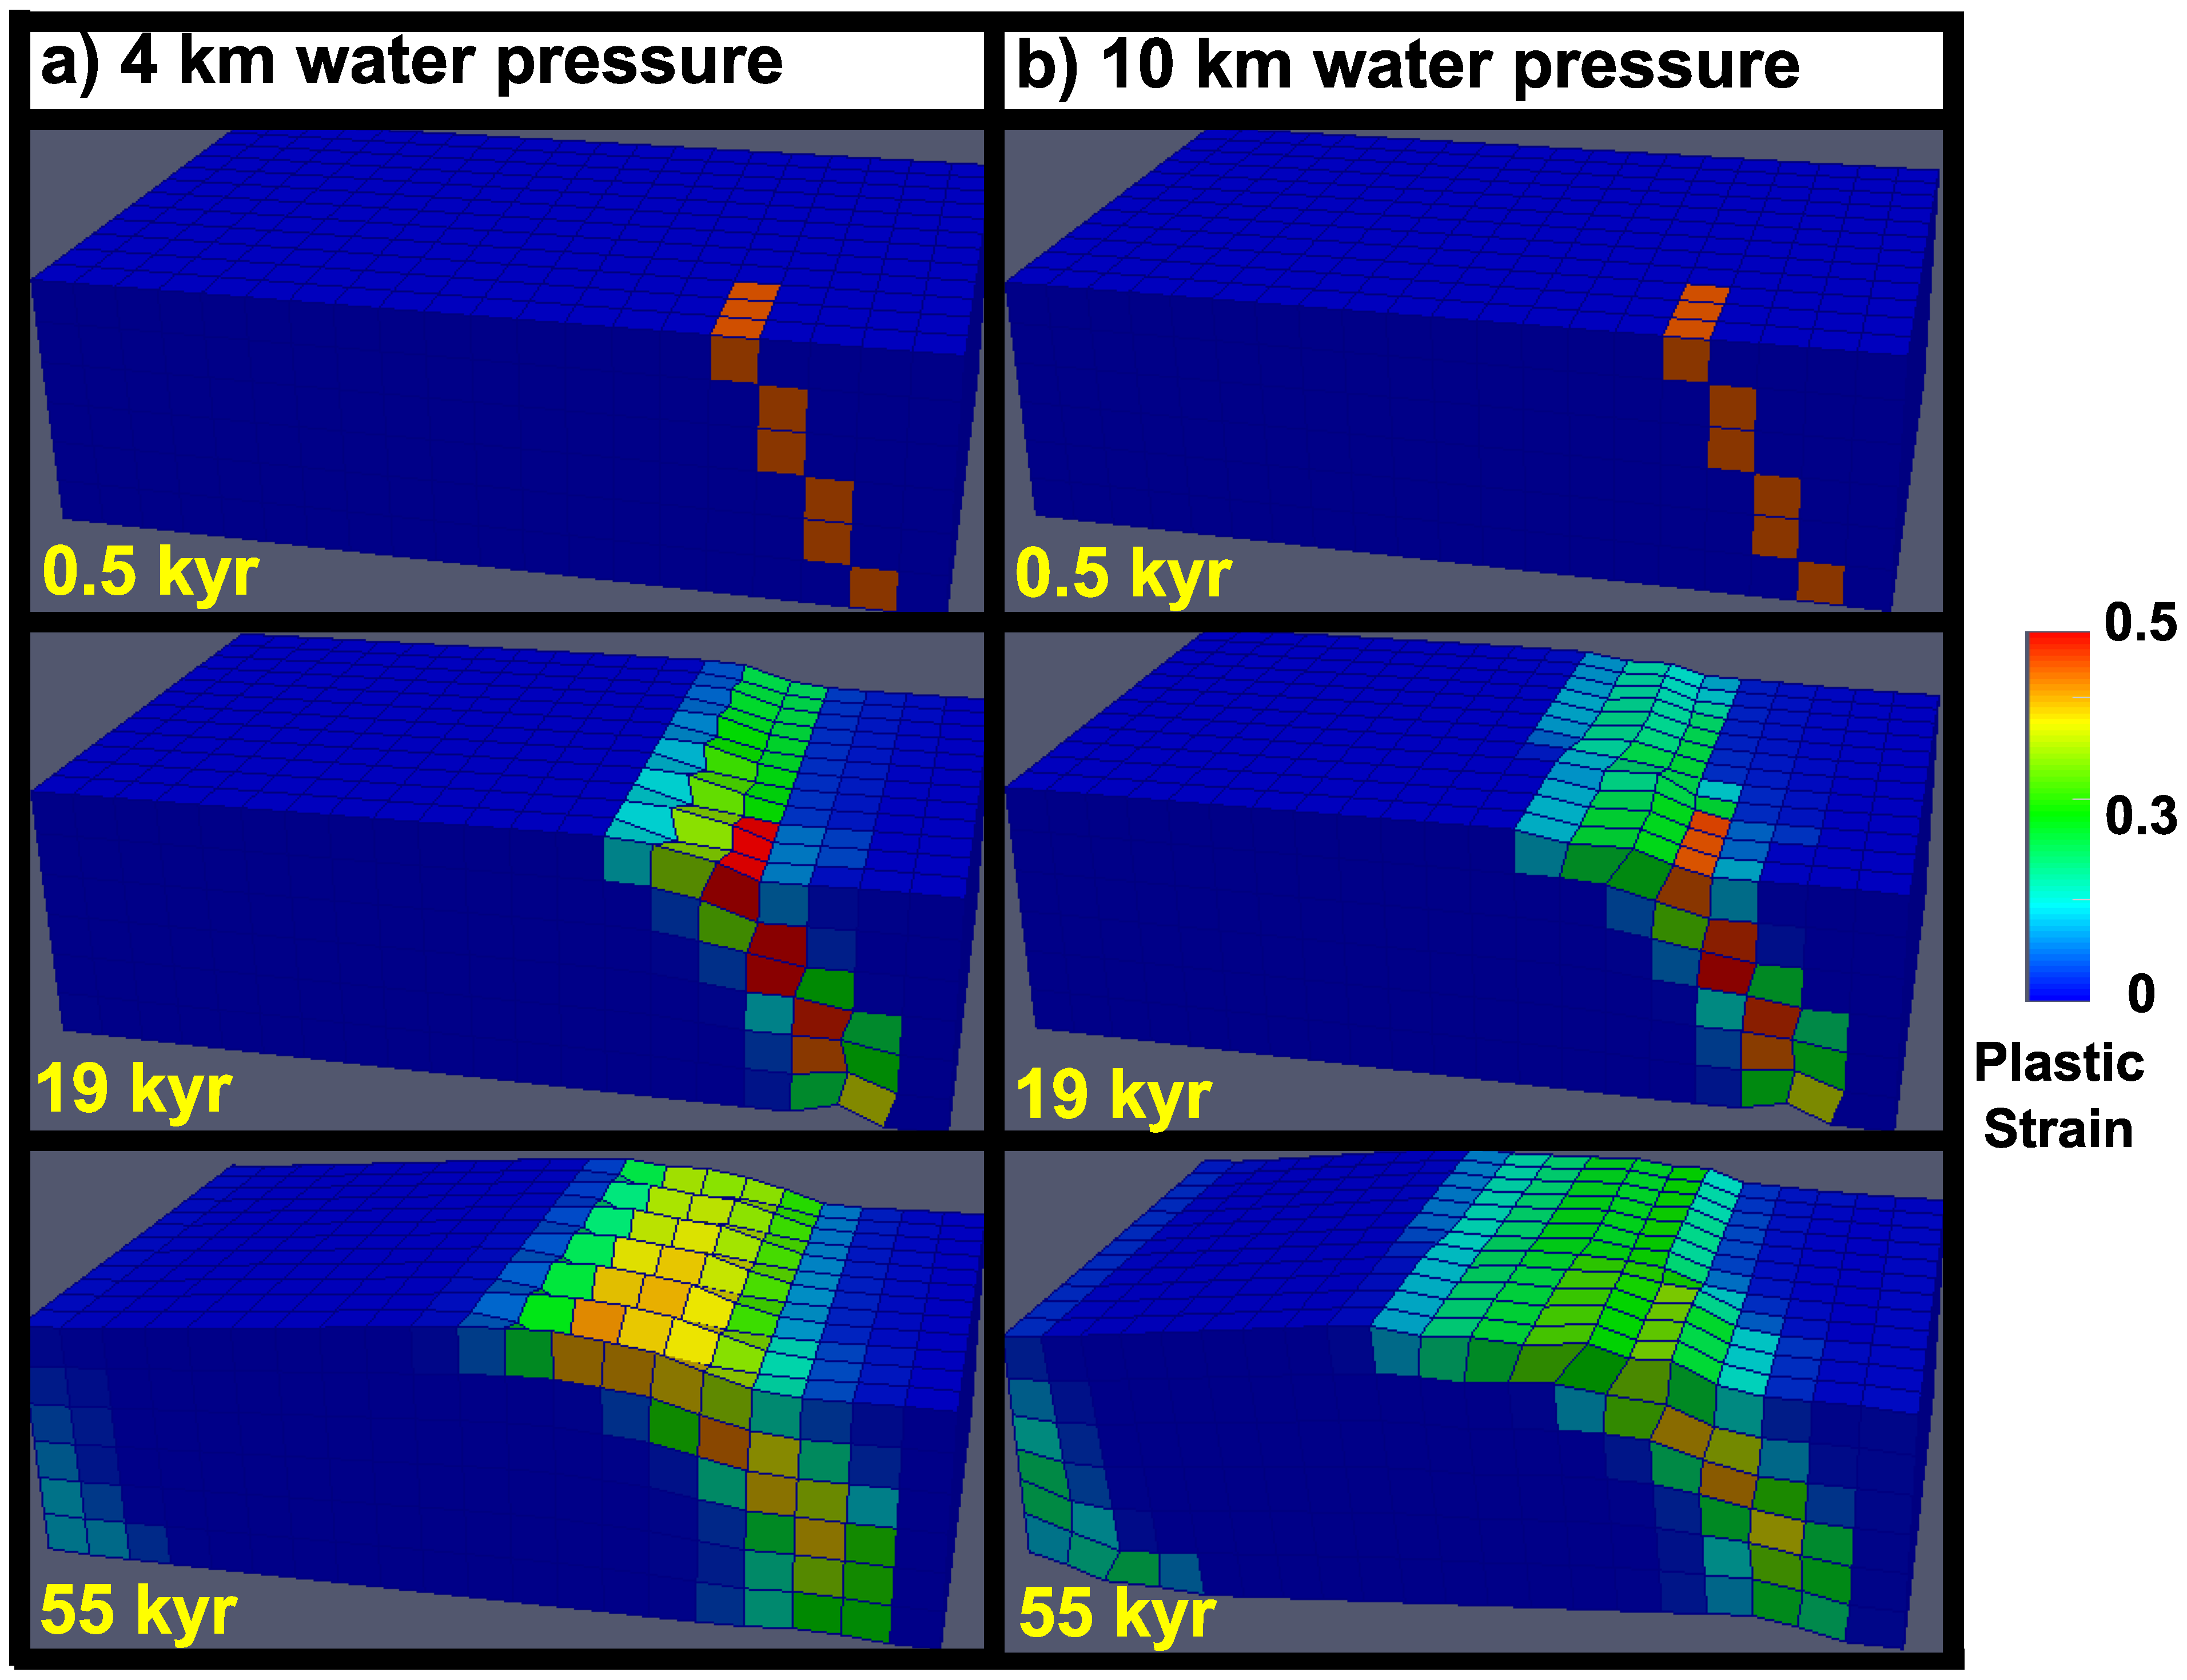
\includegraphics[width=0.8\textwidth]{./Figures/fig_Discussion_simple_models_for_corrugation_mechanism.eps}
  \caption[Simpler 3D models for formation mechanism of corrugation.]{a) Plastic strain evolution of simpler 3D model with 4 km of seawater pressure on top; b) Plastic strain evolution of simpler 3D model with 10 km of seawater pressure on top. Seeds (elements with initial plastic strain) are partially added along the ridge segment.}
 \label{fig_Discussion_simple_models_for_corrugation_mechanism}
\end{figure}

\begin{figure}[h]
  \centering
    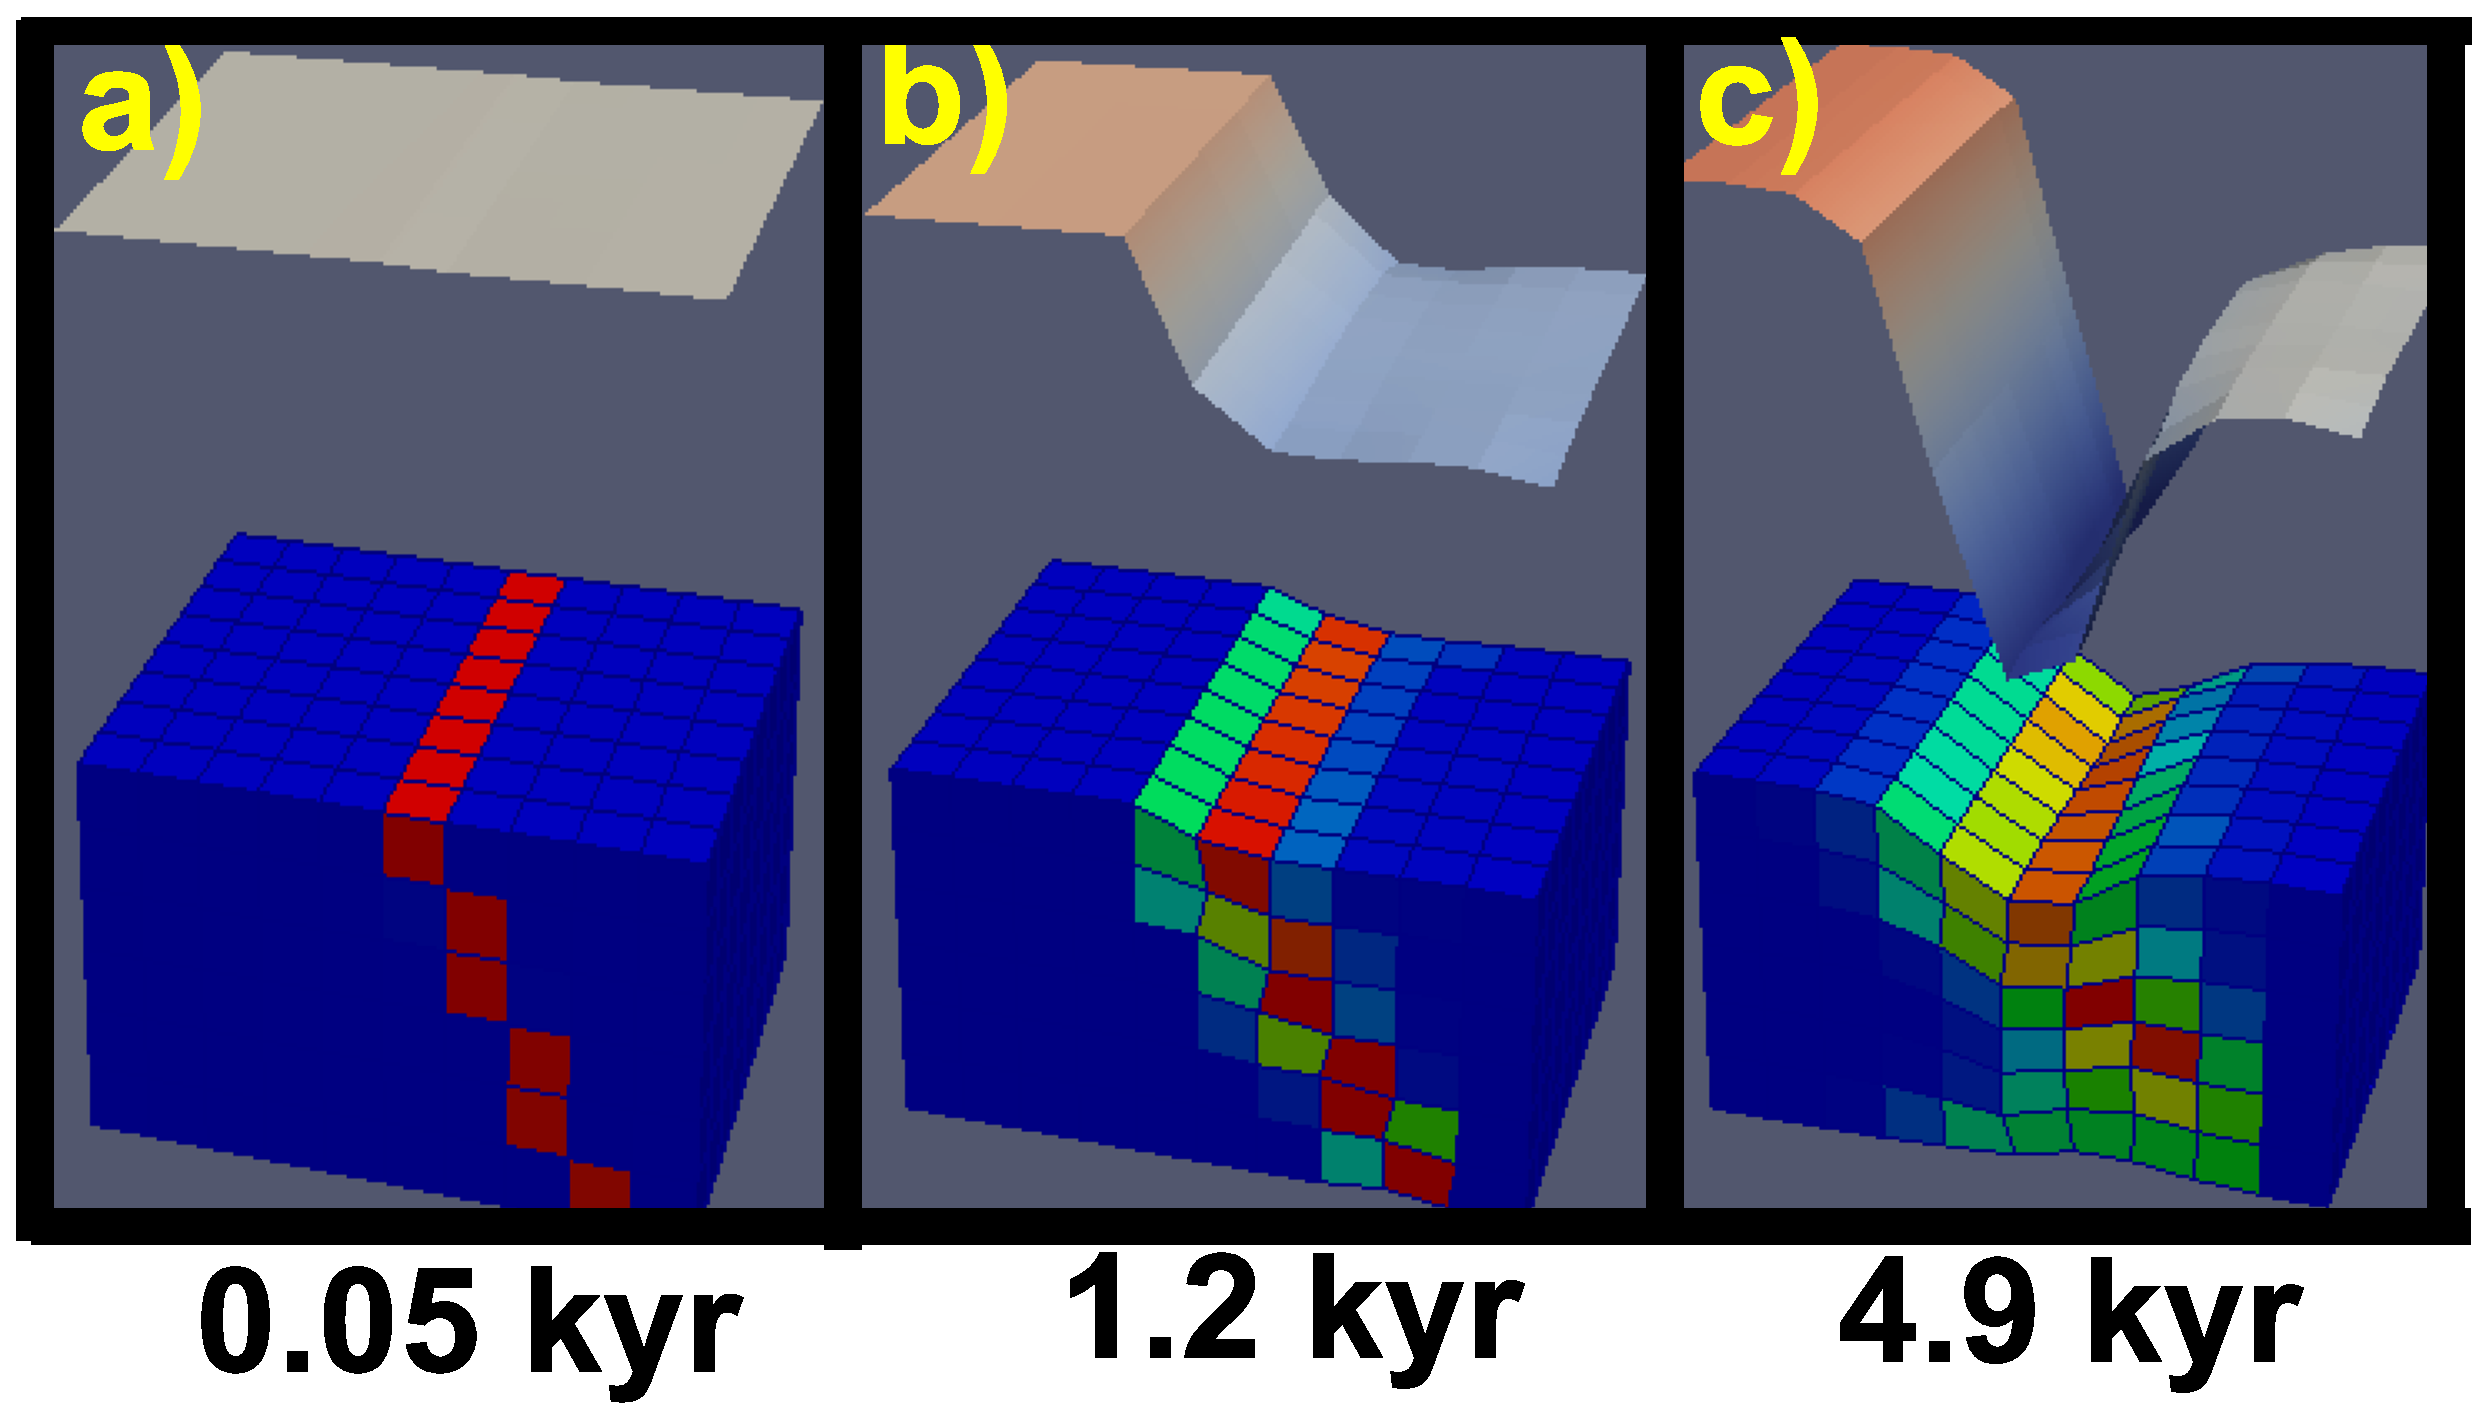
\includegraphics[width=0.6\textwidth]{./Figures/fig_Discussion_Observation_6_Corrugation_simplerModel_4kwaterdepth_along_ridge_seed.eps}
  \caption[Simpler 3D model with 4 km of seawater pressure on top. Seeds are added along the whole ridge segment.]{Simpler 3D model with 4 km of seawater pressure on top. Seeds are added along the whole ridge segment. Color scale is the same as Figure~\hyperref[fig_Results_3_2_6_corrugations_evolution]{\ref{fig_Results_3_2_6_corrugations_evolution}}.}
 \label{fig_Discussion_Observation_6_Corrugation_simplerModel_4kwaterdepth_along_ridge_seed}
\end{figure}   

As decribed in the ``Results'' section, the corrugations are formed due to the moving off axis tensile failure which results from the asynchronous faulting along the ridge. This mechanism is further verified by simpler 3D models.

When seeds (elements with prescribed plastic strain of 0.5) are partially added along the ridge segment for simulating the effects of asynchronous faulting where normal fault initiates earlier at the region with initial seeds, corrugations are produced by the model (Figure~\hyperref[fig_Discussion_simple_models_for_corrugation_mechanism]{\ref{fig_Discussion_simple_models_for_corrugation_mechanism}.a}). 
However, when 10 km of sea water pressure is added on top of the seafloor to suppress tensile failure, no corrugation is produced (Figure~\hyperref[fig_Discussion_simple_models_for_corrugation_mechanism]{\ref{fig_Discussion_simple_models_for_corrugation_mechanism}.b}). This verifies that the corrugation is related to tensile failure at the exposed fault plane.

In addition, when seeds are added along the whole ridge segment, which results in synchronous faulting, no corrugation is generated (Figure~\hyperref[fig_Discussion_Observation_6_Corrugation_simplerModel_4kwaterdepth_along_ridge_seed]{\ref{fig_Discussion_Observation_6_Corrugation_simplerModel_4kwaterdepth_along_ridge_seed}}). This verifies that along ridge asynchronous faulting induced isochron-parallel tensional stress is necessary for creating corrugations.

As mentioned in \citep{Smith2014}, wavelength of corrugations varies from meters to kilometers. Different scales corrugations sometimes coexist on the surface of a single OCC (e.g. \citealp{MacLeod2009}). Although corrugation is a widely observed phenomenon, its formation mechanism is still mysterious \citep{Smith2006}. Several hypotheses were proposed. \citet{Spencer1999} explains the corrugation by applying a continuous casting model which is analogical to the industrial casting process that the hot and ductile footwall of a detachment fault is continuously exhumed to the surface while being casted by the cold and brittle hanging wall. The domal shape of the corrugation is produced following the shape of the hanging wall. This hypothesis is similar to the formation mechanism of the mullion structure produced in our models. \citet{Smith2014} proposes another hypothesis that pre-existing offsetted faults along the ridge break through and connect to each other and form a curved termination that can produce corrugations. This is called the anastomosing behavior (e.g. \citealp{Ferrill1999}; \citealp{Wong2008}) and is also produced in our models especially when there is inward fault jumps, antithetic faults or tensile failures happening at only part of the ridge segment which perturbs the continuity of the termination along the ridge. In addition, \citet{Tucholke1998} mentioned that %with respect to the tectonic configuration at mid-ocean ridges, 
as oceanic lithosphere moves off axis, horizontally isochron-parallel extension is possible due to the contraction of the cooling lithosphere.

Besides these hypotheses, I proposed that the asynchronous faulting induced tensile failure due to the varying M along the ridge axis as another possible formation mechanism for the relatively uniform $\sim$2 km corrugations. These corrugations can also be superimposed onto the surfaces of mullion structures or OCCs.

\iffalse
\subsection{Parallel computing efficiency}
\subsection{Influence of healing}
\subsection{Model Limitation}
\subsubsection{Fixed thermal structure effects and justification}
Thermal conduction rate for $\kappa=6mm^{2}/s$ material is 1.8e5 km/Myr, four magnitude faster compared to spreading rate of 2.5km/Myr.
\subsection{Recommendation for Future Research}
\fi

\iffalse
\subsection{Cut Back}\label{Sec_CutBack}

\begin{figure}[h]
  \centering
    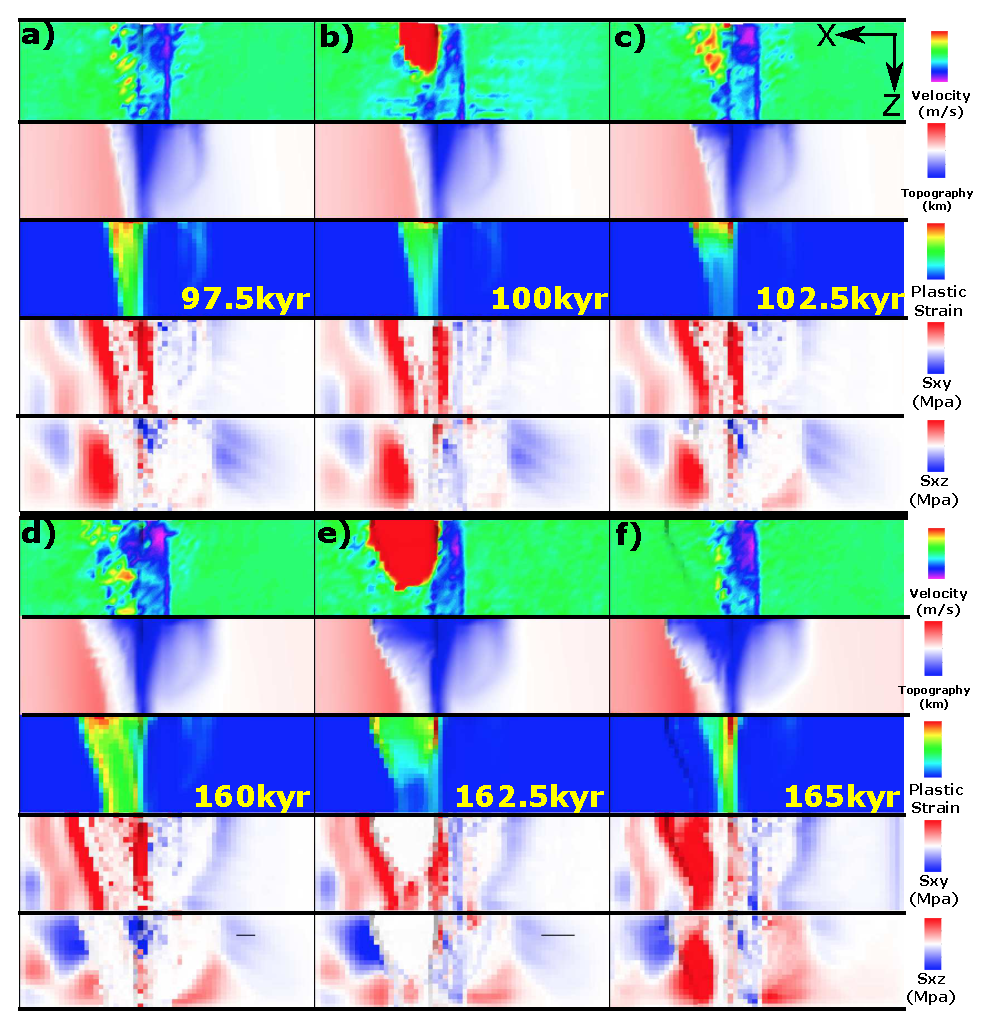
\includegraphics[width=0.8\textwidth]{./Figures/fig_Results4_4_sqrt_cut_back_with_time.eps}
  \caption{M28SqrtT1 (Table~\hyperref[Tab1_1]{\ref{Tab1_1}}). Cut back behaviors in square root functional form model with different time.}
 \label{fig_Results4_4}
\end{figure}   

\begin{figure}[h]
  \centering
    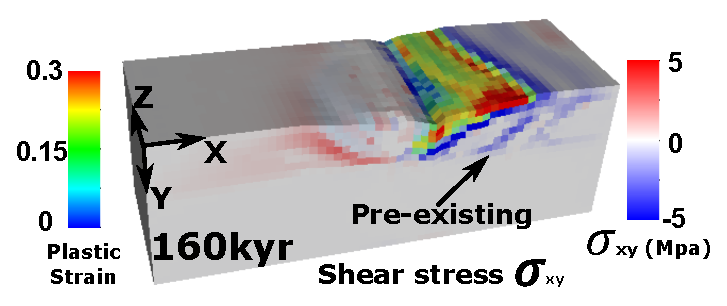
\includegraphics[width=0.6\textwidth]{./Figures/fig_Results4_5_sqrt_cut_back_pre_accummulated_shear_zone.eps}
  \caption{M28SqrtT1 (Table~\hyperref[Tab1_1]{\ref{Tab1_1}}). Square root functional form model at 160kyr. Pre-accummulated shear zone increase the shear force and cut the weak detachment front tip}
 \label{fig_Results4_5}
\end{figure}   

The cut back happens mostly in the square root model. Since the linear model and the square root model have more obvious difference in terms of the cut back behavior, here, we only compare linear and square root. There are several factors contribute to the cut back behavior. First, at the higher M side, the amount of diking for the square root model is ubiquitously larger than that of the linear one (Figure~\hyperref[fig_Results3_1]{\ref{fig_Results3_1}}). This leads to a slower bending detachment at the high M side for the square root model. Second, the totoal length of the ridge segment with M$>0.5$ for the square root model is also longer than that of the linear one (Figure~\hyperref[fig_Results3_1]{\ref{fig_Results3_1}}). This results in that at the low M side, $\sigma_{xz}$ is focused at low Z ajacent to the ridge-axis (Figure~\hyperref[fig_Results4_3_1]{\ref{fig_Results4_3_1}.e}), however for linear is spread out to Z higher than 10. Third, due to higher value of $\frac{dM}{dZ}$ for square root when Z$<5$, the along ridge-axis shear $\sigma_{xz}$ for square root will be accummulating faster, which produces larger strike-slip force to cut the hanging wall at the low M side. Fourth, as observed in the model (Figure~\hyperref[fig_Results4_3_1]{\ref{fig_Results4_3_1}.c}), the parallel to spreading direction offset between breakaways along the ridge-axis is 4km for the square root model compared to 3km for the linear model. This causes the square root model to experience bigger shear stress $\sigma_{xy}$ both immediately beneath and above the fault interface at the low M side (Figure~\hyperref[fig_Results4_3_1]{\ref{fig_Results4_3_1}.d}). Fifth, as shown in Figure~\hyperref[fig_Results4_8]{\ref{fig_Results4_8}}, due to bending of the crust at the footwall side, below the blue neutral plane, $\sigma_{xx}>0$, meaning tensional stress being accummulated as fault develops. The resulting force tends to unbend the bent crust and drag down the connecting surface (the future decoupled hanging wall). All five factors together assist in the decouple of the hanging wall at the low M side as described in detail in the next paragraph.

\begin{figure}[h]
  \centering
    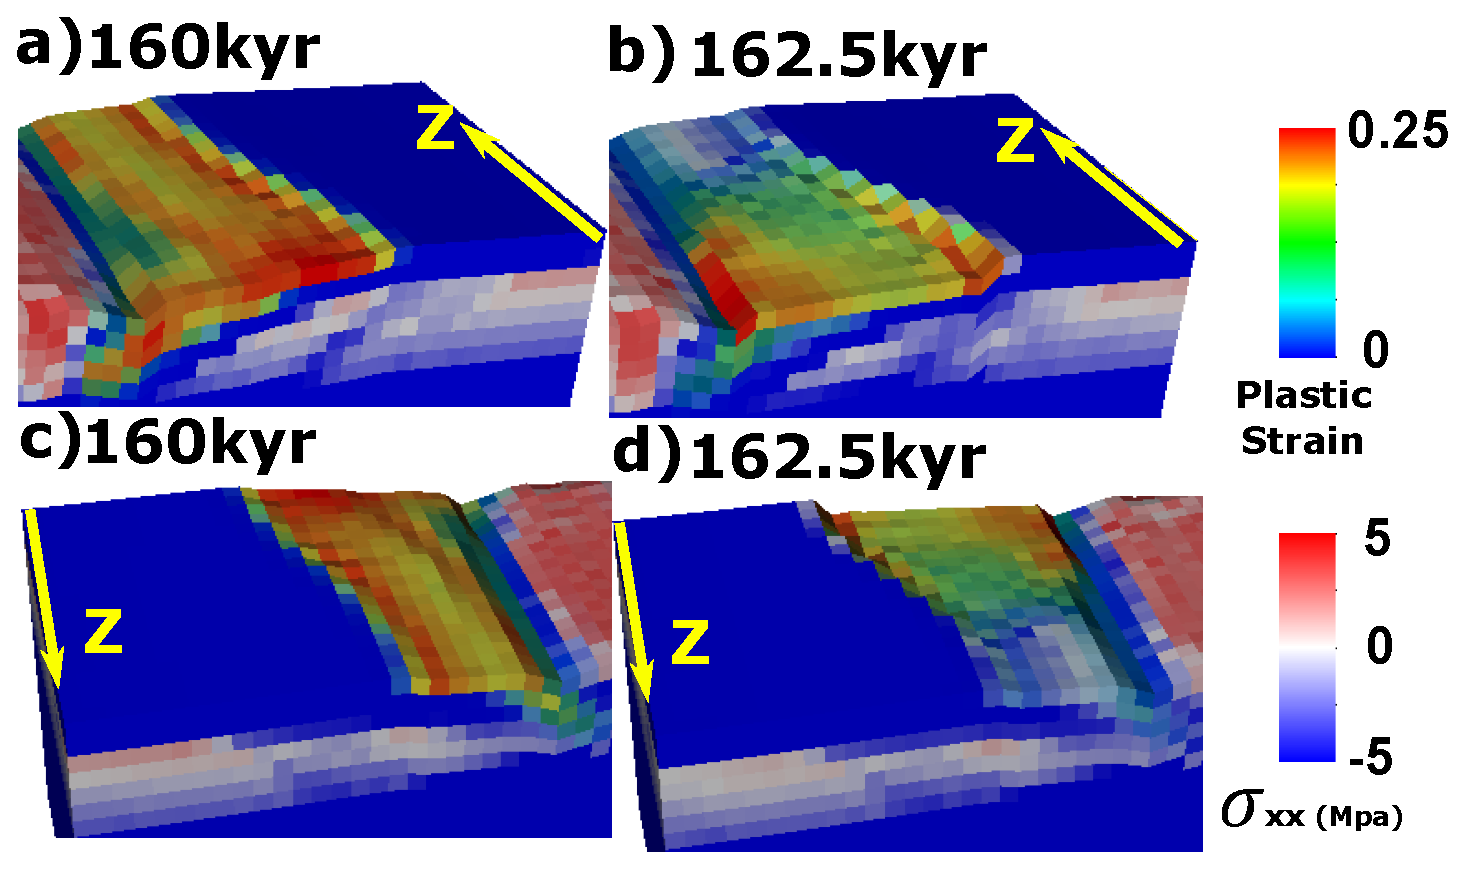
\includegraphics[width=0.6\textwidth]{./Figures/fig_Results4_6_sqrt_cut_back_bending_drop.eps}
  \caption{M28SqrtT1 (Table~\hyperref[Tab1_1]{\ref{Tab1_1}}). Bending stress drop in the crust close to dike due to cut back behavior.}
 \label{fig_Results4_6}
\end{figure}

%(Figure~\hyperref[fig_Results4_6]{\ref{fig_Results4_6}})reveals that
In the Figure~\hyperref[fig_Results4_4]{\ref{fig_Results4_4}}, the hanging wall rebounds backwards to the dike in a high velocity (Figure~\hyperref[fig_Results4_4]{\ref{fig_Results4_4}.b,e (velocity)}) accompanied with a sudden topography drop (Figure~\hyperref[fig_Results4_4]{\ref{fig_Results4_4}.b) compared to c); d) compared to e) (in the second row)}). This behavior is triggered when the front tip of the weak detachment extends further away from the ridge-axis and reaches a pre-accummulated shear zone (Figure~\hyperref[fig_Results4_5]{\ref{fig_Results4_5}}). The pre-accummulated shear zone adds extra shear force to the weak (Figure~\hyperref[fig_Results4_4]{\ref{fig_Results4_4}}.d(third row: plastic strain)) as well as shear stresses accummulated (Figure~\hyperref[fig_Results4_4]{\ref{fig_Results4_4}.d}(fourth and fifth row: $\sigma_{xy}$ and $\sigma_{xz}$)) fault interface and together with the five factors mentioned in the previous paragraph result in the cut back behavior. The cut back produces a continuous high angle fault scarp with a relief of $\sim 1km$ aligns to the initial breakaway and extends for about 20 kilometer in length (Figure~\hyperref[fig_Results4_4]{\ref{fig_Results4_4}.e (second row: topography)}). Its distance to the ridge-axis varies along the Z-axis and this result can be used to indicate the magma supply variation in the nature. \add[XT]{To be discussed in observation comparison section. as a reminder}

During the cut back process, the tensional bending stress are released at the low M side ($0<$Z$<7$) in the left tip of the bended crust (Figure~\hyperref[fig_Results4_6]{\ref{fig_Results4_6}.a compared to b}), however, in the higher M side, the tensional bending stress keeps accummulating due to the far field extension (Figure~\hyperref[fig_Results4_6]{\ref{fig_Results4_6}.c compared to d}). This behavior assists in the decouple between low M and high M side hanging walls. 

Once the cut back happens at 162.5kyr, the $\sigma_{xy}$, $\sigma_{xz}$ and $\sigma_{xx}$ are released (Figure~\hyperref[fig_Results4_4]{\ref{fig_Results4_4}.e (fourth and fifth row: $\sigma_{xy}$ and $\sigma_{xz}$)}). The plastic strain near the ridge-axis at low M side reaches a maximum of $\sim$0.9 (Figure~\hyperref[fig_Results4_4]{\ref{fig_Results4_4}.e (third row: plastic strain)}) compared to $\sim$0.3 before and after. This is due to the sudden backward motion squeezes the end element of the hanging wall near the ridge-axis and later be released by the continuous extension.

After the cut back, the termination of the detachment recedes backwards for about 7 kilometer towards the ridge-axis (Figure~\hyperref[fig_Results4_4]{\ref{fig_Results4_4}.f (third row: plastic strain)}) (termination fronts are always consistent with tension stresses in $\sigma_{xx}$ and $\sigma_{zz}$ as well as with plastic strain front(due to healing, high plastic strain region corresponds only to region with continuously deformation) (Figure~\hyperref[fig_Results4_3_1]{\ref{fig_Results4_3_1}} and Figure~\hyperref[fig_Results4_3_2]{\ref{fig_Results4_3_2}})). This behavior helps maintain a high angle normal fault. Different from the linear and sinusoidal models that the detachments at the low M side will rotate to a very low angle, square root model doesn't. In addition, $\sigma_{xy}$ and $\sigma_{xz}$ soon fill in the area between cut back created fault scarp and the new termination (Figure~\hyperref[fig_Results4_4]{\ref{fig_Results4_4}.f (fourth and fifth row: $\sigma_{xy}$ and $\sigma_{xz}$)} because $\sigma_{xy}$ always accummulates immediately beneath the normal fault interface and the red $\sigma_{xz}$ left to the new termination is due to the along ridge-axis variatioin in the rate of fault slip (low M side larger).  

\begin{figure}[h]
  \centering
    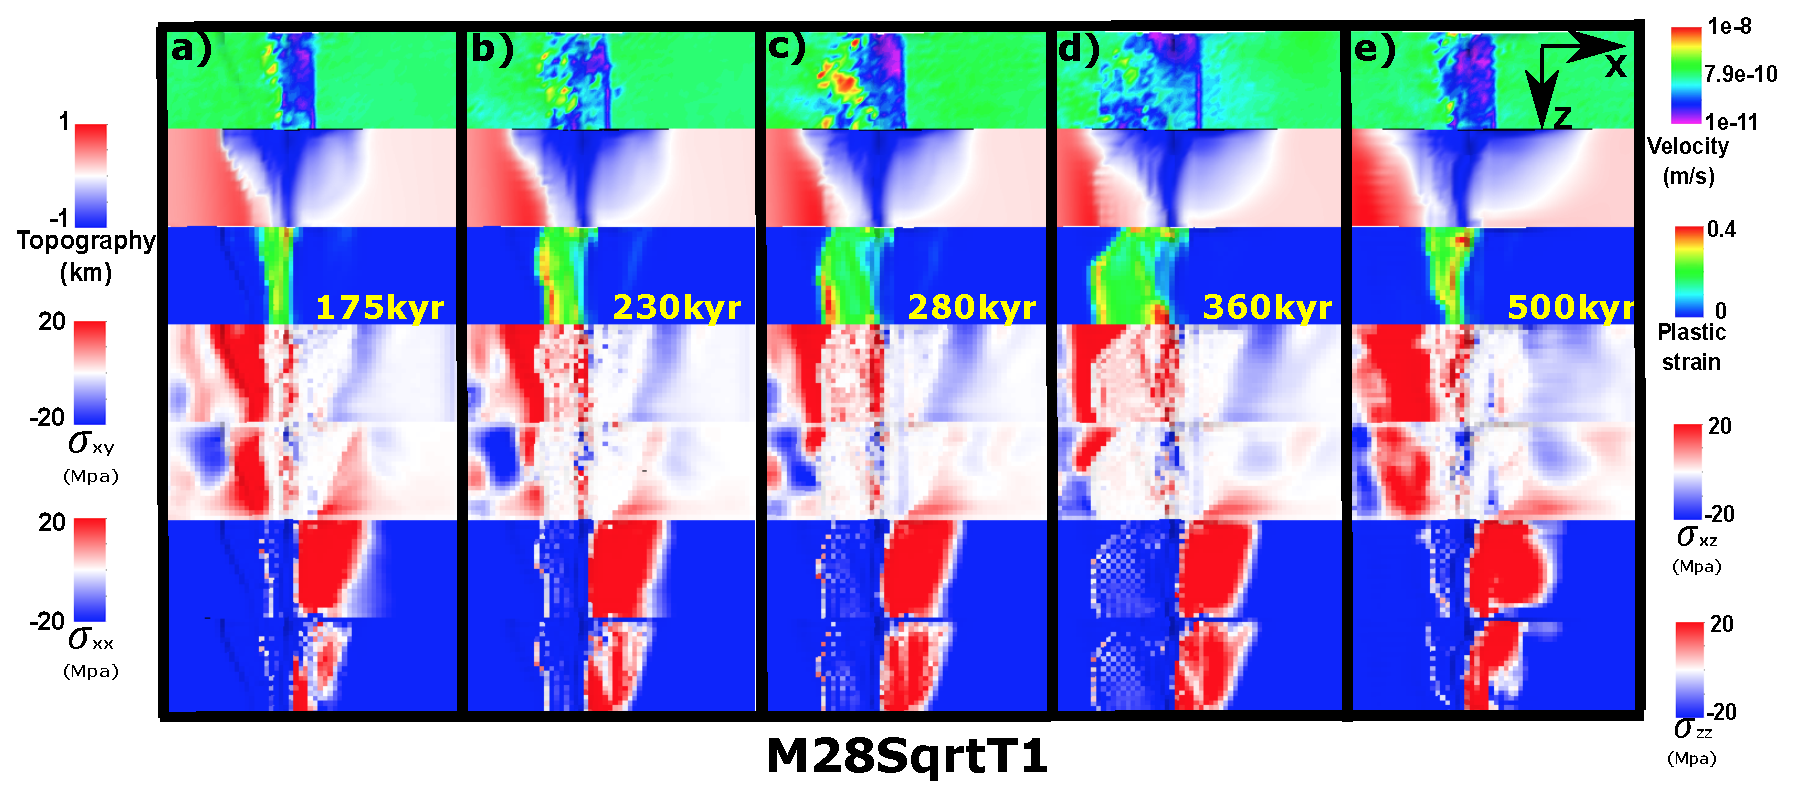
\includegraphics[width=1.0\textwidth]{./Figures/fig_Results4_9_sqrt_cut_back_new_fault_chase.eps}
  \caption{M28SqrtT1 (Table~\hyperref[Tab1_1]{\ref{Tab1_1}}). New fault front chase after initial abandoned breakaway.}
 \label{fig_Results4_9}
\end{figure}

There is one phenomenon very interesting and counter-intuitive that worth describing here. After the cut back, and termination retreat, the evolution of the detachment fronts is opposite to initiall or to the general behavior in the linear and sinusoidal models. The termination front at the high M side extends faster and further after the cut back (Figure~\hyperref[fig_Results4_9]{\ref{fig_Results4_9}}). This is partly related to the unbending decouple phenomenon we described ealier that the tensional stress are released at the low M side but continues to accummulate in the high M side during the cut back unbending in the low M side. Since the tensional stress is released in the low M side, it needs time to accummulate to where it was and then start from there to drag the new near ridge-axis fault away from the ridge-axis while at the high M side the increasing tensional stress will directly lead to a fast extending fault front. Thus create the behavior. \add[XT]{One question is, how to explain that the fault front is moving much faster than the initial abandoned breakaway? New fault front soon reach the old breakaway.} This phenomenon is largely responsible for the corrugations observed. It create a ``X'' shape ``scan'' that first ``scan'' the topography with faster low M side (Figure~\hyperref[fig_Results4_4]{\ref{fig_Results4_4}.d and e}) and then with faster high M side (Figure~\hyperref[fig_Results4_9]{\ref{fig_Results4_9}.c and d}). This results in curved terminations with hundreds to several kilometers wavelengths that directly create parallel to spreading direction corrugations.    

\begin{figure}[h]
  \centering
    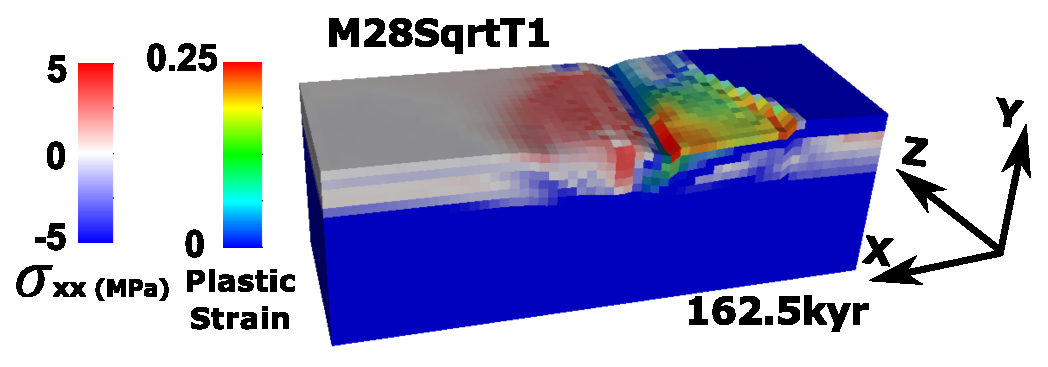
\includegraphics[width=0.6\textwidth]{./Figures/fig_Results4_7_sqrt_cut_back_conjugate_Sxx.eps}
  \caption{M28SqrtT1 (Table~\hyperref[Tab1_1]{\ref{Tab1_1}}). Higher $\sigma_{xx}$ in the median valley of conjugate plate at low M side. }
 \label{fig_Results4_7}
\end{figure}

In addition, the higher $\sigma_{xx}$ in the median valley of conjugate plate at low M side (Figure~\hyperref[fig_Results4_7]{\ref{fig_Results4_7}}) is due to the brittle crust is thinnest at the median valley, thus when same amount of force propagates from far field extension to the center median valley, the stress will increases.    
\fi



\iffalse  tables with model features
There are several behaviors that are controlled by the model parameters. Generally, only M58 models with type 2 weakening produce aternating faults on both side of the ridge axis. All the models show corrugations. As for faulting patterns in terms of evolution frequency, usually Square root is more dynamic than Sinusoidal than Linear, M58 is more dynamic than M57 than M28.

Following tables are a summery of the model behaviors with respect to different setup parameters.
 

\begin{table}[h]
\begin{small}
\begin{center}
\begin{tabular}{||l|l||l|l||l|l||}
\hline
A & Alternating Fault & C & Corrugation & SL & Shear Topography Low \\
\hline
NA& Not Alternating & SF & Secondary Fault on one side & CB & Cut Back   \\
\hline
DD &  Double Dome  & AM    & Atlantis Massif Shape &  &   \\
\hline
\end{tabular}
\end{center}
\end{small}
\caption{Model behaviors in short.}
\label{Tab1}
\end{table}

Based on the 11 models with M variation, we observed eight first-order behaviors as shown in Table~\hyperref[Tab1]{\ref{Tab1}}. 


\begin{table}[h]
\begin{small}
\begin{center}
\begin{tabular}{|l|p{3.5cm}|p{3.5cm}|p{3.5cm}|}
\hline
\diagbox[width=6em]{Type}{M range}&
M28&M57&M58\\
\hline
Type one &NA; C; SL; SF$_{1500 kyr}$; DD    &NA; C; SF$_{1380 kyr}$; CB$_{330 kyr}$; AM(opposite z)     &    \\
\hline
Type two &    &     &    \\
\hline
\end{tabular}
\end{center}
\end{small}
\caption{Linear functional form.}
\end{table}

\begin{center}
\begin{table}[h!]
\begin{small}
\begin{tabular}{|l|p{3.5cm}|p{3.5cm}|p{3.5cm}|}
\hline
\diagbox[width=6em]{Type}{M range}&
M28&M57&M58\\
\hline
Type one & NA; C; SL; SF$_{995 kyr}$ & NA; C; SL; SF$_{760 kyr;1320 kyr}$; CB$_{520 kyr}$; AM & NA; C; SL; CB$_{510 kyr}$; SF$_{760 kyr;1140 kyr;1990 kyr}$   \\
\hline
Type two &    &NA; C; SL; SF$_{680 kyr}$; CB$_{905 kyr}$     & A$_{450 kyr;600 kyr}$; C(only at low M); CB$_{990 kyr}$   \\
\hline
\end{tabular}
\end{small}
\caption{Sinusoidal functional form.}
\end{table}
\end{center}

\begin{table}[ht]
\begin{small}
\begin{center}
\begin{tabular}{|l|p{3.5cm}|p{3.5cm}|p{3.5cm}|}
\hline
\diagbox[width=6em]{Type}{M range}&
M28&M57&M58\\
\hline
Type one & NA; C; SL; CB$_{205 kyr;330 kyr;1025 kyr}$   &      & NA; C$_{1770 kyr}$(due to shear with dif wave length); SF$_{860 kyr}$(high M); SF$_{1190 kyr}$(low M)(Dog Bone); SF$_{1690 kyr}$    \\
\hline
Type two &    & NA; C; SF$_{435 kyr;1060 kyr}$; CB$_{585 kyr}$; CB$_{735 kyr}$; CB$_{910 kyr}$; CB$_{970 kyr}$    & A$_{550 kyr;920 kyr}$; C; CB$_{400 kyr}$    \\
\hline
\end{tabular}
\end{center}
\end{small}
\caption{Square root functional form.}
\end{table}

Generally, all models forms a median valley that deepens and widens toward the lower M side (Figure~\hyperref[fig_Results1_1]{\ref{fig_Results1_1}}) except the reference model with constant M$=0.8$ (Figure~\hyperref[fig_Results1_3]{\ref{fig_Results1_3}}). The topography oberseved in our models, to the first order, is controlled by the spatial and temporal distributions of faulting and to the second order, results from elastically deformation (e.g. The gradual deepening and widening of the median valley; The bending of the crust at the footwall side of the detatchment fault results in a domal shape of the fault interface as a mechanism for producing the dome shape of OCCs). 

The pattern of the deformation (faulting and elastic deformation) is controlled by the evolving stress in the crust in terms of its distribution and magnitude. The stress evolution is a result of the interaction processes between tectonics and magmatism. Due to constant seafloor spreading, tensional stress orthogonal to the ridge-axis in the crust keeps accummulating. At the same time, along ridge-axis varying diking partially accommodates the stress from far field extension and perturbs the homogeneity state of stress distribution along the ridge-axis. Accumulated stress will be largely released when the tensile or shear failures establish.

Since the model behavior is very complicated. We will focus on the effects being brought by the along ridge-axis variation in diking. Thus, it is worth considering a thought experiment with two end members: One, the along ridge-axis coupling is rigid, so that even along ridge axis variation in M exist, once a fault determined to develop, it will cut through the whole model domain along the ridge-axis(Z-axis) simultaneously. The other end member is that there is totally no coupling along the ridge-axis. So that each slice of crossection profile across the ridge behave separately without being influenced by its neighbour to a extreme that the model behavior is just a combination of 20 pseudo-2D models piled up along ridge-axis with their own M. (IMPORTANT: this suggests the importance and urgence for making clear conclusion and results description for previous pseudo-2D models results. However, one difficulty here is that the characteristic fault offset $\Delta X_{c}$ is different between 2D and 3D models.)
\fi

\pagebreak
\section{Conclusions}
To the first time, we model in 3 dimensions on how varying M value (magma supply) along the the mid-ocean ridge segment can control the interaction system between tectonics and magmatism and how is it responsible for the major bathymetric features observed on the seafloor.

Six commonly observed MOR features (i.e. inward fault jump, fault alternation, mass wasting, hourglass median valley, corrugation and mullion structre) are produced by our model. By comparing the model results and local field observations, faulting evolution history as well as spatial and temporal variation of magma supply can be inferred.

Three controlling parameters are investigated. They are three ranges of M (i.e. M28, M57 and M58); three type of functional forms of M variation (i.e. linear, sinusoidal and sqaure root) as well as two types of weakening rates (i.e. faster type 1 and slower type 2). As result shows, besides many different structural features generated by different functional forms and ranges of M variations along the ridge, the average M value ($\bar{M}$) along the whole ridge segment is the major value that is responsible for the two end members of off-axis morphologies, i.e. when $\bar{M} >$ 0.6425 with type 2 weakening, the model generates symmetrial spreading, high frequency abyssal hills while when $\bar{M} <=$ 0.6425, fault tends to rotate to a low angle, long lasting detachment fault that can exhume ultramafic rocks to the seafloor producing a domal OCC. Also, our 3D model results resolve the discrepancy between previous 2D model studies and field observations that model studies suggest OCC is produced with M values between 0.3 to 0.5 while field observation reveals cases of OCC forming with observed M beyond both lower and upper limits. Base on this thesis study, we propose a new perspective for explaining cases when OCC forms with local M value is lower than 0.3 or larger than 0.5 by the along ridge coupling argument.

In addition, we propose a new hypothesis of the asynchronous faulting induced tensile failure as one possible formation mechanism for the enigmatic corrugations widely observed on the surface of OCCs.




  % <>? should I use Summary or Conclusions?
%\include{Recommendations} % <>? what is recommendations for?

%%--------------------------------------------------
% Reference Pages
%%--------------------------------------------------

%\include{Glossary}  % optional
%\include{References}
%\include{Appendices}

\bibliographystyle{abbrvnat}
\bibliography{References.bib}

\end{document}
